
\documentclass{cmspaper}
\usepackage{color}
\usepackage[dvips]{graphicx,rotating,graphics}
\usepackage{epsfig,subfigure}
\usepackage{multirow}
%\topmargin=20mm
\begin{document}

%==============================================================================
% title page for few authors

\begin{titlepage}

\setlength{\topmargin}{20mm}

% select one of the following and type in the proper number:
   \cmsnote{2008/xxxx}
%  \internalnote{2005/000}
%  \conferencereport{2005/000}
   \date{24 December 2007}

  \title{Naming Convention for CMS Pixel Detector}

  \begin{Authlist}
    The CMS Pixel Naming Committee
%\Aref{a}
%       \Instfoot{Fermilab}{Fermi National Accelerator Laboratory, Batavia, IL 
%USA}
%    Thanks for very useful discussions with Simon Kwan and Sergey Los
%\Aref{b}, F.~Author
 %      \Instfoot{ieph}{Institute of Experimental Physics, Hepcity, Wonderland}
  \end{Authlist}

% if needed, use the following:
%\collaboration{}
%\collaboration{CMS collaboration}

%  \Anotfoot{a}{On leave from prison}
%  \Anotfoot{b}{Now at the Moon}

  \begin{abstract}
\begin{center}
In this document the  naming convention for the Pixel detector is 
described.  
\end{center}
  \end{abstract} 

% if needed, use the following:
%\conference{Presented at {\it Physics Rumours}, Coconut Island, April 1, 2005}
%\submitted{Submitted to {\it Physics Rumours}}
\note{Version 1.0}
  
\end{titlepage}

\setcounter{page}{2}%JPP

\section{Motivation and Initial Considerations}

A naming convention  is important because the CMS pixel detector has a large 
number of ``parts,'' including 66 million pixels, each with a mask and a trim 
threshold,
over 16,000 read out chips (ROCs) with over 430,000 programmable registers,
and a smaller number of chips for control and communications
with fewer, but nevertheless crucial, parameters.
In addition, there are computer controlled high voltages and low voltages
and readonly devices such as temperature and humidity sensors.
With all these parameters,
there is a large amount of information. A consistent naming convention can
help people organize this information.

Our goal is to define a  consistent naming scheme for all 
components of the CMS Pixel Detectors, both the barrel and forward sections. 
This scheme will be  used in all the different 
aspects of the Pixel Detector operation, configuration and control, 
and monitoring. This document addresses hardware that is controlled and 
monitored by the DCS (Detector Control System) system, by XDAQ (Cross Platform
Data Acquisition), through VME systems, and by both.



There is no prescription in CMS for naming detector components or control 
elements for XDAQ devices. However, the DCS system in CMS has a set of 
conventions, defined in the document CMS IN 2005/015~\cite{integration}, 
that specifies a framework for 
naming control services and devices, as well as 
detector components, in a way that facilitates integration of the DCS system 
with the run-time control and monitoring system, RCMS. 


Our initial approach was to try to
extend the DCS-RCMS integration guidelines to include services provided by
XDAQ. 
We encountered problems with this approach. The DCS system controls and 
monitors relatively high level entities that 
apply to many pixel readout chips, while XDAQ offers a finer level of control 
that  extends all the way down to the individual pixel. The XDAQ-controlled
and monitored devices have an additional layer of complexity. 
Two different networks are used to control these devices, 
one based on a standard I$^{2}$C protocol and another based on a 
proprietary serial protocol, which we refer to as PSI$^{2}$C that is a higher
speed variant of I$^{2}$C. In either case, communications with devices through
these protocols occur via a VME channel.
There are schemes that would capture the  complexity of the 
I$^{2}$C network in the naming convention itself. This would permit one to 
construct  the complete control path from the VME down to the actual chip
being controlled using its  name alone.
We decided that this was too cumbersome and added very 
little value. 

Another important consideration is that this naming convention is being
defined for a project that has already been going on for many years and has 
already been using various names for the devices that are involved. 
In some cases, we decided that it was impractical to overturn long-standing 
conventions and usage simply to  achieve complete consistency. 

In the following, we define a convention that provides a name for every 
programmable or readable device
in the actual detector, including all chips and extending down to individual 
pixels and
addressable on-chip registers and DACs. It includes all devices
involved in slow  controls and monitoring. (We also include some 
non-programmable, non-readable devices. This causes no harm and
may be useful for  some future applications that we have in mind.)


We further define names for control elements that provide 
services  to the 
physical elements of the detector. To complete the picture, there must
be a way to associate the control element and the on-detector devices that 
they control.
In the case of control elements  that
are provided by DCS, the association of control channels and devices 
is rather 
straightforward. In the case of the VME-controlled devices, the association 
is complex, and involves the retrieval of information about 
the I$^{2}$C network based on the name of the device being controlled.  
In both cases, the association between the  device and its control 
path is determined by the device name and the service through tables in the
Pixel Configuration Database.

The VME and DCS control modules themselves also contain programmable and 
readable registers. We intend to define names for them as well in a
subsequent release of this document. Placeholders for the foreseen sections 
are provided in this version.

%At present, the CMS Pixel Configuration Database is not designed and the
%control and monitoring programs are not written.  Because of the
%close association between the naming convention, the Configuration Database
%and the control and monitoring programs, we expect this naming convention can 
%be useful
%in the development of the control and monitoring tasks and the associated
%Configuration Database.


\section{CMS Global Coordinate System Conventions}

\begin{figure}[hbtp]
  \begin{center}
    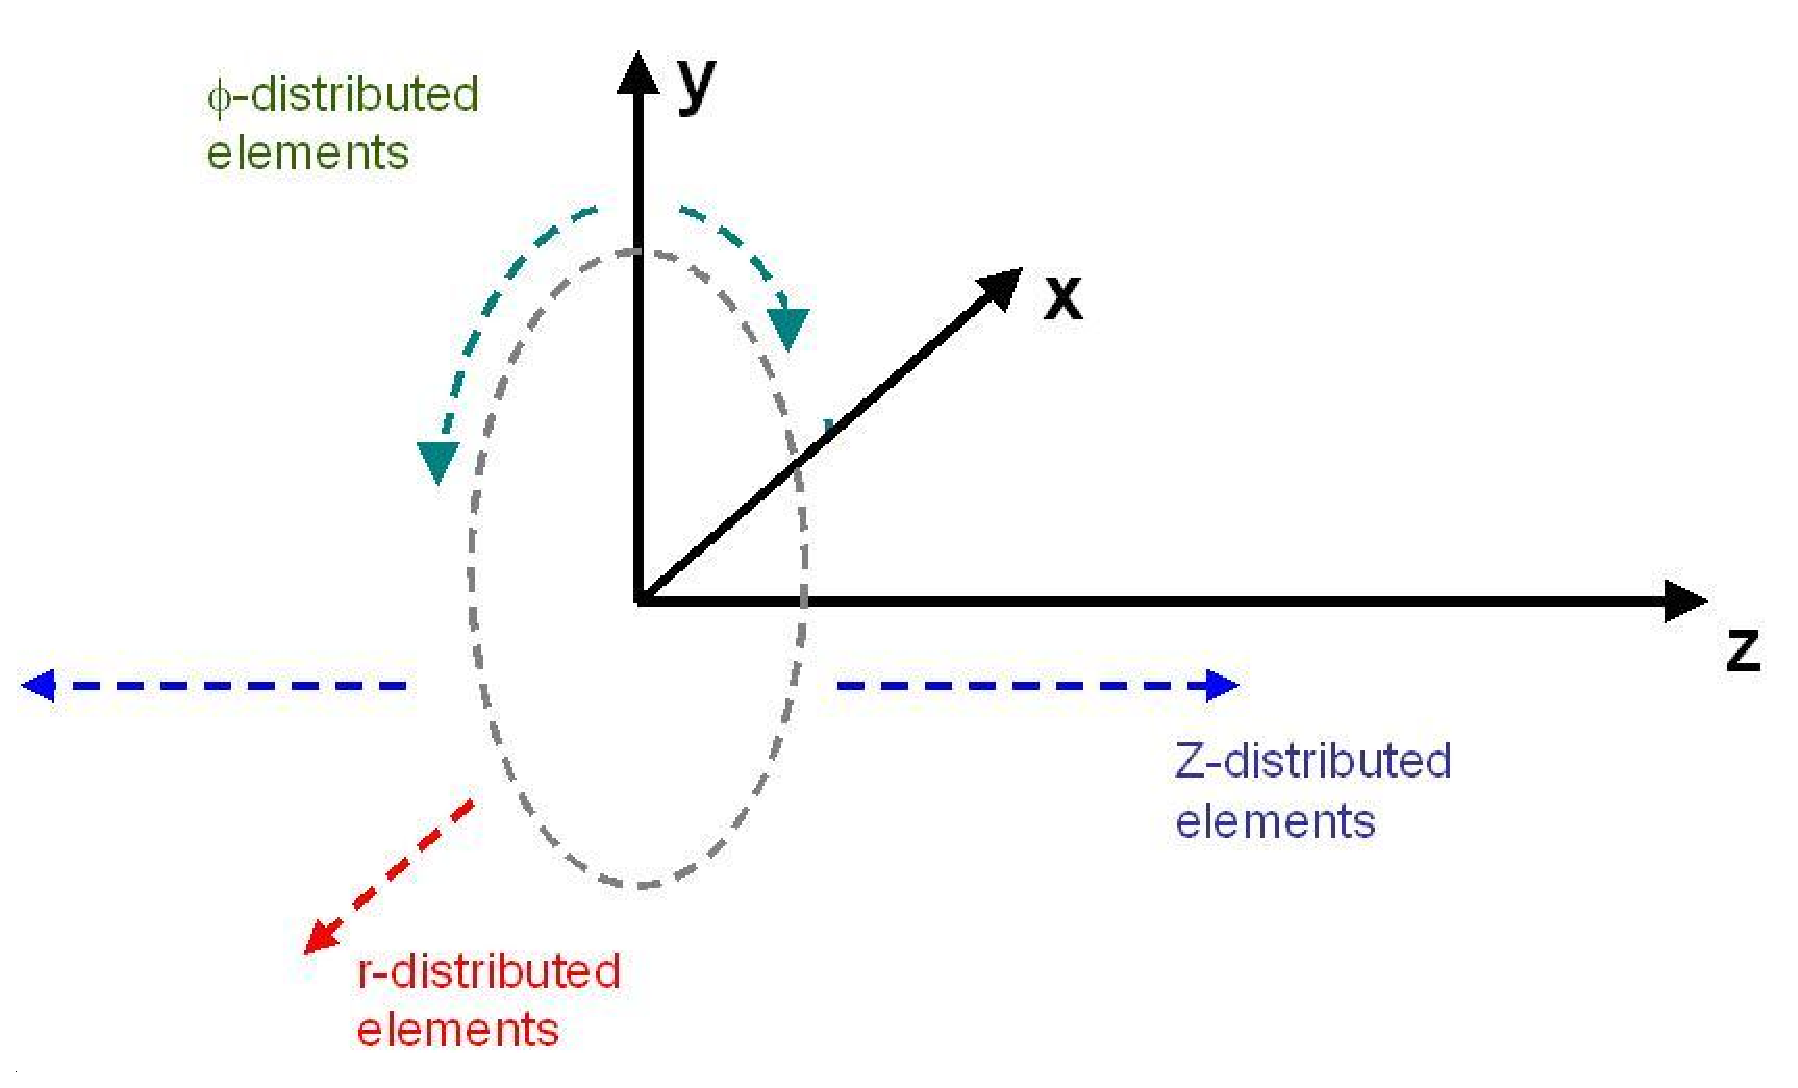
\epsfig{file = convention_v1.eps, height = 64mm}
%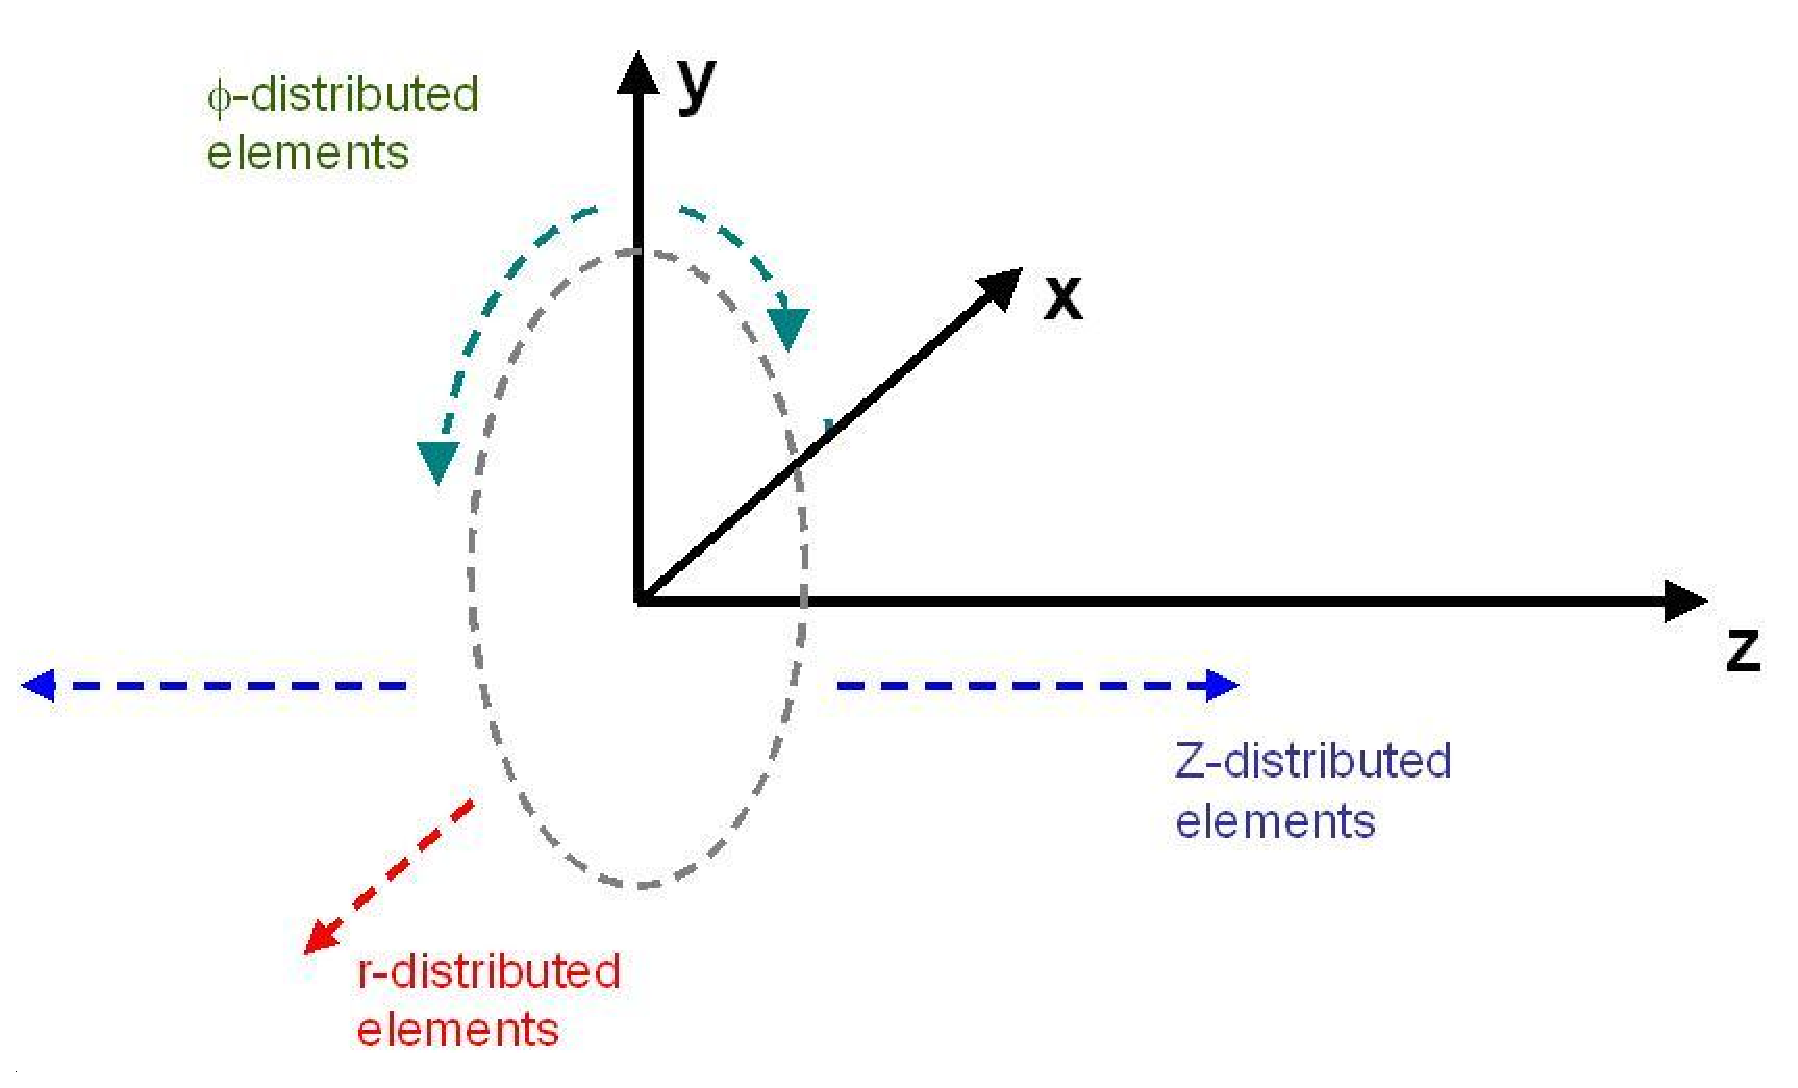
\includegraphics[width =0.8\textwidth]{convention_v1.eps}
    \caption{The general convention followed to label on-detector components.}
    \label{figure:convention}
  \end{center}
\end{figure}

Some of the names we propose will be closely connected to the geometric
layout of
the Pixel detectors and to their relation to the LHC interaction region. 
We have tried where possible to conform to
CMS conventions. Here we describe the ones relevant to this discussion. 

The global coordinate system of the CMS detector is defined to be a 
right-handed system, where the origin is 
at the Interaction Point (Interaction Point 5), 
the z-axis points in the direction of 
the magnetic field of the CMS solenoid, and the x-axis points towards
the center of the LHC ring. 
To the extent possible, we follow this convention in  identifying the 
components on the CMS Pixel detector.

For components that
are ordered along the $z$-axis, 
we group them into positive and negative z-axis first;
then name the component starting from one and increase the 
index with increasing distance from origin (IP). For $r$-distributed 
components, the index starts from one for smallest $r$ 
and increases with increasing $r$ value~\cite{DataModel}. 

For components that are segmented according to azimuthal angle, or $\phi$,
around the beam axis, we followed conventions that already existed within the
Barrel Pixel project.
It might seem natural and correct to start the azimuthal numbering from 
the x-axis.
However, because the pixel detector is split into two halves 
about the  y-z plane,
a more convenient way of labeling the $\phi$ components is to 
start from positive y-axis, increasing the azimuthal number index
with increasing $\phi$. 
For each side (+x and -x), $\phi$ segments are numbered beginning
with 1  at the top of the detector and increasing in number towards the
bottom of the detector. The largest number, N,  is adjacent to the negative 
y axis.  This means that the numbers 1 through N are repeated on both sides 
(+x and -x) of the y-z plane. 

To describe devices on opposite sides of the y-z plane, in other words
to describe whether the device is on the +x or -x side, we use the
names ``I'' (Inward) or ``O'' (Outward). Here Inward refers to devices
that are in the inside of the LHC beams or at +x; Outward refers to devices
that are outside of the LHC beams.

These conventions are illustrated in figure~\ref{figure:convention}. 


\section{Naming Convention for On-Detector Components}

The  components of the Pixel Detector are located in the CMS Collision Hall 
and in the Control Room. They can be divided into On-Detector Components
and Control Room Electronics. In this section, we present the naming convention
for on-detector components of the Forward and Barrel Pixel systems. Our 
approach is to first describe the system well enough to follow the main 
hierarchical organization and naming convention down to the individual 
silicon pixels. Then, we 
complete the discussion by retracing the hierarchy focusing on
the naming convention for electronics 
boards and the programmable chips and monitoring elements
associated with them.  

The naming convention is based on the physical organization of the
pixel detector. It can be viewed as a hierarchical organization starting
from pieces that are a quarter of the full Forward respectively Barrel Pixel detector and winding up at an
individual pixel. The naming convention lists the levels of
this hierarchy with each level separated by an underscore (\_). 
In most cases, there are more than one instance of the hierarchy and
these are differentiated by either letters such as `a' or 'b' or numbers
usually comprising a range. In the naming convention, we denote
choices between a few options by listing the option letters, numbers,
or names in parentheses: (option1, option2). If there are a range of numbers,
instead of listing them all, we write it as (N... NL).
If the range can have a variable length, it is written as
(NF... (NL1,NL2)). 
In some cases, it is necessary to provide names for attributes of a level of 
the hierarchy. These attributes are typically writable or readable registers
of a physical device.These are separated from the name of the hierarchy level 
to which the attribute applies by a hyphen (-). 

An example of  the hierarchical name down
to a single pixel illustrates all of these conventions:
\begin{displaymath}
\mbox{FPix\_B(p,m)(I,O)\_D(1-3)\_BLD(1-12)\_PNL(1,2)\_PLQ(1-(3,4))\_
ROC(0-(1,4,5,7,9))-DACNAME}
\end{displaymath}
The explanation of this entire string will be given item-by-item below.


\subsection{The Forward Pixel System}

\subsubsection{The Forward Pixel Hierarchy}

The names of the Forward Pixel on-detector components always start with 
FPix to distinguish  them from the Barrel pixel detector. The components on
the positive z-axis side  and the negative z-axis side 
with respect to the IP are prefixed with Bp 
and Bm, respectively. 
On each side of the IP, the detector is composed of two half-cylinders
that concentrically surround the beam line, 
the Inward (I) and Outward (O) half-cylinders.
%Here, Inward refers to devices that point to the center of the LHC ring 
%(i.e. are at the +x side of the y-z plane),
%while Outward refers to devices that point outside of the LHC ring
%(i.e. are at the -x side of the y-z plane).
Thus, there are four major components in the FPix detector,
named FPix\_BpI, FPix\_BpO, FPix\_BmI, and FPix\_BmO. 

One of the four half-cylinders of the Forward Pixel detector is shown in fig.~\ref{figure:FPix}.
In order to make its components more visible, the figure shows the half-cylinder rotated 
from its normal vertical orientation.

\begin{figure}[hbtp] 
 \begin{center} 
%        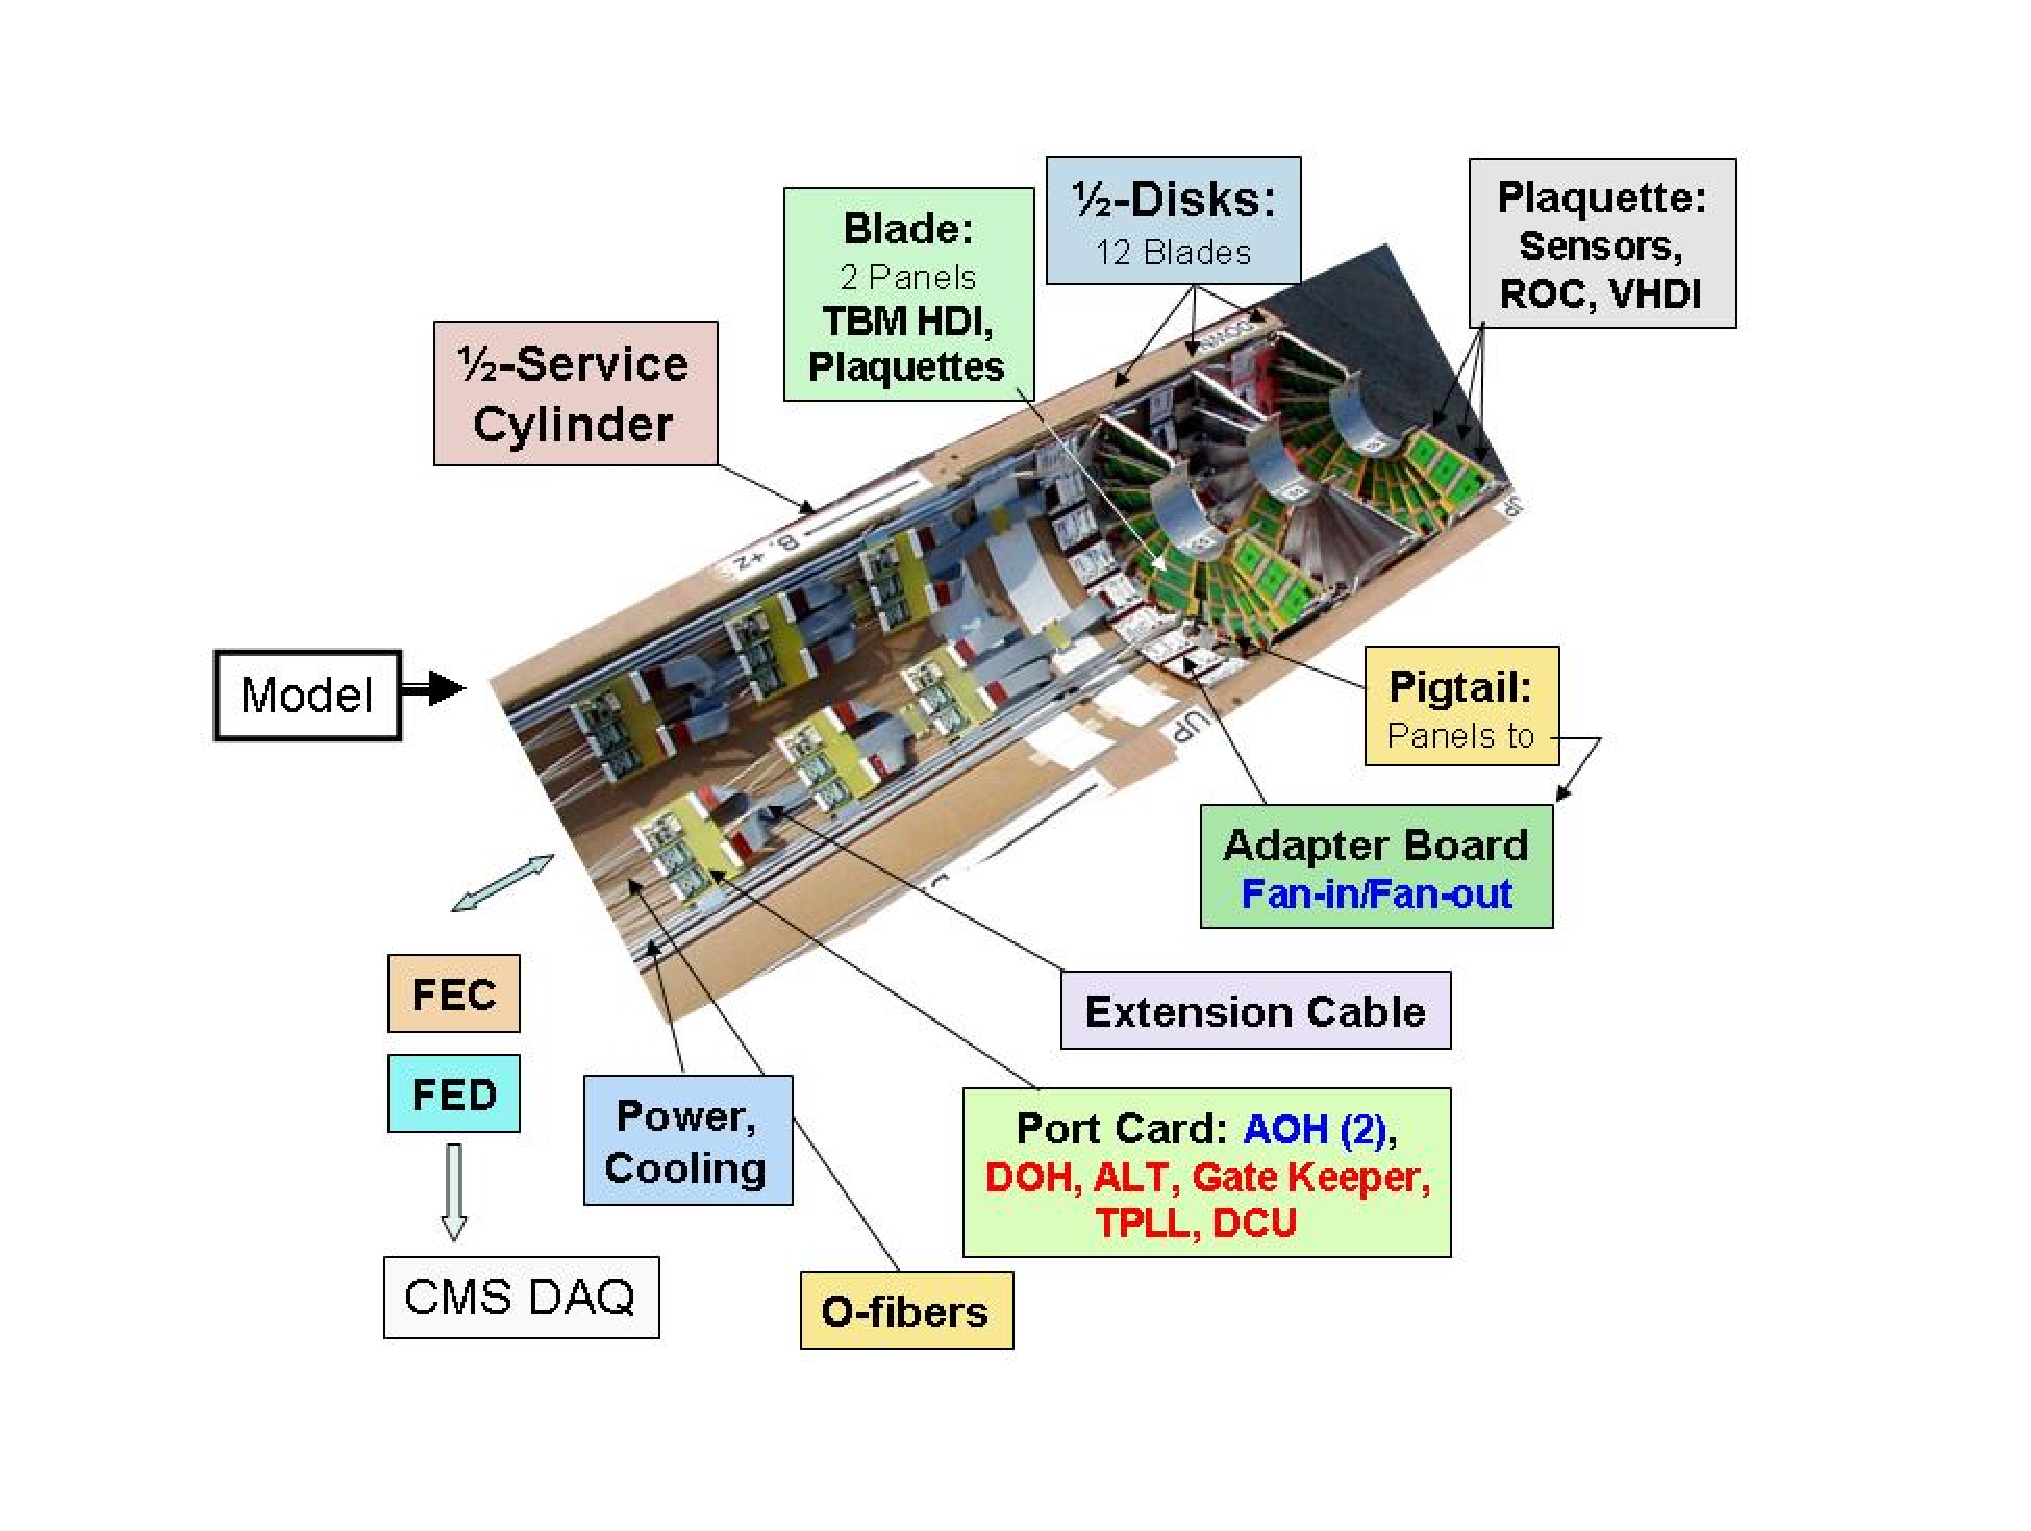
\includegraphics[width =0.6\textwidth]{fpix_overview.eps} 
        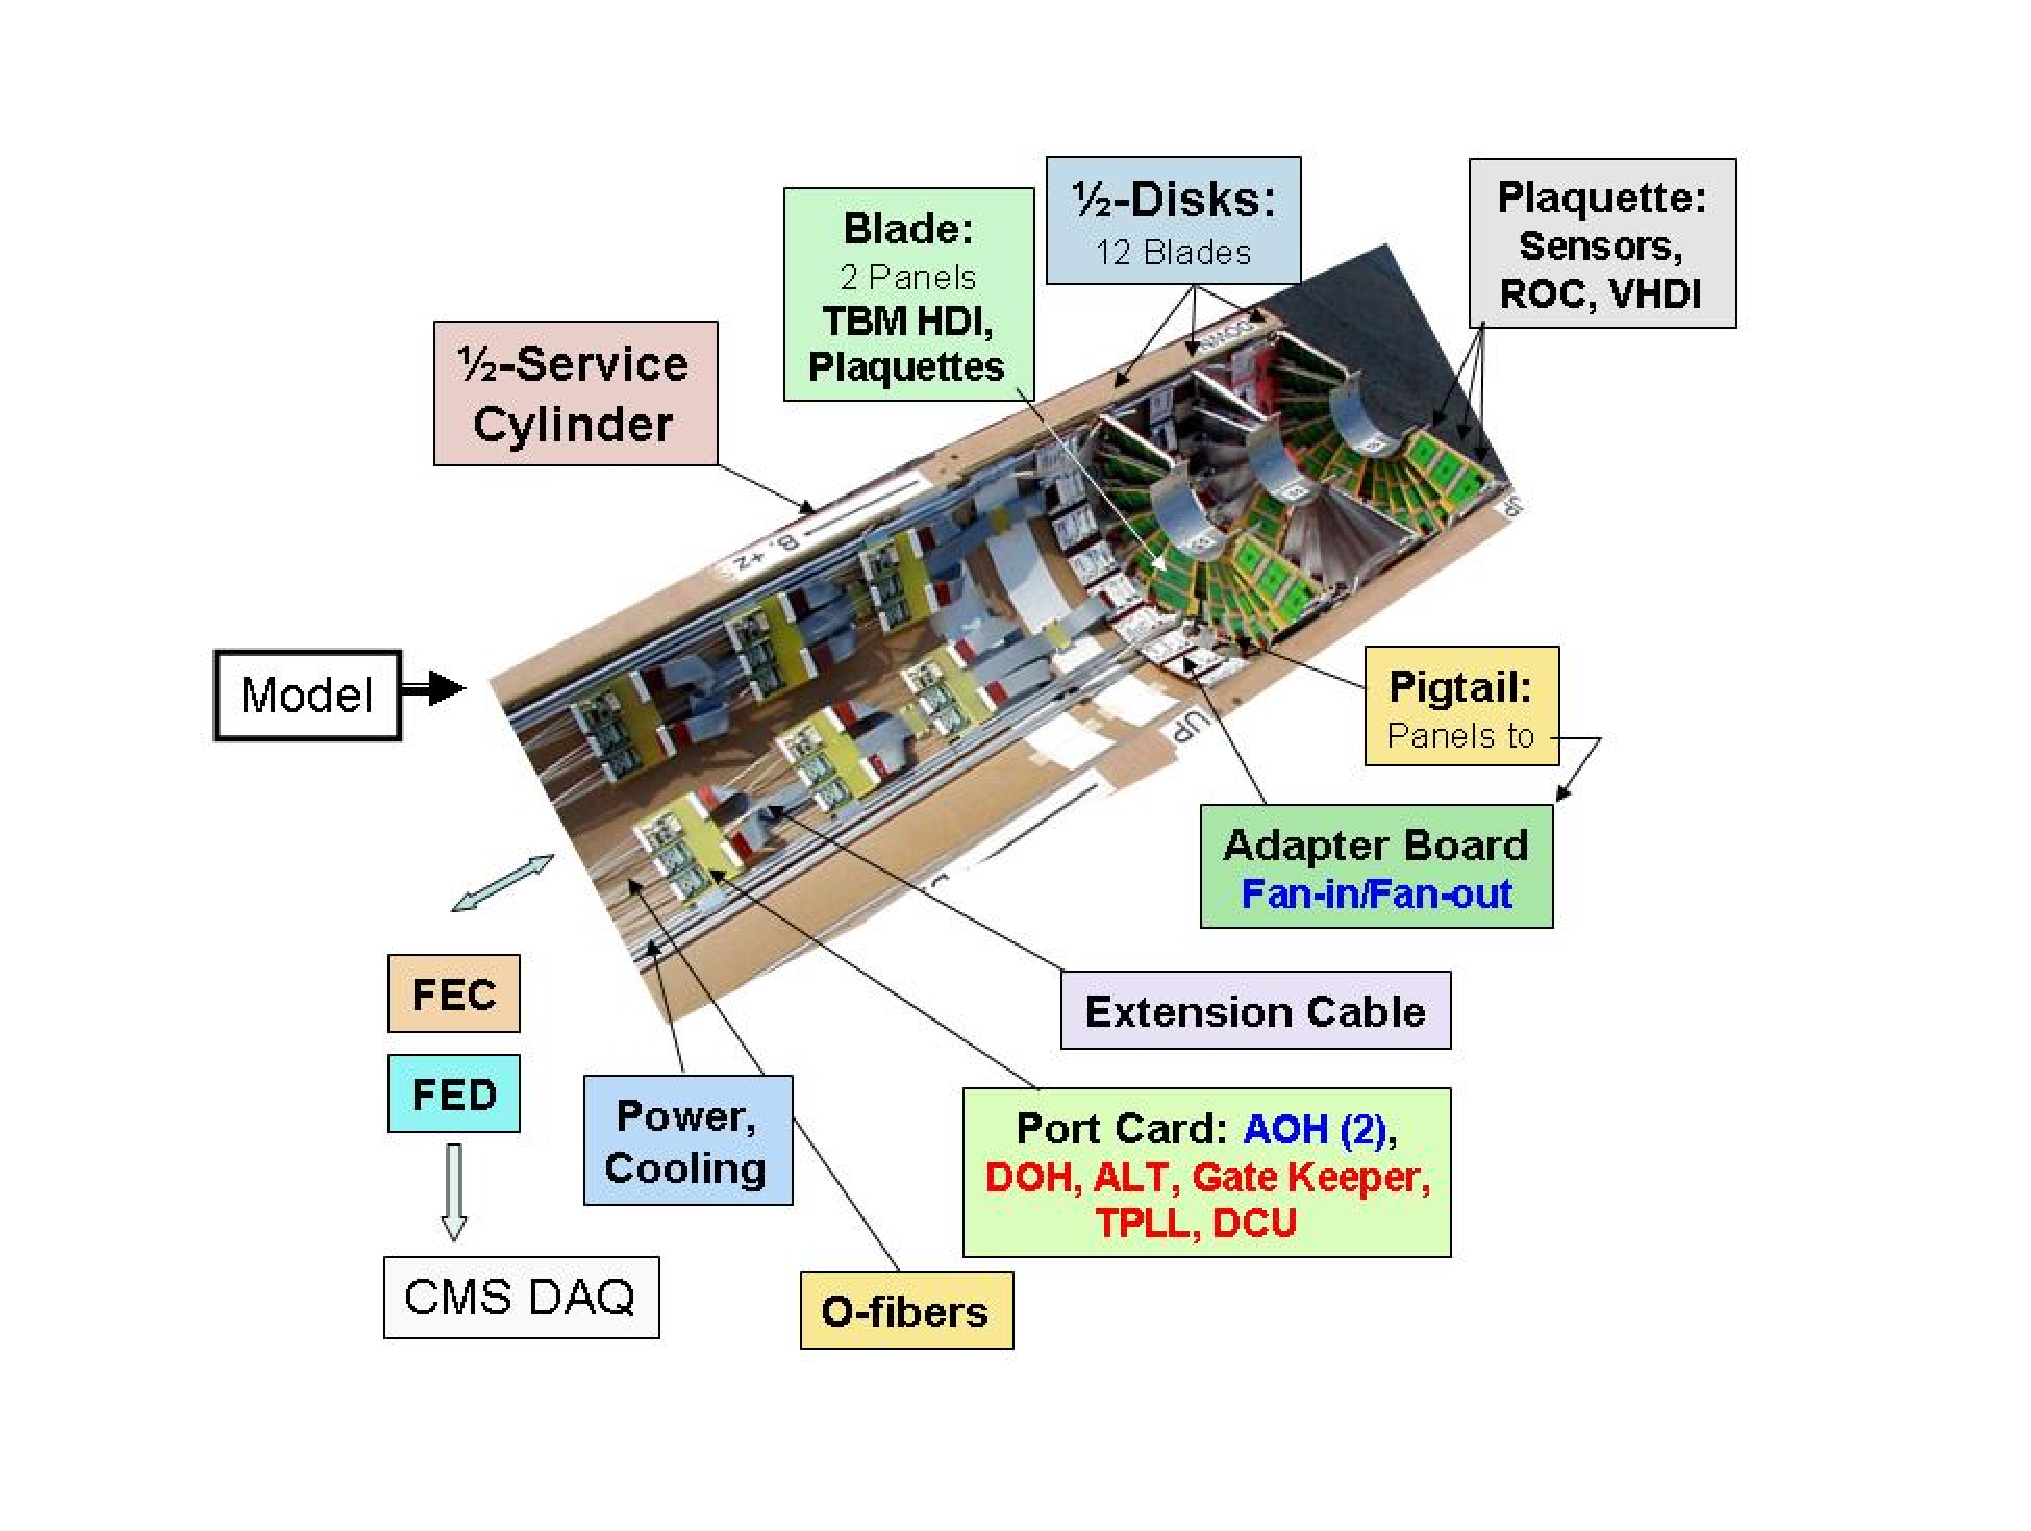
\epsfig{file = fpix_overview.eps, height = 70mm,
                bbllx=91, bblly=76, bburx=829, bbury=656, clip=}
    \caption{Block of components for the BpO half-cylinder of the 
  Forward Pixel detector.    \label{figure:FPix} }
   \end{center} 
\end{figure} 


Each half-cylinder consists of two active detector elements called half-disks.
The half-disks  have an inner radius of 6 cm and an outer radius of 15 cm
and are located at two different z positions along the service cylinder.
The first is located at 34.5 cm from the IP and the second 46.5 cm from the IP
\footnote{Provision is left for a third half-disk at 58.5 cm in a future upgrade.}. 
The half-disks are named D1 and D2 (and D3), with D1 being the closest to the IP. 

Each half-disk is divided into azimuthal sectors called ``blades'' that subtend
an angle of 15$^{\circ}$. There are 12 of these per half-disk. As described 
above, the blade that  begins at the top of the detector is labeled
BLD1 and the blade at the bottom is labeled BLD12. 

Fig.~\ref{figure:azimuthal_numbering} is a schematic representation of the 
blades for the two disks closest to the IP showing the numbering.

\begin{figure}[hbtp]
  \begin{center}
    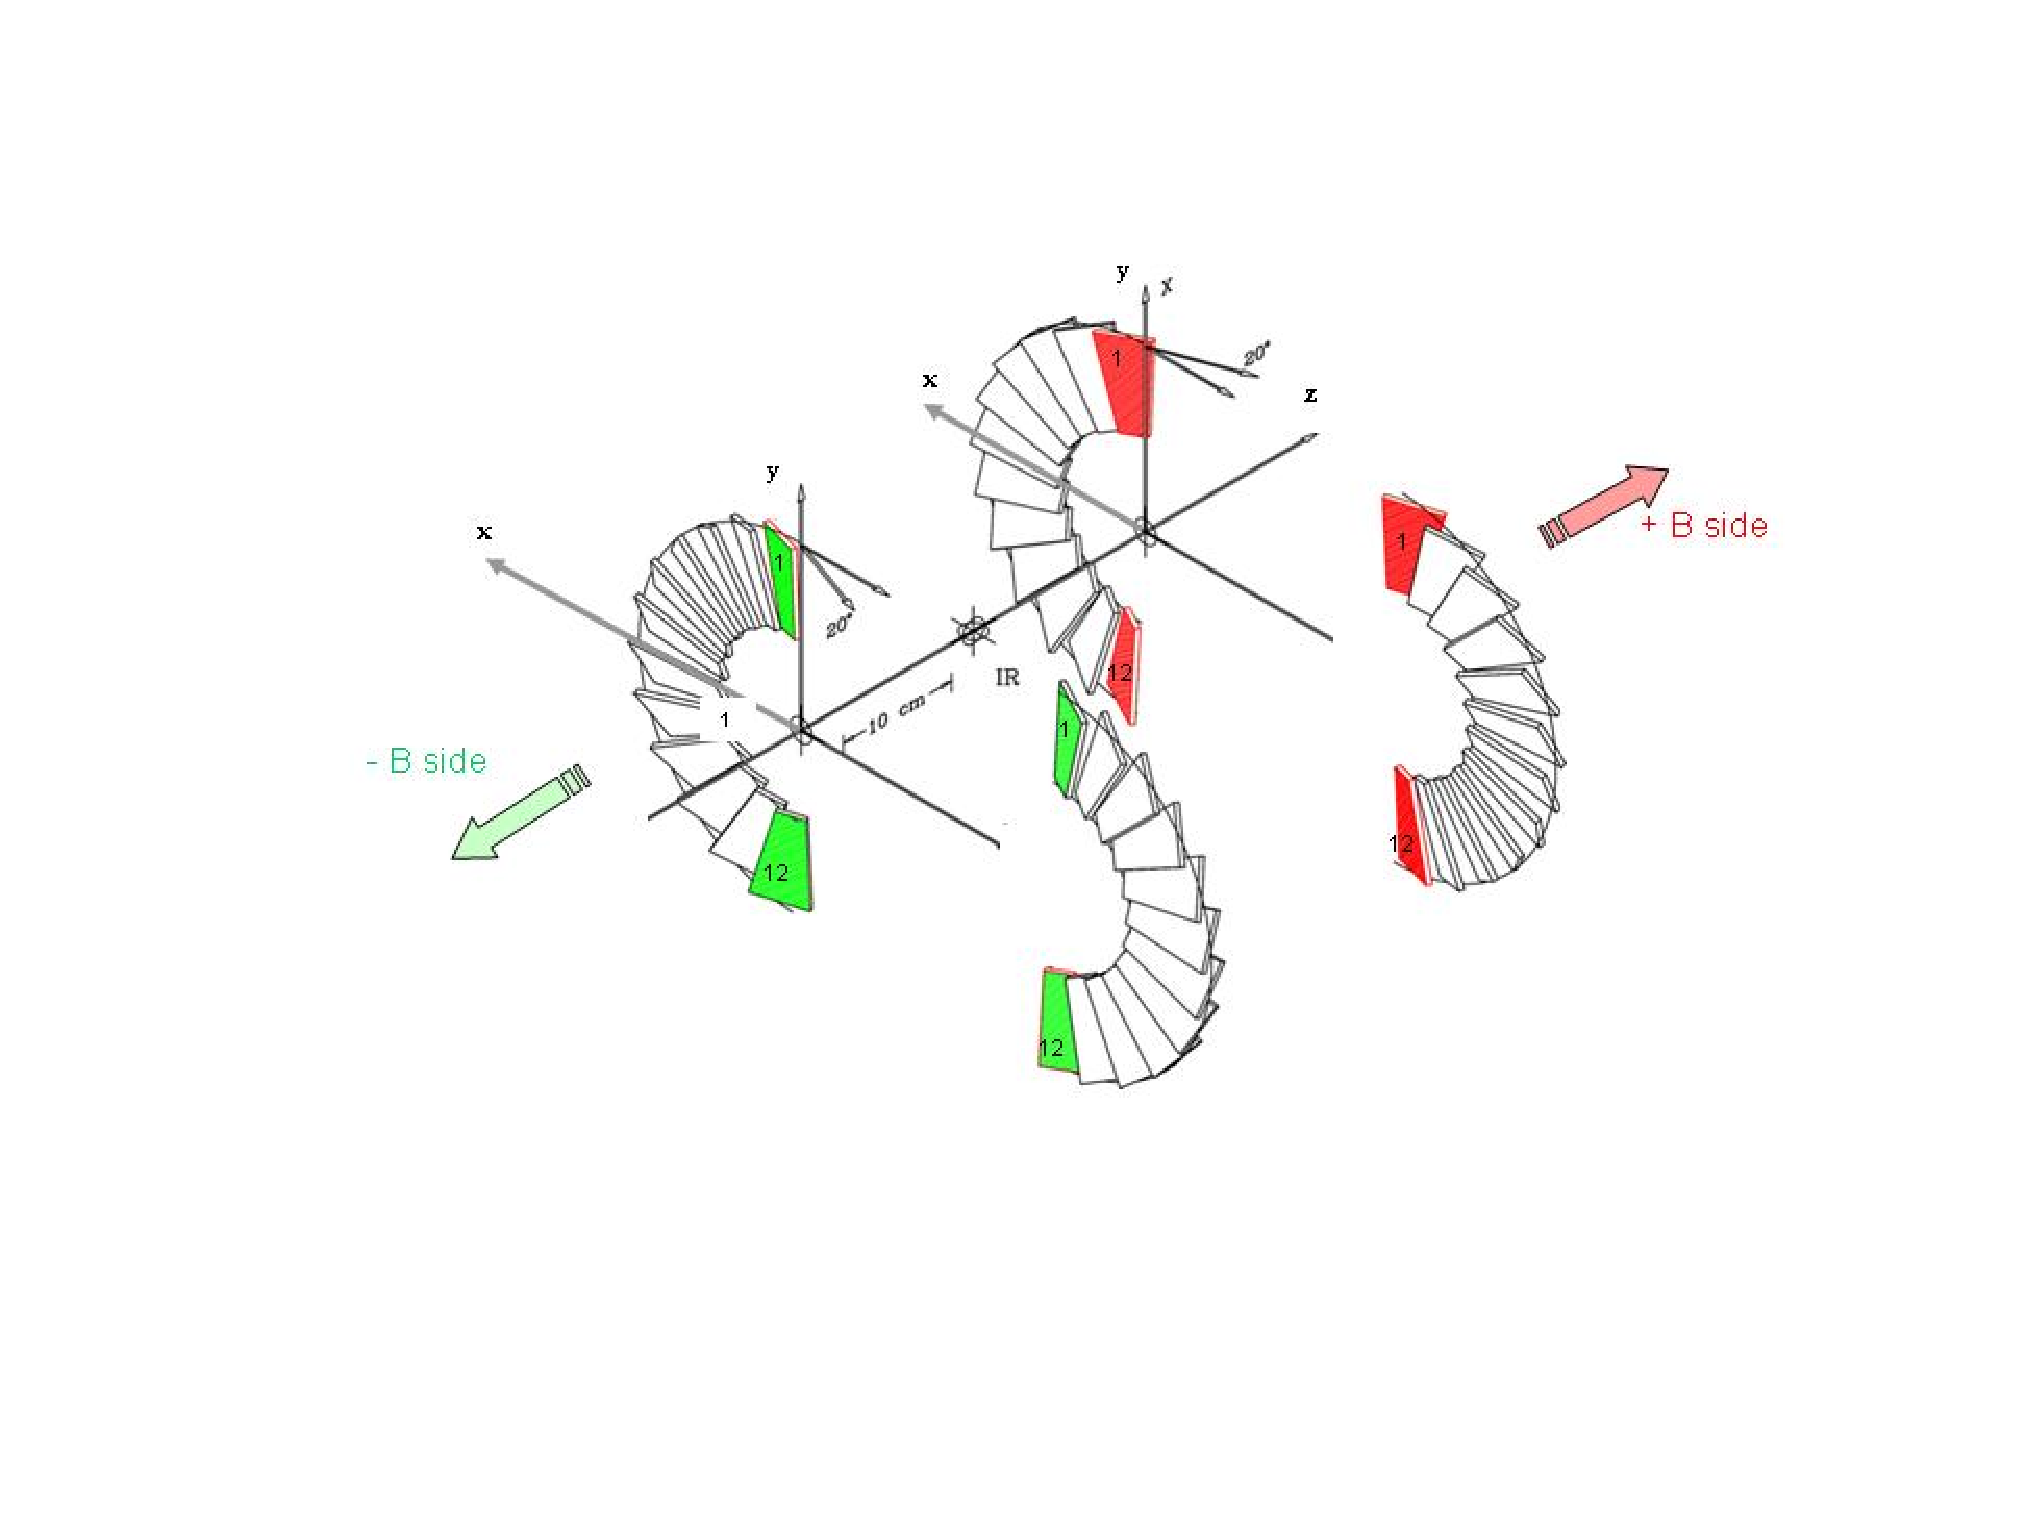
\epsfig{file = Azimuthal_numbering.eps, height = 80mm,
            bbllx=161, bblly=198, bburx=843, bbury=602, clip=}
 %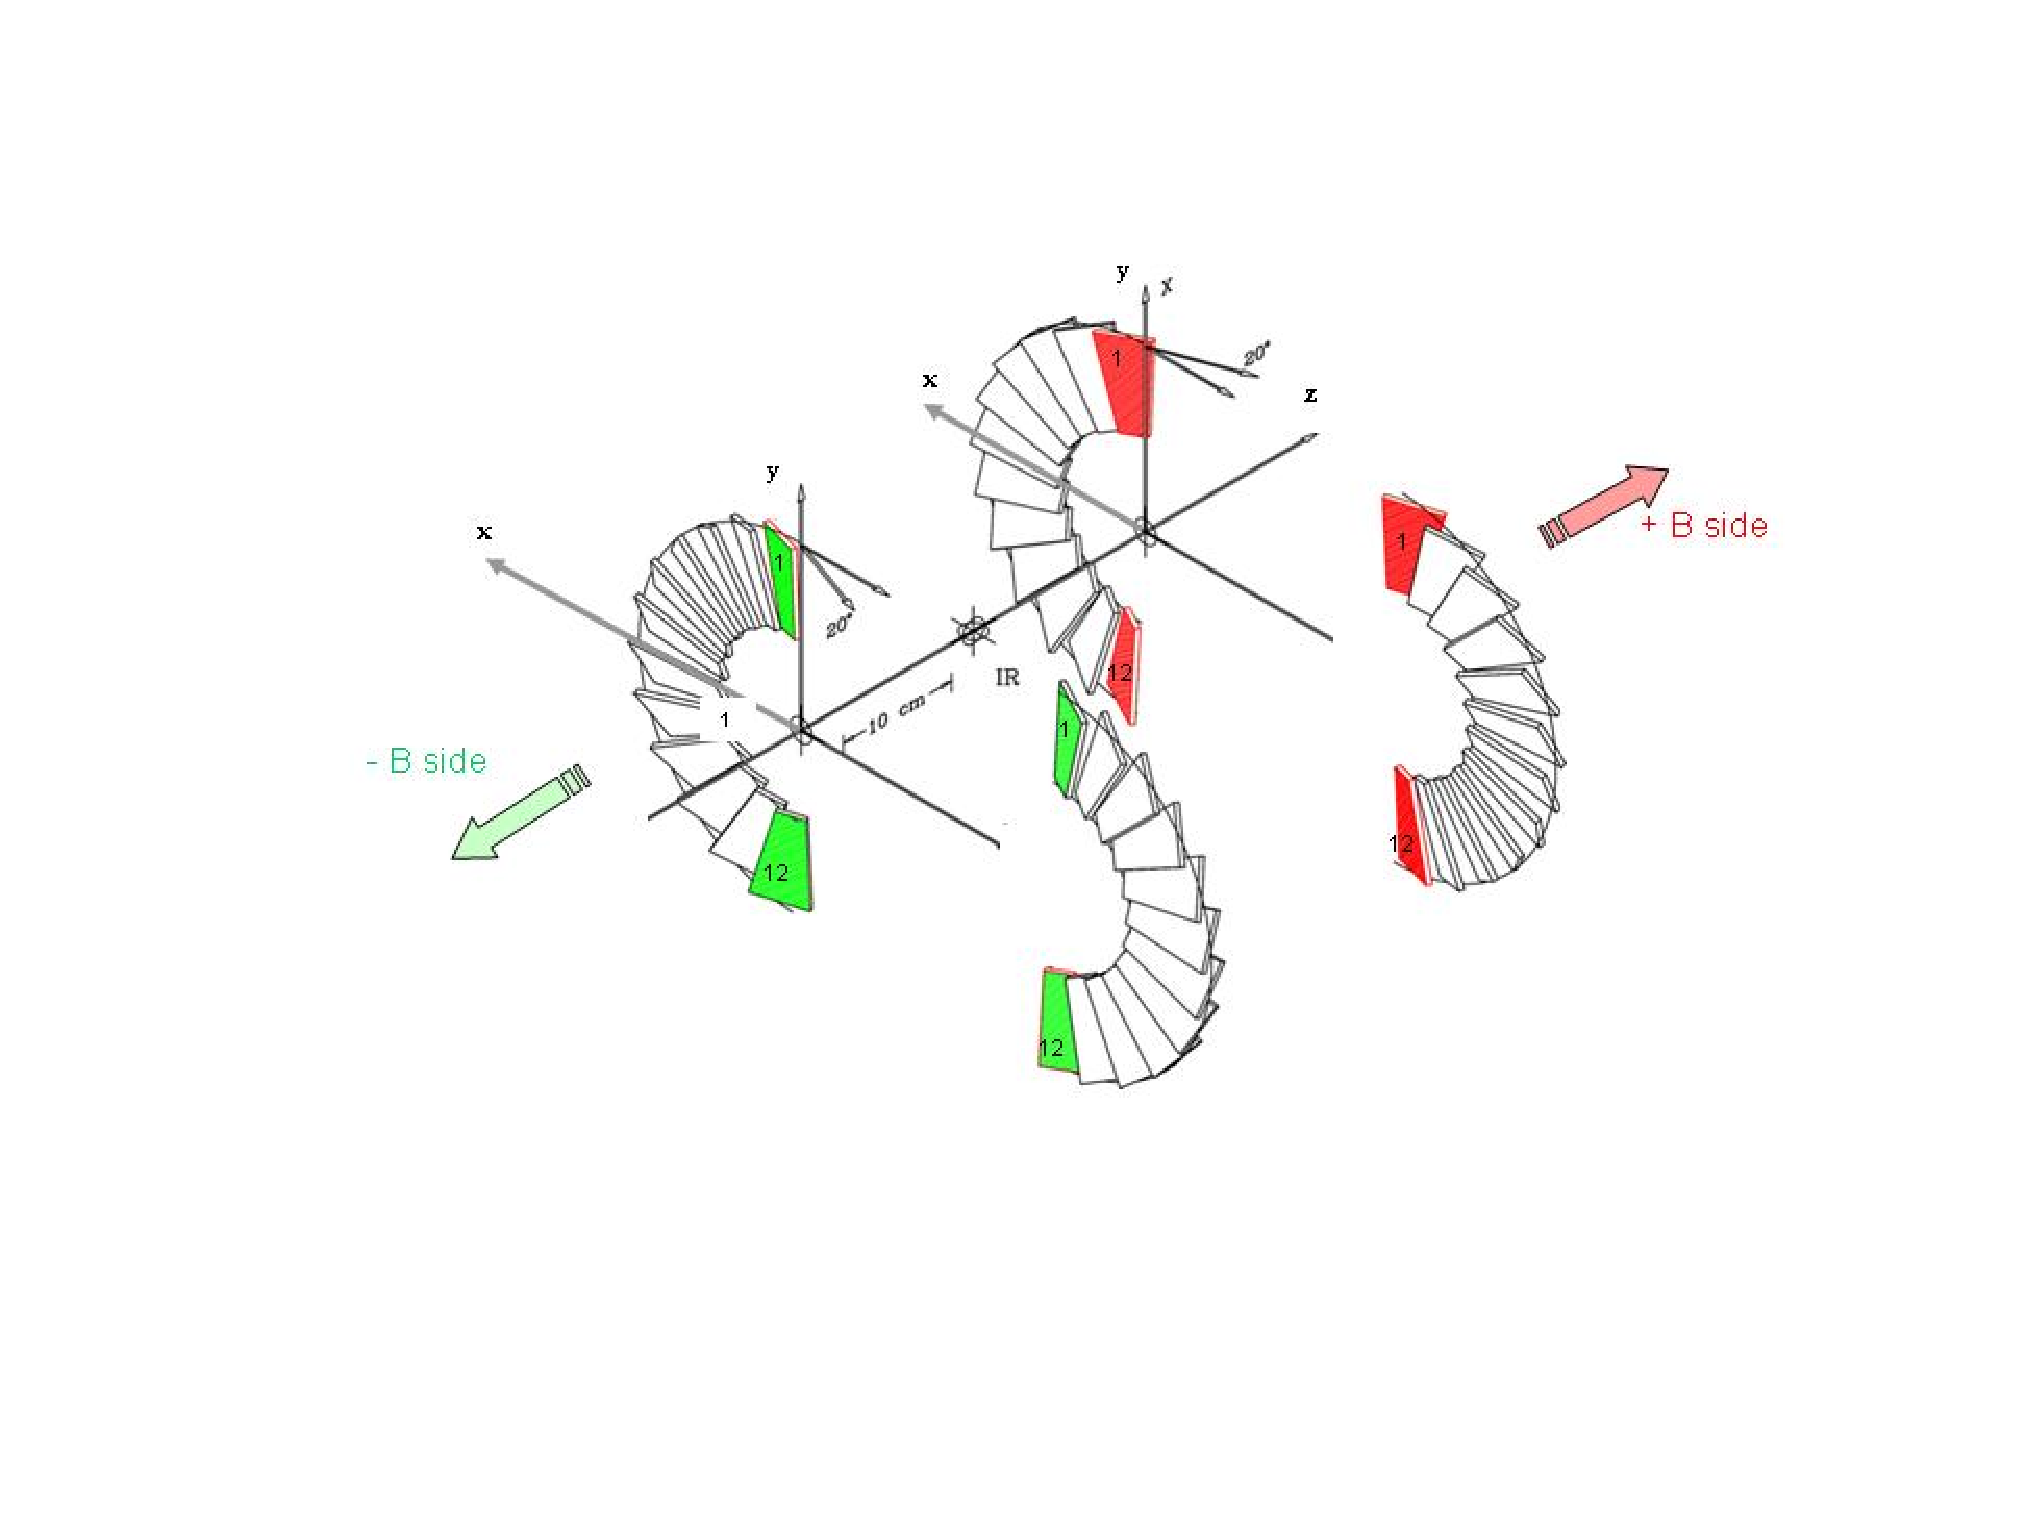
\includegraphics[width =0.8\textwidth]{Azimuthal_numbering.eps}
    \caption{Numbering convention for blades on half-disks}
    \label{figure:azimuthal_numbering}
  \end{center}
\end{figure}

The blades consist of a cooling structure with two 
trapezoidal ``panels'' mounted on either side of the structure, 
one on the so-called upstream side nearer the IP and the other on the downstream side farther from the IP. 
The two panels are labeled PNL1 and PNL2, respectively. 

Up to this level, a blade is named as
%\begin{displaymath}
$\mbox{FPix\_B(p,m)(I,O)\_D(1-3)\_BLD(1-12)}$
%\end{displaymath}
and a panel  on it can be referred to
as
%\begin{displaymath}
$\mbox{FPix\_B(p,m)(I,O)\_D(1-3)\_BLD(1-12)\_PNL(1,2).}$
%\end{displaymath}

The two panels are instrumented with ``plaquettes'',
which are the active detector elements of the FPix detector and consist of
a silicon pixel sensor electrically connected to an array of readout chips, 
referred to as ``ROCs'', by a process called bump-bonding.
There are four plaquettes on an upstream panel, PNL1.
The plaquettes are numbered from 1-4 with numbers increasing with radial distance from the beam line. 
On the downstream  panel, PNL2, there are three plaquettes,
which are numbered from 1-3, again with numbers increasing with radial distance from the beam line.

The plaquettes are produced in different sizes.
The different sizes are needed to cover the trapezoidal 
shape of the panels. 
Accordingly, the silicon pixel sensors are produced in five different sizes too
and are bump-bonded to arrays of different numbers of readout chips.
Plaquette types are referred to by the numbers of rows (1 or 2) times the number of columns,
in the array of readout chips bump-bonded to the silicon pixel sensor.
The actual types required to cover the  panels are 
1x2, 1x5, 2x3, 2x4, and 2x5. The four types of plaquettes on PNL1 are  1x2,
2x3, 2x4, and 1x5. The three types on PNL2 are 2x3, 2x4, and 2x5.
The numbering of the plaquettes on the panels is shown in 
Fig.~\ref{figure:roc_numbering}.


%%\begin{figure}[hbtp]
%%  \begin{center}
%%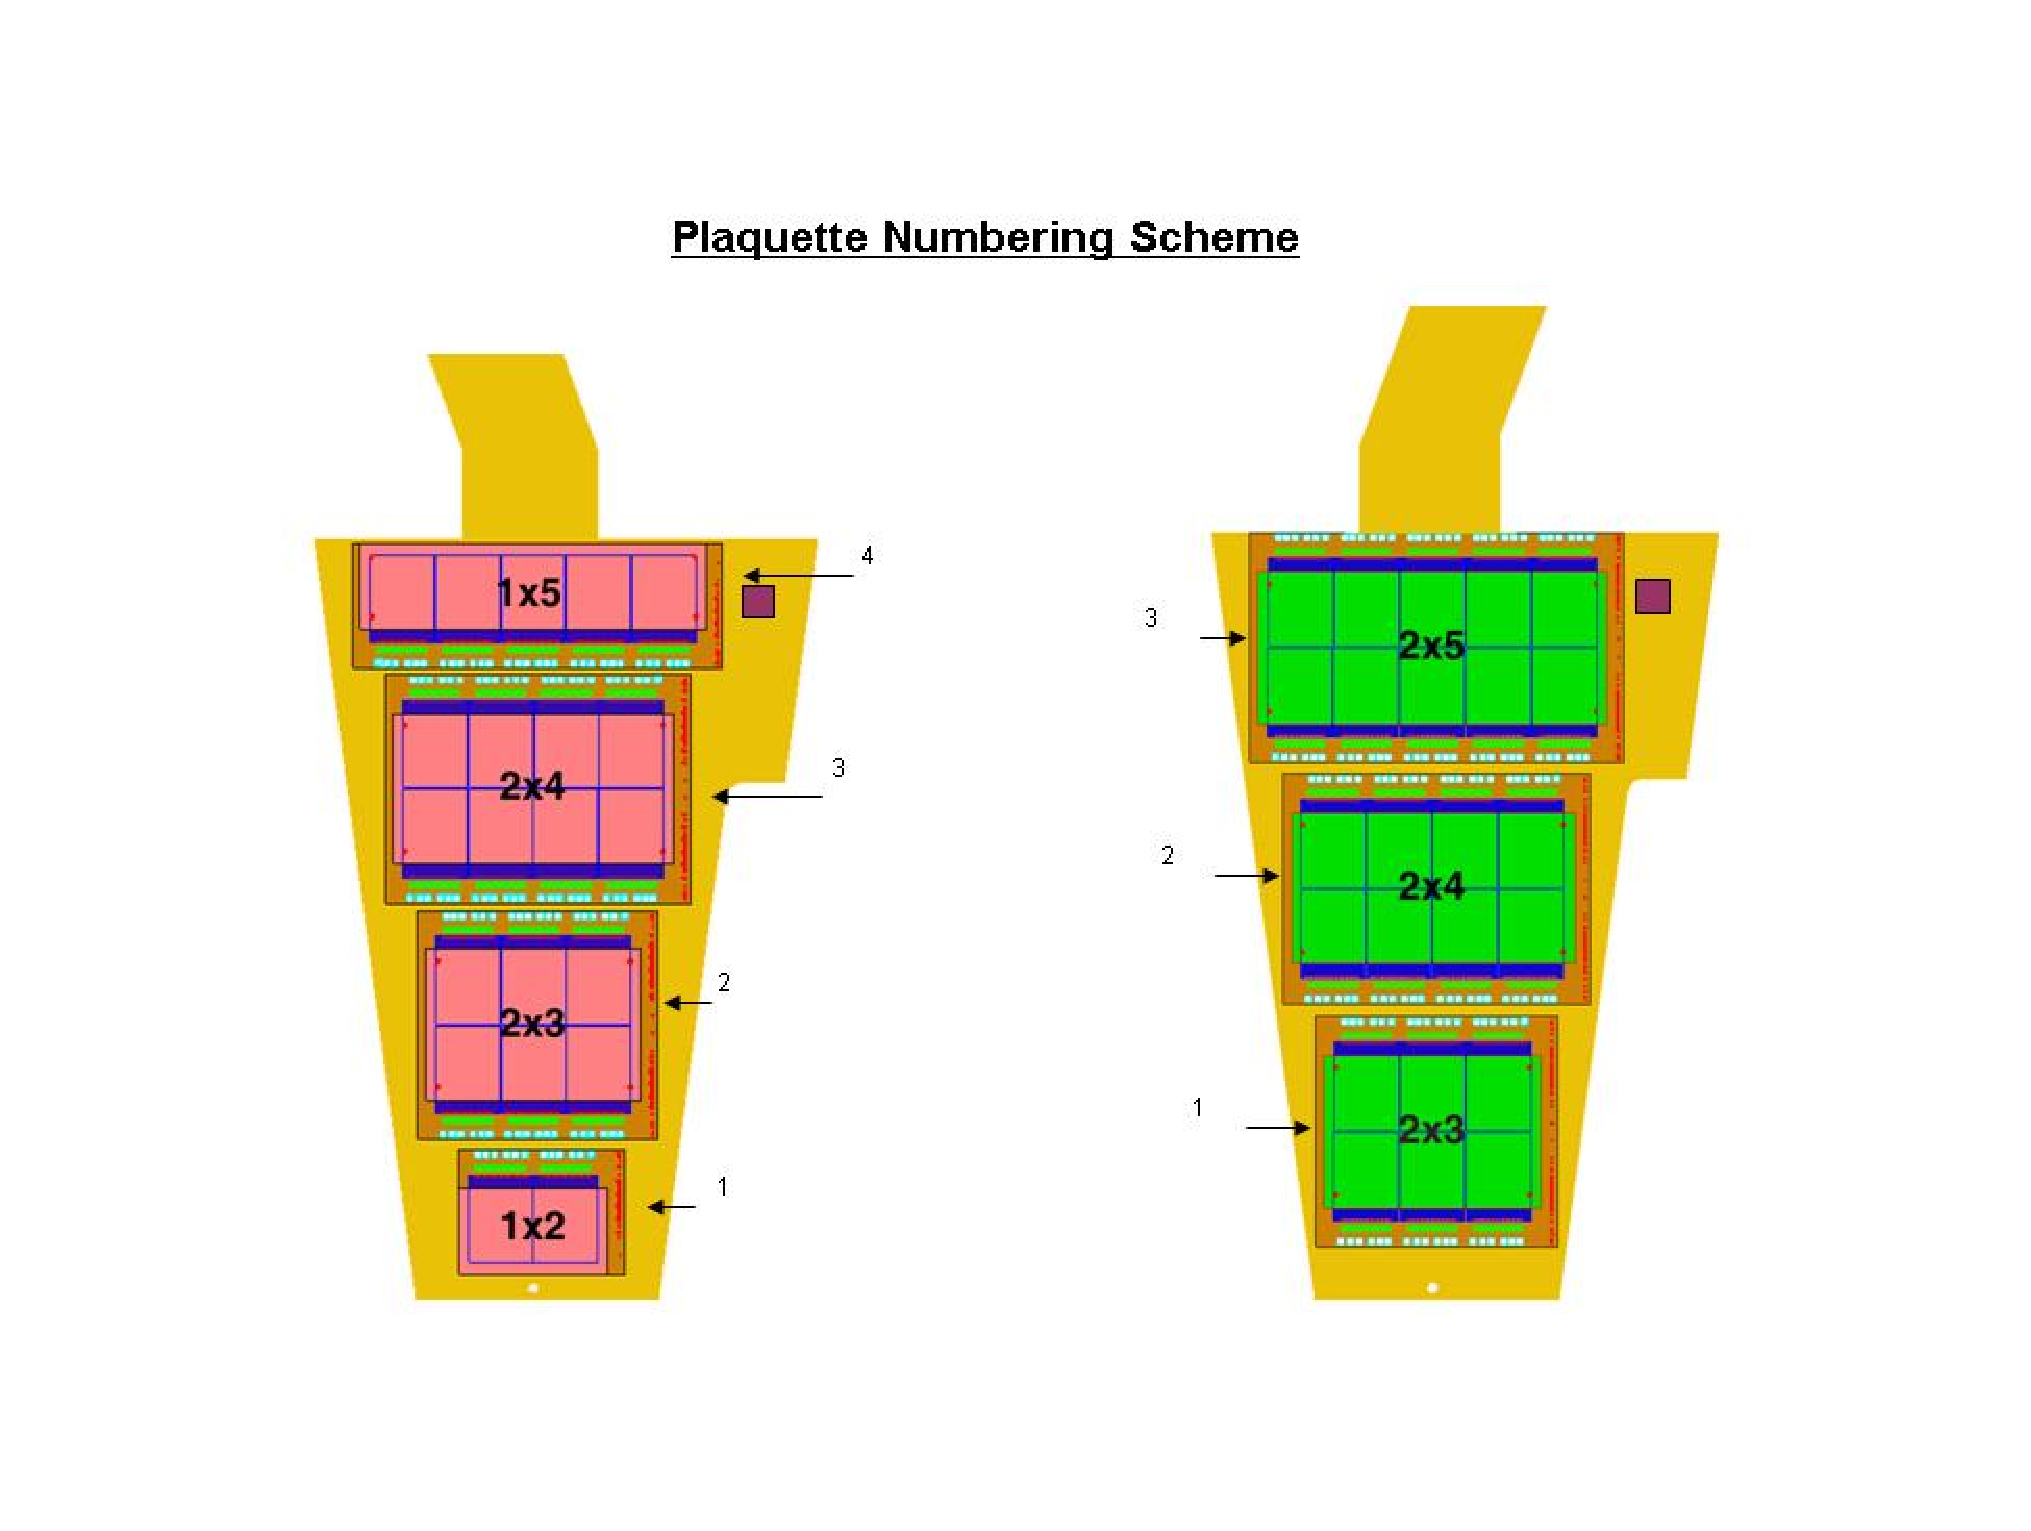
\includegraphics[width =0.8\textwidth]{Plaquette_Numbering.eps}
%%    \caption{Numbering convention for plaquettes on
%%            the two types of panels. }
%%    \label{figure:plaquette_numbering}
%%  \end{center}
%%\end{figure}

The  ROCs are numbered from 0 to n-1 
(n up to 1, 4, 5, 7, or 9; for 1x2, 1x5, 2x3, 2x4, and 2x5 plaquettes; respectively). 
This indexing is used to address the internal registers of the ROCs,
as is discussed below.


The ROCs on each panel are read out sequentially by a token-passing scheme 
managed by a chip, called a ``TBM'' (the ``Token Bit Manager''),
one of which  is mounted on each panel. The data from the ROCs
do not contain the ROC address on the plaquette but
rely for their interpretation on the
order in which the ROCs appears in the data stream output by the TBM 
(a header is output to the data stream by each ROC even in case no pixel have hits).
The order of the ROC numbering in the output data stream follows 
the order in which the token is passed and varies for different types of
panels (there are four types) based on electrial and mechanical considerations
that would only be obvious to the designers. For control and configuration 
purposes, the TBM addresses ROCs using the PSI$^2$C protocol via particular
port addresses, another complication discussed below.
For this reason, we adopt a 
numbering convention for ROCs that is based on geometic considerations
and is easier for a human being to remember. The convention is based on
looking at the active components on the panel (which are
toward the IR  for panel 1 on a 
blade and are away from the  IR for panel 2 on a blade). 
For each plaquette, the 
ROC on the lower left of the plaquette is numbered ZERO and the numbers 
increment from left to right on the first row and if there is a second row 
for the plaquette, the numbers continue to increment from right to left, or anticlockwise.
This  is shown  
in Fig.~\ref{figure:roc_numbering}. Since there are now several numbering
schemes for the ROC on a panel that need to be differentiated, we call this 
number the ``ROC Location Index'' or ``RLI.'' Tables are needed to 
translate this number to an corresponding PSI$^2$C address, to an order in
the ultrablack frame of the panel readout, and to the address as it appears in 
the online and offline software. The mapping tables are given in 
appendix~\ref{app:CrossReferencePixelIndices}. 

\begin{figure}[hbtp]
  \begin{center}
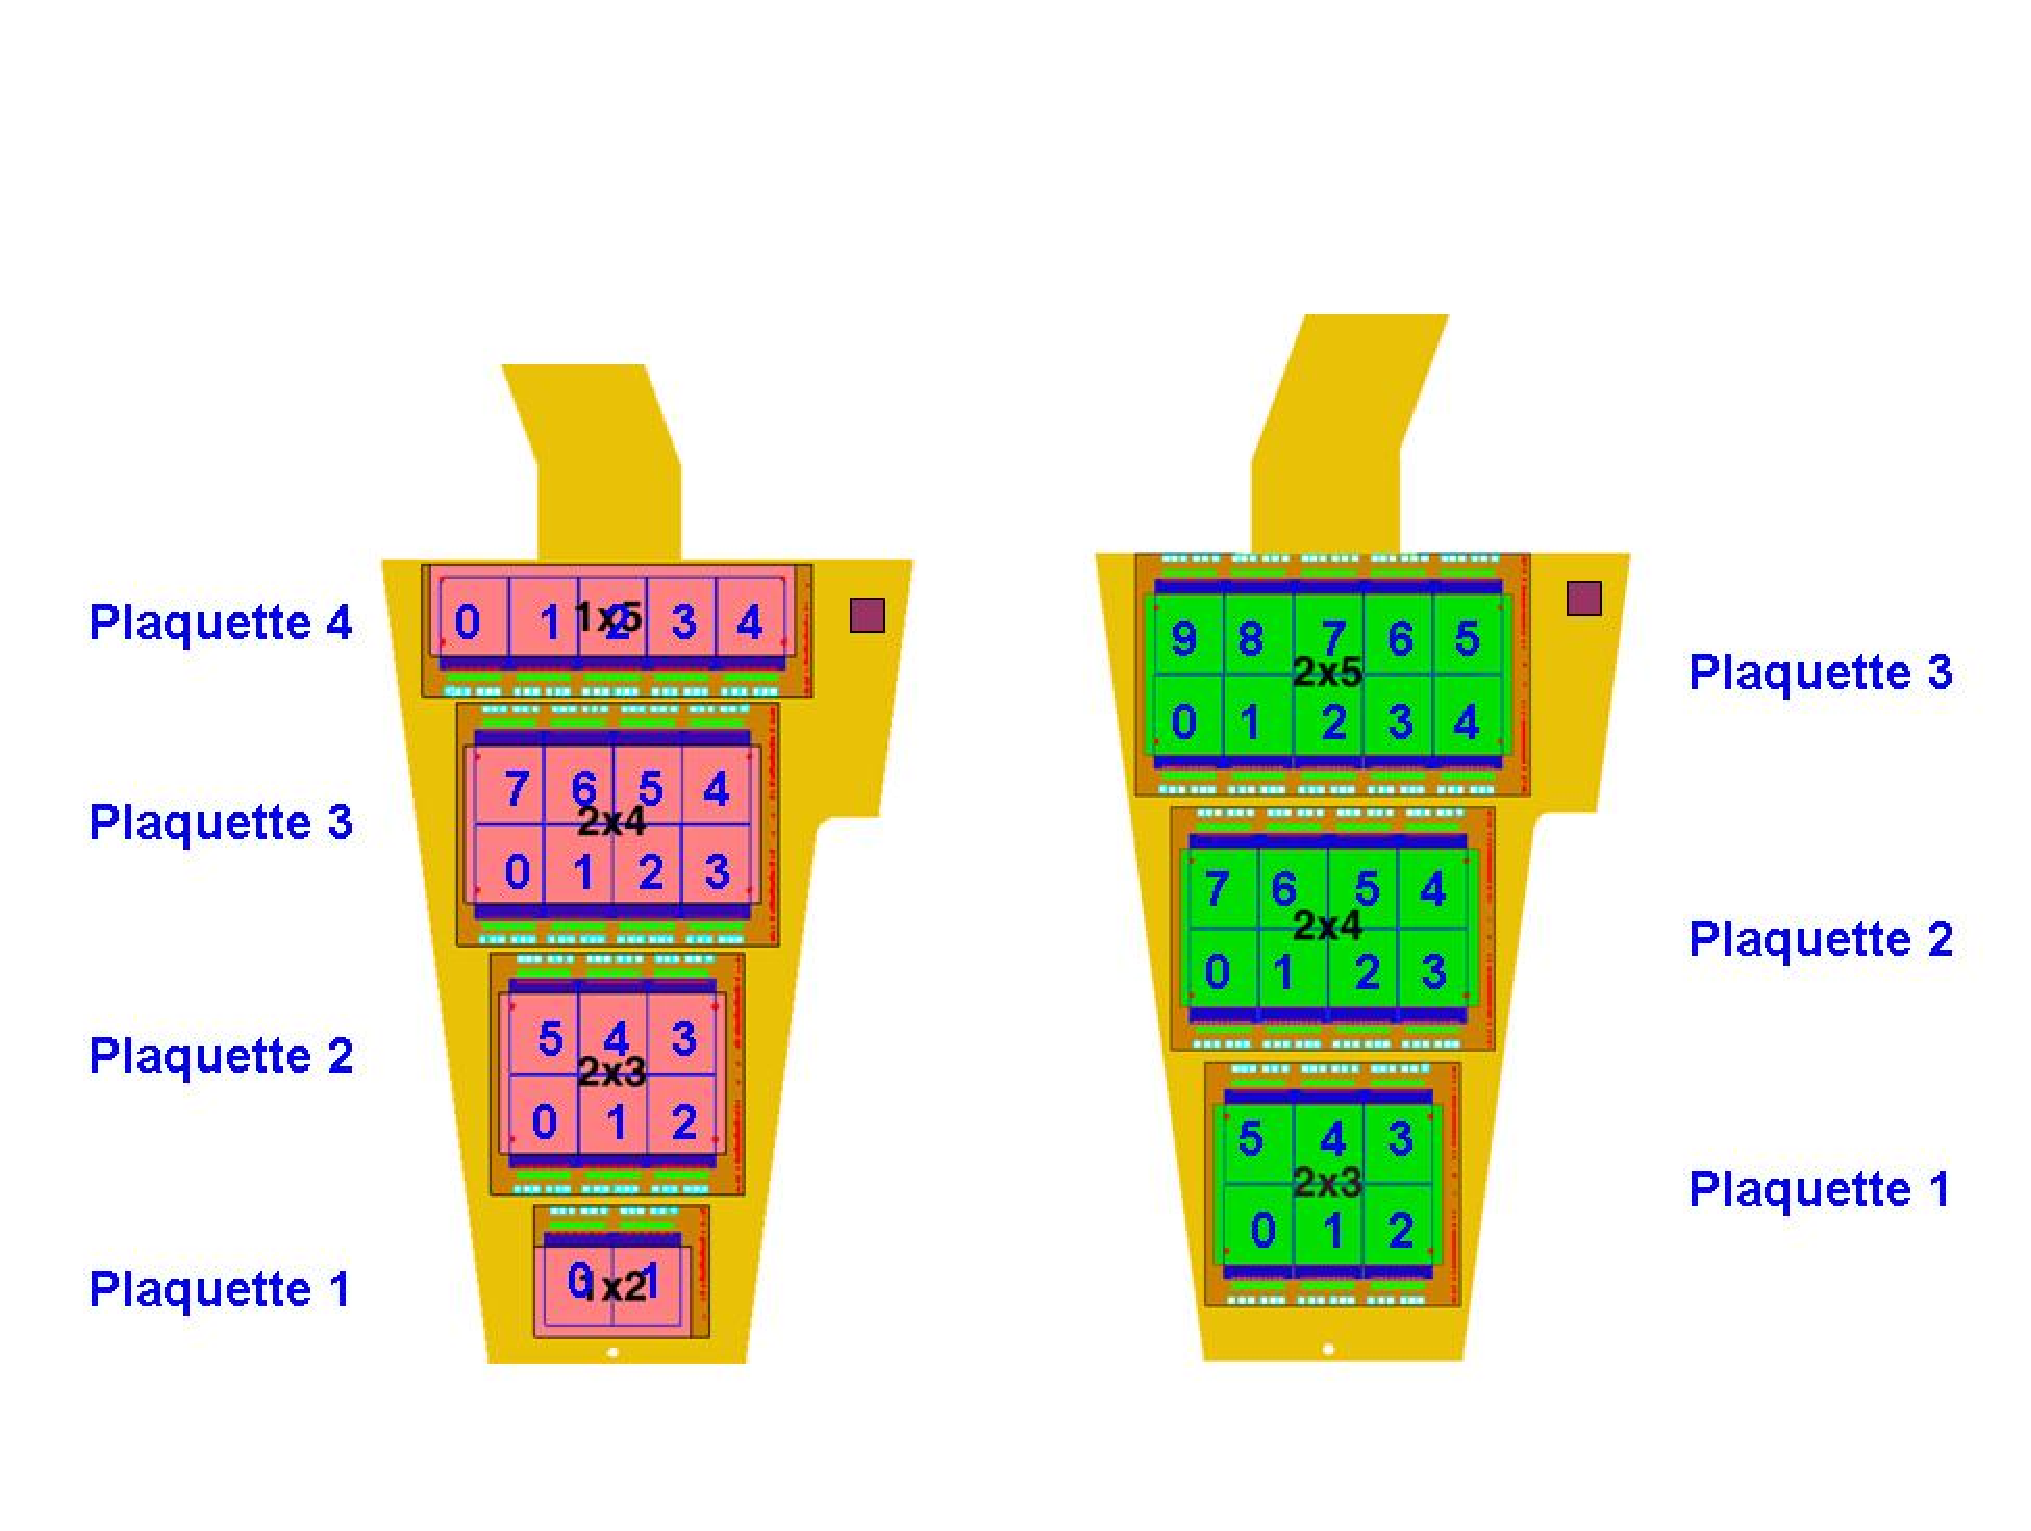
\includegraphics[width =0.8\textwidth]{ROC_config_numbers.eps}
    \caption{Numbering convention for Plaquettes and ROCs on
            the two types of panels. }
    \label{figure:roc_numbering}
  \end{center}
\end{figure}


A plaquette in the Forward Pixel detector can be identified as :
\begin{displaymath}
\mbox{FPix\_B(p,m)(I,O)\_D(1-3)\_BLD(1-12)\_PNL(1,2)\_PLQ(1-(3,4)).}
\end{displaymath}
%We will see below that a plaquette is a fundamental unit for ROC control in
%the forward pixel detector. 
An individual ROC on a plaquette is identified by, for example,
\begin{displaymath}
\mbox{FPix\_B(p,m)(I,O)\_D(1-3)\_BLD(1-12)\_PNL(1,2)\_PLQ(1-(3,4))\_ROC(0-(1,4,5,7,9)).}
\end{displaymath}
It is crucial to recognize that the number of the ROC is the number {\em within} the plaquette 
(0 to n-1).


The ROC has 4160 ``Pixel Unit Cells'' (PUCs),
which consist of the electronics necessary to readout, amplify and temporarily store
the amount of charge deposited within the pixel of the sensor
connected by a  bump-bond to  the PUC.
In addition, the PUCs have a comparator logic that forms a decision whether the charge
deposited in the sensor pixel exceeds a certain threshold.
The comparator threshold can be adjusted by programming a ``trim threshold'' register.
In order to disable the readout of noisy pixels,
the PUC furthermore has a ``mask bit'' register.

The ROC contains a periphery of electronics for collecting and further amplifying 
the charge temporarily stored in the PUCs and for sending the information about 
the amount of collected charge to the TBM as soon as it receives a trigger signal, 
and some control registers to configure the charge amplification and hit threshold.

Every Pixel Unit Cell on the ROC can be identified by 
the column number (COLi, i from 0 to 51) and row number (ROWj, j from 0 to 79) of the
cell. 
%Facing a panel in the manner described above, the pixel 
%in the lower row of 2xN plaquettes, Row 0, column 0 is in the lower left-hand
%corner.
%For ROCs in the upper row of 2xN plaquettes, Row 0, column 0 is in the upper right-hand 
%corner.
On 2xN plaquettes, row 0, column 0 is in the lower left-hand corner
for ROCs in the lower row of the plaquette and
in the upper right-hand corner for ROCs in the upper row of the plaquette.
For ROCs in a 1x5 plaquette, Row 0, column 0 is in the lower left-hand column.
For ROCs in a 1x2 plaquette, Row 0, column 0 is in the upper right-hand column.
The position of row 0, column 0 is related to the location of the
chip periphery where wirebonds are attached to carry signals off.

The path all the way  down to a particular  unit cell is specified as 
$$\mbox{FPix\_B(p,m)(I,O)\_D(1-3)\_BLD(1-12)\_PNL(1,2)\_PLQ(1-(3,4))\_
ROC(0-(1,4,5,7,9))\_COL(0-51)\_ROW(0-79)}$$ 
where the last two numbers
show the column number and row number for this cell. The threshold trim value
and the mask bit for this pixel are specified as
$$\mbox{FPix\_B(p,m)(I,O)\_D(1-3)\_BLD(1-12)\_PNL(1,2)\_PLQ(1-(3,4))\_
ROC(0-(1,4,5,7,9))\_COL(0-51)\_ROW(0-79)-TRIM}$$ and
$$\mbox{FPix\_B(p,m)(I,O)\_D(1-3)\_BLD(1-12)\_PNL(1,2)\_PLQ(1-(3,4))\_
ROC(0-(1,4,5,7,9))\_COL(0-51)\_ROW(0-79)-MASK}$$ 
In this convention, there is a clear distinction between the delineation
of names in the hierarchy that describe physical aspects of the detector,
which are separated by an underscore and the association of a device to an internal
register of the device by means of a hyphen. In general, a name that ends in
a hyphen can have an actual value (i.e. it can be a settable or readable register).

The periphery contains many registers, 
associated to Digital to Analog Converters (DACs), 
which configure the operation of the ROCs. 
The names of these registers are of the form (a full list of DAC registers is given in the Appendix):
\begin{displaymath}
\mbox{FPix\_B(p,m)(I,O)\_D(1-3)\_BLD(1-12)\_PNL(1,2)\_PLQ(1-(3,4))\_ROC(0-(1,4,5,7,9))-DACNAME},
\end{displaymath}
where ``DACNAME'' stands for the name of any of the 27 DACs of each readout chip. 
In addition to the 27 DAC registers, each ROC has 2 control registers.
These registers can each be assigned a value.
 
The hierarchical organization from the blade down to the individual pixel level
is summarized in Fig.~\ref{figure:bld}.

\begin{figure}[hbtp]  
  \begin{center}  
        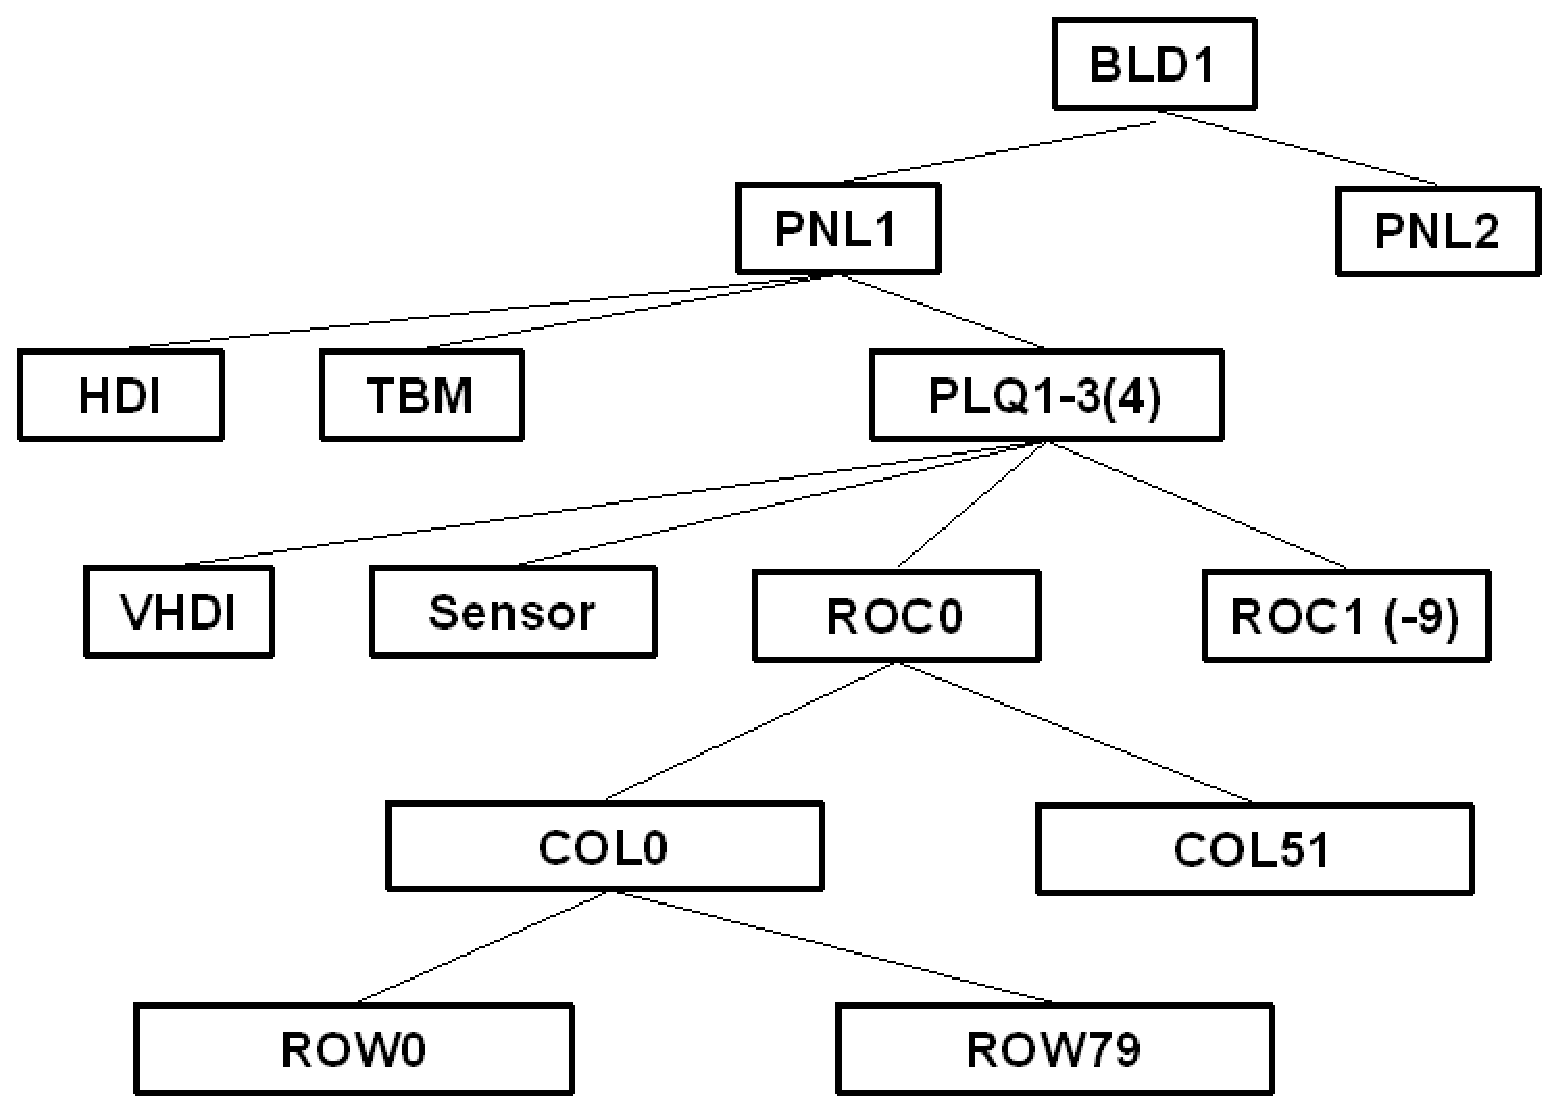
\includegraphics[width =0.7\textwidth]{Bld.eps}  
    \caption{Breakdown of the major components of a blade.}  
    \label{figure:bld}  
  \end{center}  
\end{figure}  

%The ROC also receives power (low voltages) for the digital and analog sections
%and the sensor receives a ``bias voltage''. These voltages are provided from
%CAEN power supplies that are ultimately controlled through the DCS system. 
%The organization and naming of these is described below.

The extension of the naming convention 
to cover the supporting electronics and power supplies
is described in the next few sections.


\subsubsection{Names for Token Bit Managers (TBMs)}

On each panel there is one TBM mounted,
which manages the data readout for all the ROCs mounted on the panel and handles
the communication for controlling the ROCs. 
The naming convention for the TBM is related to the panel on which it is mounted:
$\mbox{FPix\_B(p,m)(I,O)\_D(1-3)\_BLD(1-12)\_PNL(1,2)\_TBM.}$
The TBM itself is configured by several registers.
The names for these registers are of the form:
\begin{displaymath}
\mbox{FPix\_B(p,m)(I,O)\_D(1-3)\_BLD(1-12)\_PNL(1,2)\_TBM-REGNAME},
\end{displaymath}
where ``REGNAME'' is the name of one of the TBM registers,
a complete list of which is given in section~\ref{app:tbm} of the appendix.

The TBM receives commands from a particular PixelFEC, 
which is a VME module in the Control Room,
and routes them to the correct ROC. 
This requires the association of a VME address and various
PSI$^{2}$C addresses with the TBM. 
The association requires reference to some configuration tables, 
which are foreseen to be stored in the Configuration Database.
The exact mechanism is described in more detail below.
 The naming convention provides all the information
required to locate the configuration information in the database
that is needed to establish the communications link.

Each TBM reads out a panel and drives one optical fiber that goes to 
one channel of a VME Board, called a FED, of the front end electronics. 
The TBM and its
panel are associated with a particular Port Card and its Analog-Opto Hybrid
(AOH) which drives the optical fiber. The connection between the TBM and the
AOH is hardwired into the Adapter Board and its cabling to the Port Card.
Thus, one can think of either the AOH or the TBM as associated with 
a particular input to a channel of a FED board. This will be discussed below.


\subsubsection{Electronics for Half-Cylinders, Half-Disks, and Blades}

The detector components on a half-cylinder are organized half-disk wise.
Each half-disk includes several types of electronics cards and the chips
mounted on those cards, 
together with connection points for high voltages and low voltages, 
and RTDs used to monitor various temperatures on the half-disk. 
The electronics cards that serve half-disks are labeled as D1, D2 (and D3)
\footnote{There are two disks (D1 and D2) in current on-construction configuration. 
          The third disk is a possible upgrade.}, 
corresponding to the half-disk they belong to.
Table~\ref{table:on-detector:disk} lists the names of all the components 
of one particular half disk and their numbering. 
As shown in the table, each half-disk contains 12 blades (BLD), 
4 Adapter Boards (ADP), 4 Port Cards (PRT), 
high and low voltage channels and cooling channels.

  \begin{table}[htb]
    \caption{Numbering of on-detector components for the half-disk of the Forward Pixel detector
             installed close to the interaction point in +z direction on the side facing the center of the LHC ring with respect to the y-z plane (BpI).}
    \label{table:on-detector:disk}
%\small
    \begin{center}
      \begin{tabular}{l|ccccc|cc|cc} \hline
        Half-cylinder&         
        BLD&                 
        ADP&                 
        PRT&                 
        LV (blades)&                 
        LV (Port Card)&                 
        \multicolumn{2}{c|}{HV}&                 
        \multicolumn{2}{c}{Cooling}\\\hline


        \multirow{12}*{FPix\_BpI\_D1} &
        1&
        \multirow{3}*{1}&
        \multirow{3}*{1}&
        \multirow{3}*{1}&
        \multirow{12}*{1}&
        \multirow{3}*{1}&
        B1&
        \multirow{6}*{1}&
        In\\


        &
        2&
        &
        &
        &
        &
        &
        &
        &
        \\


        &
        3&
        &
        &
        &
        &
        &
        B2&
        &
        \\


        &
        4&
        \multirow{3}*{2}&
        \multirow{3}*{2}&
        \multirow{3}*{2}&
        &
        \multirow{3}*{2}&
        B1&
        &
        \\


        &
        5&
        &
        &
        &
        &
        &
        &
        &
        \\


        &
        6&
        &
        &
        &
        &
        &
        B2&
        &
        Out\\


        &
        7&
        \multirow{3}*{3}&
        \multirow{3}*{3}&
        \multirow{3}*{3}&
        &
        \multirow{3}*{3}&
        B1&
        \multirow{6}*{2}&
        In\\


        &
        8&
        &
        &
        &
        &
        &
        &
        &
        \\


        &
        9&
        &
        &
        &
        &
        &
        B2&
        &
        \\


        &
        10&
        \multirow{3}*{4}&
        \multirow{3}*{4}&
        \multirow{3}*{4}&
        &
        \multirow{3}*{4}&
        B1&
        &
        \\


        &
        11&
        &
        &
        &
        &
        &
        &
        &
        \\


        &
        12&
        &
        &
        &
        &
        &
        B2&
        &
        Out\\\hline


        \multirow{12}*{FPix\_BpO\_D1} &
        1&
        \multirow{3}*{5}&
        \multirow{3}*{5}&
        \multirow{3}*{5}&
        \multirow{12}*{2}&
        \multirow{3}*{5}&
        B1&
        \multirow{6}*{3}&
        In\\


        &
        2&
        &
        &
        &
        &
        &
        &
        &
        \\


        &
        3&
        &
        &
        &
        &
        &
        B2&
        &
        \\


        &
        4&
        \multirow{3}*{6}&
        \multirow{3}*{6}&
        \multirow{3}*{6}&
        &
        \multirow{3}*{6}&
        B1&
        &
        \\


        &
        5&
        &
        &
        &
        &
        &
        &
        &
        \\


        &
        6&
        &
        &
        &
        &
        &
        B2&
        &
        Out\\


        &
        7&
        \multirow{3}*{7}&
        \multirow{3}*{7}&
        \multirow{3}*{7}&
        &
        \multirow{3}*{7}&
        B1&
        \multirow{6}*{4}&
        In\\


        &
        8&
        &
        &
        &
        &
        &
        &
        &
        \\


        &
        9&
        &
        &
        &
        &
        &
        B2&
        &
        \\


        &
        10&
        \multirow{3}*{8}&
        \multirow{3}*{8}&
        \multirow{3}*{8}&
        &
        \multirow{3}*{8}&
        B1&
        &
        \\


        &
        11&
        &
        &
        &
        &
        &
        &
        &
        \\


        &
        12&
        &
        &
        &
        &
        &
        B2&
        &
        Out\\\hline




      \end{tabular}
    \end{center}
  \end{table}


%\begin{figure}[hbtp]
%  \begin{center}
%\includegraphics[width =0.8\textwidth]{Diskgroup.eps}
%    \resizebox{5cm}{1cm}{\includegraphics{cmslogo.eps}}
%    \caption{Components included in a half-disk group.}
%    \label{figure:disk}
%  \end{center}
%\end{figure}


Within a half-cylinder, there are some other miscellaneous components 
that are not associated with  half-disk 
groups, e.g on-shield RTDs. Another 
very important device in this category is the CCU Mother Board (CCUM board).
It houses the CCU chip and the DOH (Digital-Opto Hybrid) chips that
handle the standard I$^{2}$C controls communications between the control room and the electronics cards.
There is one  CCUM board for each half-cylinder. 
Figure~\ref{figure:bp} shows a block organization 
of the detector components for a  half-cylinder of the Forward Pixel 
detector.


\begin{figure}[hbtp] 
  \begin{center} 
        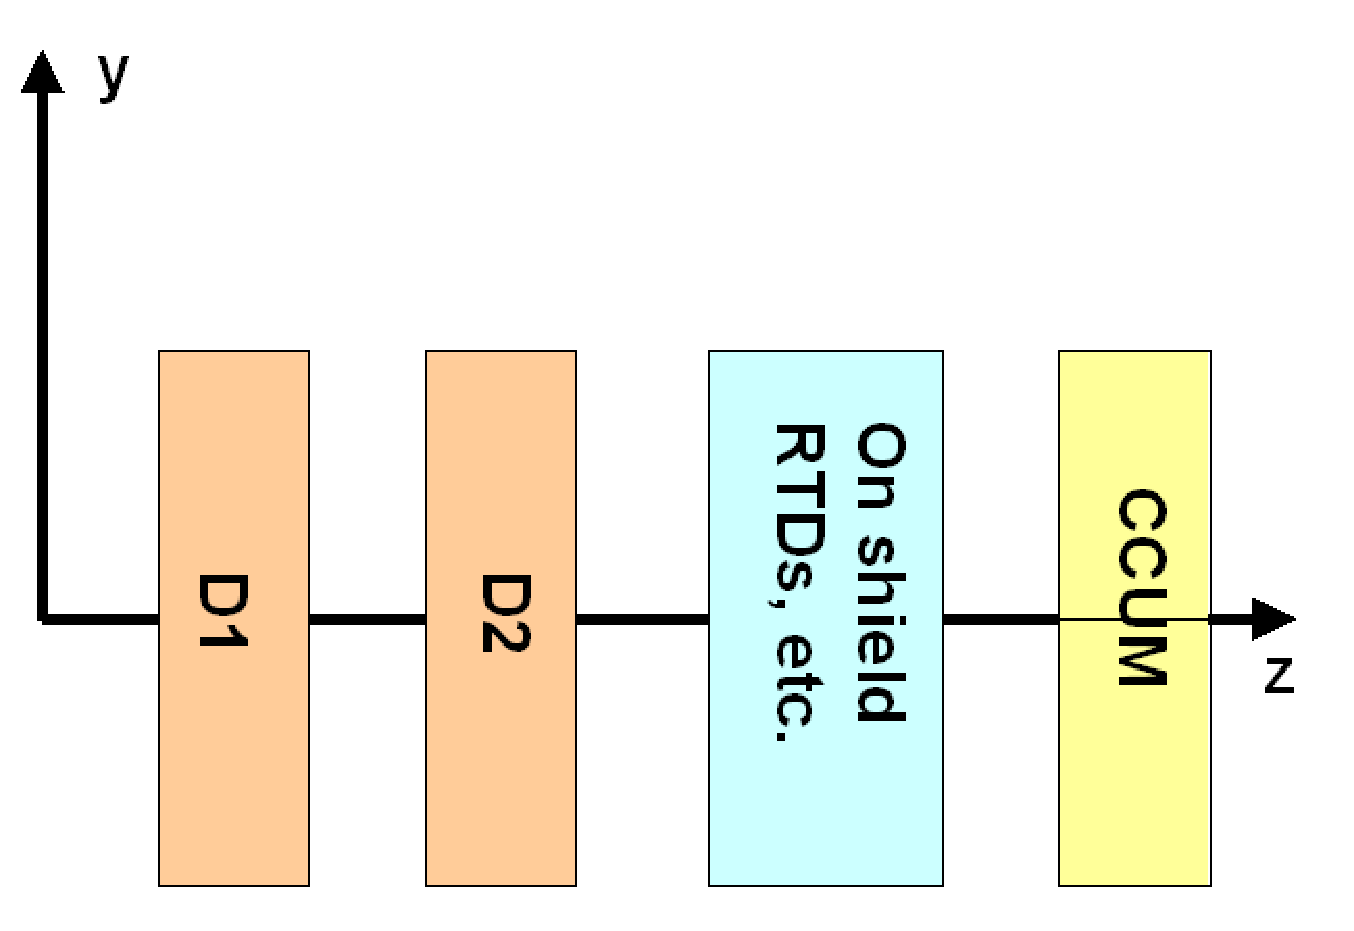
\includegraphics[width =0.6\textwidth]{Bp.eps} 
    \caption{Block of components for a  half-cylinder of the 
Forward Pixel detector.} 
    \label{figure:bp} 
  \end{center} 
\end{figure} 
 




\subsubsection{Names for a  Port Card and its Devices}

The Port Card (PRT) is essentially the communications interface between the  
pixel detectors and the electronics in the Control Room (US5). 
For each half-disk, there are 4 Port Cards mounted in a half-cylinder.
The Port Cards are distributed in azimuthal direction.
Each serves a group of three blades, 1-3, 3-6, 7-9, and 10-12, respectively. 
Following the convention on numbering azimuthally distributed devices, 
the Port Cards are numbered from 1 to 4. 
The names of the Port Cards are of the form:
$\mbox{FPix\_B(p,m)(I,O)\_D(1-3)\_PRT(1-4).}$. 

A Port Card contains the following chips to fulfill its quite complex tasks 
in the detector operation:
\begin{itemize}
\item one Detector Control Unit (DCU). 
\item one Digital-Opto Hybrid (DOH), which contains: 
\begin{itemize}
\item two Laser Diodes (LSR) and 
\item one Linear Laser Driver (LLD).
\end{itemize}
\item one Tracker Phase-Locked Loop (PLL). 
\item one Delay 25 (DEL). 
\item one Gate Keeper (GTK).
\item one Analog-Opto Hybrid (AOH) board, which contains two LLDs and two 
Analog Level Shifter (ALT) chips. The AOH board drives 6 optical signals 
on 6 optical fibers, one for each panel of the three blades.
\item one Resistance Temperature Detector or  RTD (RTD).. 
\end{itemize}

Figure~\ref{figure:prt} shows a block diagram of a Port Card,
together with the names used to identify each of its major components. 

\begin{figure}[hbtp]   
  \begin{center}   
        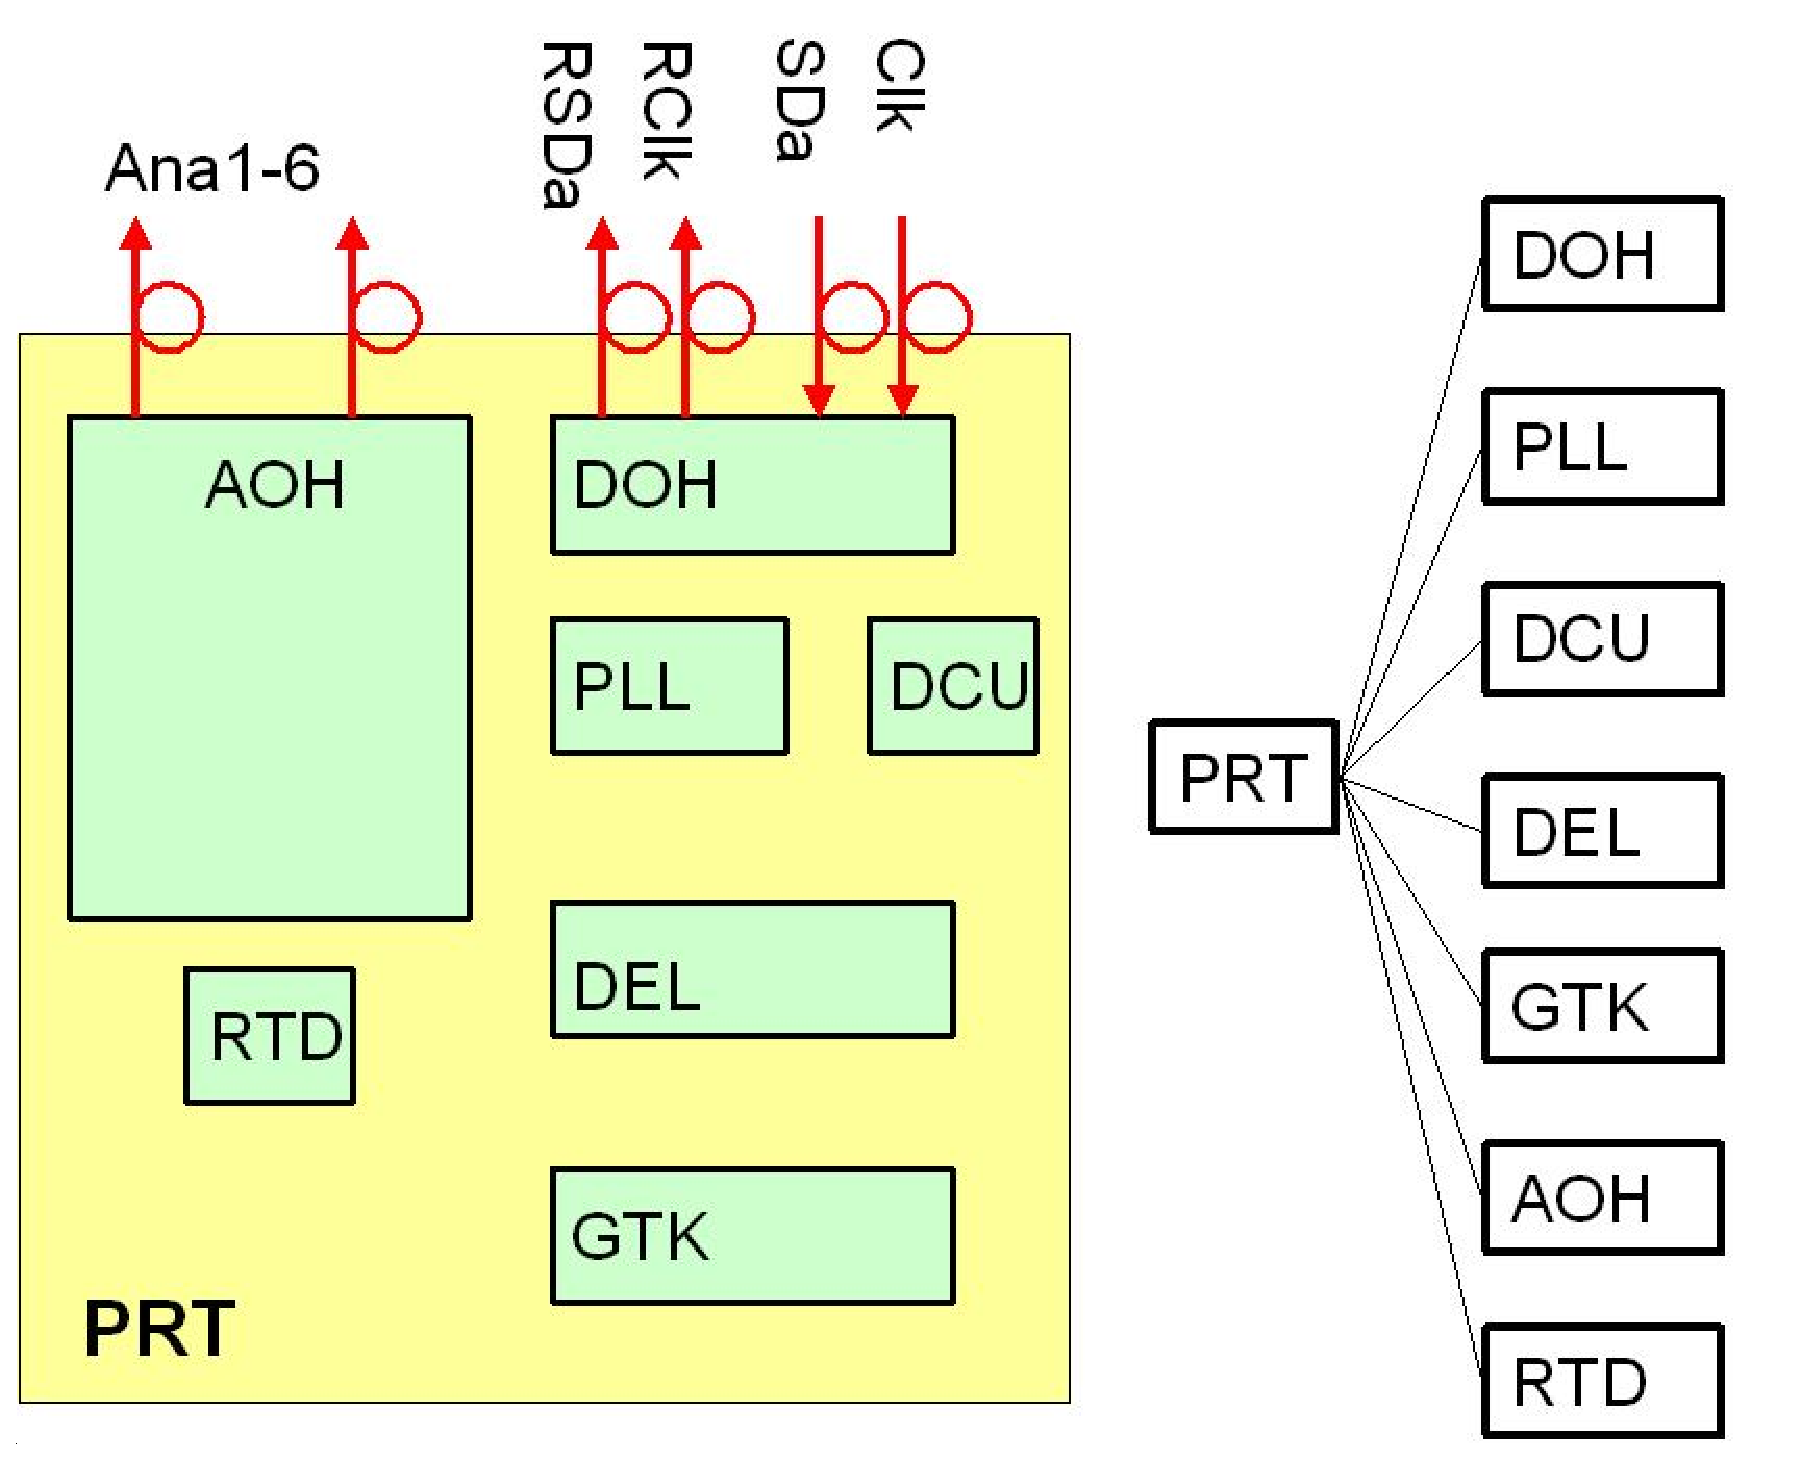
\includegraphics[width =0.7\textwidth]{prt_v1.eps}   
    \caption{Breakdown of the major components for a Port Card (PRT).}   
    \label{figure:prt}   
  \end{center}   
\end{figure}  

The names of the DCU, DOH, PLL, DEL and GTK chips
and of their registers is related to the Port Card on which they are mounted
and are of the form:
$\mbox{FPix\_B(p,m)(I,O)\_D(1-3)\_PRT(1-4)\_DCU\_REGNAME}$.
The complete list of registers of the DCU, DOH, PLL, DEL and GTK chips
is given in sections \ref{app:lld}-\ref{app:dcu} of the appendix. 
The Gate Keeper has no readable or writable registers.
We decided to give it  a name nonetheless.

The AOH board on a Port Card is named
$\mbox{FPix\_B(p,m)(I,O)\_D(1-3)\_AOH(1-4)}$.
Each AOH has 6 optical output channels that are numbered 1-6 and identified by:
$\mbox{FPix\_B(p,m)(I,O)\_D(1-3)\_AOH(1-4)\_ANA(1-6)}$.
The light output of the optical channels on the AOH board
can be controlled by programmable registers.
The complete list of registers of the LLD and ALT chips mounted on the AOH boards
is given in section \ref{app:lld} and \ref{app:alt} of the appendix.

%Since there is only one of each chip on a Port Card, 
%the AOH, PLL, DEL, DCU and DOH on
%each Port Card, we prefer to treat these as azimuthally distributed
%devices independent of the Port Card.
%Following this convention, the AOH on a port 
%card of the Forward Pixel detector can be named as, 
%$$\mbox{FPix\_B(p,m)(I,O)\_D(1-3)\_AOH(1-4)}$$.
%Each AOH has 6 optical output channels numbered 1-6. The channels
%are defined ANA and their full address is:
%$$\mbox{FPix\_B(p,m)(I,O)\_D(1-3)\_AOH(1-4)\_ANA(1-6)}$$.
%The AOH also has programmable registers that control the gain and bias of
%the outputs.  The names of the registers are given in the appendix.
%An example of a name of an AOH register is
%$$\mbox{FPix\_B(p,m)(I,O)\_D(1-3)\_AOH(1-4)\_ANA(1-6)-GAIN(0-1)}$$.
%
%The PLL, DEL (Delay25), and DOH  are also indexed from 1-4 based on the convention for azimuthally distributed devices. It is evident
%that the Port Card associated with any of these devices in azimuthal 
%position $i$ is the Port Card in with the same index in that half-cylinder.
%
%We also give the GateKeeper a name, GTK, and an index (1-4) even though 
%it has no readable or writable registers.
%
%The optical inputs and outputs for the DOH are named as 
%Clk, SDA, RClk, and RDSa.
%
%Finally, the Port Card also receives power for its own chips and provides 
%two different Low Voltages  to the Adapter Board, which passes them onto
%the panel where they power the TBM and the ROCs.
%These voltages originate from CAEN power supplies in the
%Control Room over cables that run through boards called Power Distribution 
%Boards, discussed below. These supply tie points in the CCUM  that will
%also be given names.


\subsubsection{CCUM boards}

There is one CCUM board for each half-cylinder. 
For this reason, the CCUM board does not require a number 
(since the number would always be 1).
Each CCUM interfaces to all 8 Port Cards (four on each half-disk)~\footnote{In case a third half-disk gets installed in each half-cylinder 
in a future upgrade of the Pixel detector, each CCUM interfaces to 12 Port Cards.} 
in its half-cylinder. 
Each CCUM board contains 4 CCU chips.
The CCU chips contain a I$^2$C ``node controller'' that manages
the communication of a single I$^2$C port.
The CCU chips are named CCU(1-4).
While the hardware issues here are very complex, the result is simple:
CCUi controls  the Port Card PRTi for all three disks of the half-cylinder.
This means that one CCU provides control for I$^{2}$C devices of an entire
$\phi$ slice of 45$^{\circ}$ including all three half-disks.
In addition, each CCUM board contains 2 DOH chips that receive the control commands
from the Tracker FEC via optical fibers.

\begin{figure}[hbtp]   
  \begin{center}   
        \includegraphics[width =0.65\textwidth]{new_CCU_v1.eps}   
    \caption{Breakdown of the major components for a CCUM board.}   
    \label{figure:ccum}   
  \end{center}   
\end{figure} 

As we did for the Port Cards, we further break down the major components of the CCUM boards.
The major components of the CCUM board are depicted in figure~\ref{figure:ccum}.
The 4 CCU chips on the CCUM board can be identified as:
$\mbox{FPix\_B(p,m)(I,O)\_CCUM\_CCU(1-4).}$
The two DOH chips are named DOHa and DOHb:
$\mbox{FPix\_B(p,m)(I,O)\_CCUM\_DOH(a,b).}$
Each DOH chip has two optical inputs and two optical outputs; 
Clk, SDA, RClk, and RDSa; which may be referenced as:
$\mbox{FPix\_B(p,m)(I,O)\_CCUM\_DOH(A,B)-(Clk, SDA, RClk, RDSa).}$

The association between devices on Port Cards (DCU, DOH, PLL, DEL, GTK and AOH)
and the CCU port and its I$^2$C channels can be accessed via a small  
table in the Configuration Database.

%The CCUM card itself also receives low voltages from CAEN power supplies in the
%Control Room over cables that run through boards called Power Distribution 
%Boards, discussed below. These supply tie points in the CCUM that will
%eventually also be given names.


\subsubsection{Adapter Boards, Low Voltage Connections, and
Bias Voltage Connections \label{sec:adp}}

Adapters Boards connect sets of three blades on one Port Card. 
The Adapter Boards have no programmable registers or readable elements. However, we do provide
a name for them, ADP(1-4), 
with the number in parentheses corresponding to the Port Card to which that the Adapter Board connects to,
as the Adapter Boards serve as high voltage connection points, 
providing bias voltage for the sensors on the 6 Panels connected to the Adapter Board.
For each Adapter Board, there exist actually two separate high voltage channels,
one to supply the bias voltage for the sensors of the ``inner'' plaquettes (the ones closest to the beam line)
\footnote{On four plaquette panels, the ``inner'' plaquettes are the 1x2 and the 2x3 plaquettes,
          while on three plaquette panels there is only one ``inner'' plaquette, the plaquette of type 2x3.
          The ``outer'' plaquettes are the 2x4 and 1x5 ones on four plaquette panels,
          while being the 2x4 and 2x5 types on three plaquette panels.}
and one to supply the bias voltage for the sensors of the ``outer'' plaquettes (the ones furthest apart from the beam line).
The splitting into inner and outer plaquettes is done to account for the fact that the plaquettes closer to the beam line
will receive a higher radiation dose than those further apart,
so may need to operate at a higher bias voltage.
The two bias voltages are labeled ``I'' for inner
group (smaller radius) and ``O'' for outer group (larger radius). 
In addition, we give these voltages (actually the connectors on the Adapter Boards) numbers from 1-4,
corresponding to the number of the Port Card the Adapter Board is connected to.
The names for a high voltage connection are thus of the form:
$\mbox{FPix\_B(p,m)(I,O)\_D(1-3)\_HV(1-4)(I,O).}$

Each Port Card/Adapter Board also supplies two ``low voltages'' to the ROCs.
One provides power to the analog sections of the chip and the other to the digital
section of the chip. These are further adjusted by on-chip voltage regulators
call ``VANA'' and ``VDIG,'' respectively. We refer to the connection points
for these as LV(1-4) for the four adapter board/port card/octants and (A,D) for the
analog section supply voltage or the digital section supply voltage.
The names for a low voltage connection are thus of the form:
$\mbox{FPix\_B(p,m)(I,O)\_D(1-3)\_LV(1-4)(A,D).}$

%% not sure this is consistent. does this have a value or is it just
%% an end point to attach the DCS channel value to?
%% what about HV4-o, HV4-i, or even ADP4-HVo, ADP4-HVi? 


\subsubsection{Quadrants}

The temperature of cooling channels are monitored by the DCS system. 
Since the cooling channels are organized into loops that span 1/4 of a cylinder, 
it is useful to provide a name for quadrants: Q1, Q2, Q3, and Q4, following 
the numbering rules for azimuthally distributed detectors. The quadrant is 
specified for a device only if it cannot be deduced from other elements of 
the name hierarchy. For example, if the blade number appears in the name, the 
quadrant is not specified since it can be deduced from the blade number.

\subsubsection{$\phi$ Sectors}

For the purpose of describing the detector control network,
it is useful to think of the 45$^{\circ}$ slice in azimuthal angle covered by three blades and extending to two (three) disks as a single unit.  For each 
half-cylinder, the sector numbers run from 1-4, from the top to the bottom:
SEC(1-4).

SEC(i) contains PRTi and ADPi and all their components for D1, D2, and D3( when
it is implemented).


\subsubsection{Filter Boards}

For distributing the high and low voltages for the analog and digital parts of the ROCs,
for the TBM and for the electronics mounted on the Port Cards and CCUM boards,
additional boards are installed near the end-flange of each half-cylinder.
These so-called Power Filter Boards distribute the power coming from the CAEN power supplies
in the galley to the individual components that need them.
Other boards are installed near the end-flange of each half-cylinder that fanout
the connections coming from multi-conductor control cables to individual RTDs 
and HMX humidity sensors of the DCS system.

There are three types of Filter Boards:
\begin{enumerate}
\item The Power Filter Board Type A (PFA) distributes Low Voltage DC power 
through the Adapter Board to the ROCs and TBMs
and bias voltage to the pixel sensors for the three blades served by one Port Card/Adapter Board. Each PFA
receives one so-called Multi-Service cables that carry all the required voltages. There are twelve PFA's per 
half-cylinder. The naming scheme for these boards takes advantage of the their association with specific
adapter boards:
$\mbox{FPix\_B(p,m)(I,O)\_D(1-3)\_ADP(1-4)}$.
\item The Power Filter Board Type P (PFP) provides Low Voltage DC Power to the Port Cards and (single) CCUM of
of a half cylinder. A single so-called Auxiliary Power Cable comes into the PFP. The naming scheme for
a PFP is $\mbox{FPix\_B(p,m)(I,O)\_PFP}$.
\item The Sensor Filter Board (SFS) provides twisted pairs to carry signals from RTDs and humidity
sensors to the Analog-to-digital converters of the slow control system. There are two SFS boards 
per half-cylinder. Each SFS Board receives one so-called Sensor cable. The naming scheme for
the SFS boards is $\mbox{FPix\_B(p,m)(I,O)\_Q(1,2)\_SFS(1,2)}$. 
\end{enumerate}

The Filter Boards do not  have any programmable functions. 
However, they are given names according to the naming convention 
for completeness and also for possible inclusion in databases 
(e.g. cable connection databases, equipment inventory databases).


\subsubsection{Summary of the Physical Naming for On-detector Components}

\begin{figure}[hbtp]   
  \begin{center}   
        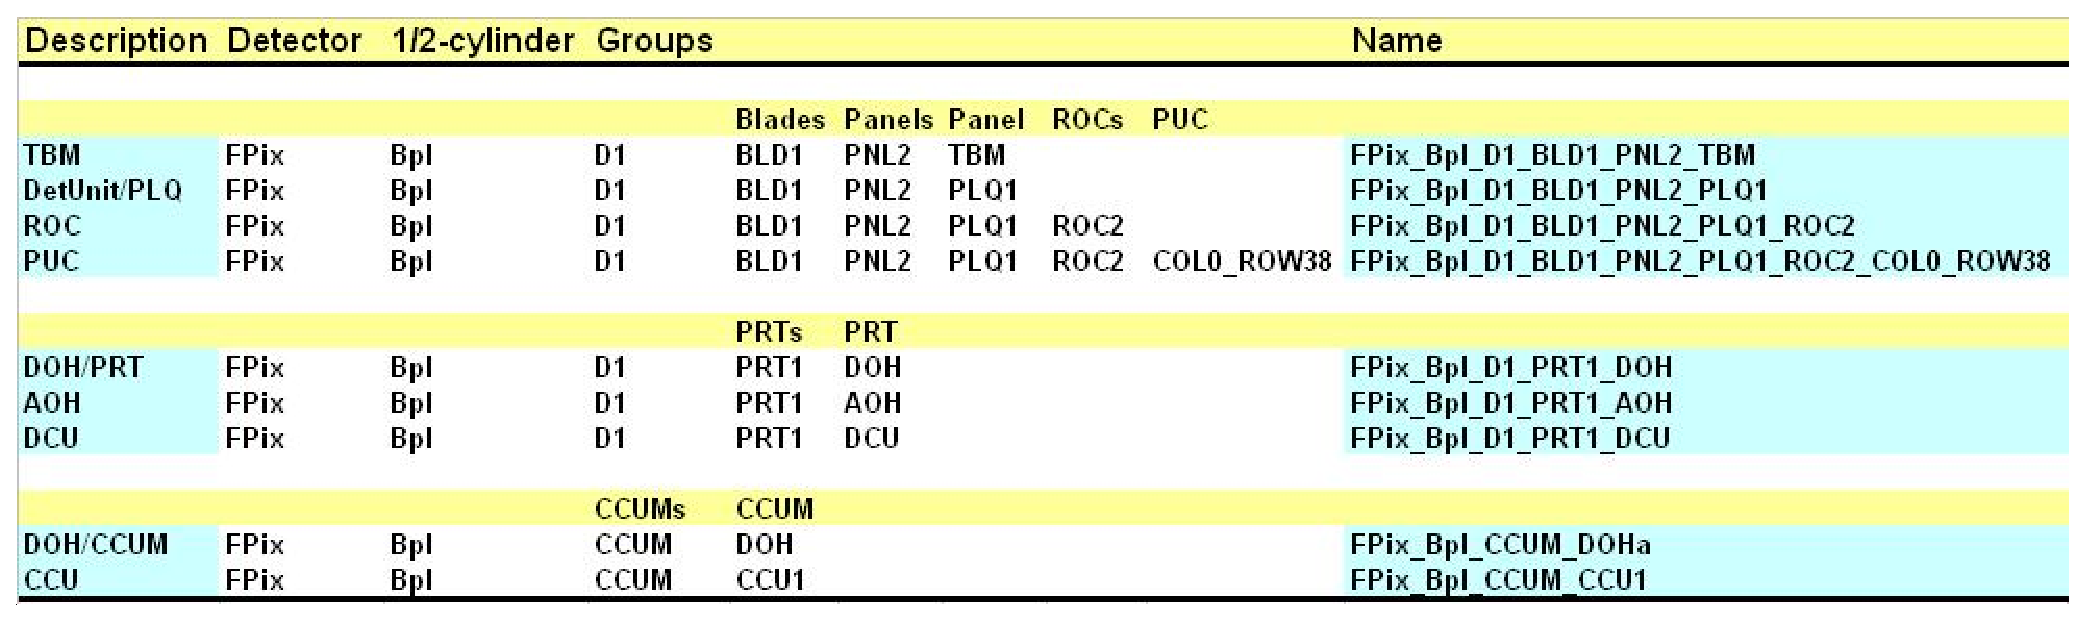
\includegraphics[width =0.95\textwidth]{summary_v1.eps}   
    \caption{Summary of physical naming convention for on-detector components. 
Examples are used to illustrate this convention. }
    \label{figure:summary}   
  \end{center}   
\end{figure} 

With the conventions described above, 
the names of on-detector components are fully defined.
As examples, names of some devices are given in figure~\ref{figure:summary}. 


\subsection{The Barrel Pixel System}

The BPix components are located in the CMS collision hall and in the control room. 
Similar to the components of the Forward Pixel detector,
they can be divided into control room electronics and on-detector components.

The Barrel pixel name hierarchy extends through several hierarchy levels, as described below.
%The full hierarchy to describe a pixel is:
%$\mbox{BPix\_B(p,m)(I,O)\_SEC(1-8)\_LYR(1-3)\_LDR((1H, 2F-(N-1)F,NH,)
%\_MOD(1-4)\_ROC(0-(7,15))\_COL(0-51)\_ROW(0-79).}$
%
%The individual elements of the hierarchy are described below.


\subsubsection{Shells}

The Barrel detector has a cylindrical structure co-axial to the beam and 
centered on the IP. It consists of three cylindrical layers. 
The layers are split into half-cylinders along the y-z plane.

The names of the Barrel Pixel on-detector components always start with 
BPix to distinguish them from those of the Forward pixel detector. 
The components on
the positive z-axis side and the negative z-axis side are prefixed with Bp 
and Bm, respectively. So there are 
two major groups of components: BPix\_Bp  and 
BPix\_Bm. On each side of the IP, the detector is composed of 
two half-cylinders, called 
Inside (I) and Outside (O) half-cylinders.
These four divisions are referred
to as ``shells'', defined and named as follows:
\begin{itemize}
\item  BPix\_BpI, at positive z and positive x; 
\item  BPix\_BpO, at positive z and negative x;
\item  BPix\_BmI, at negative z and positive x; and
\item  BPix\_BmO, at negative z and negative x.
\end{itemize}

Figure~\ref{figure:bpix_shells} shows the shell layout.

\begin{figure}[hbtp] 
  \begin{center} 
        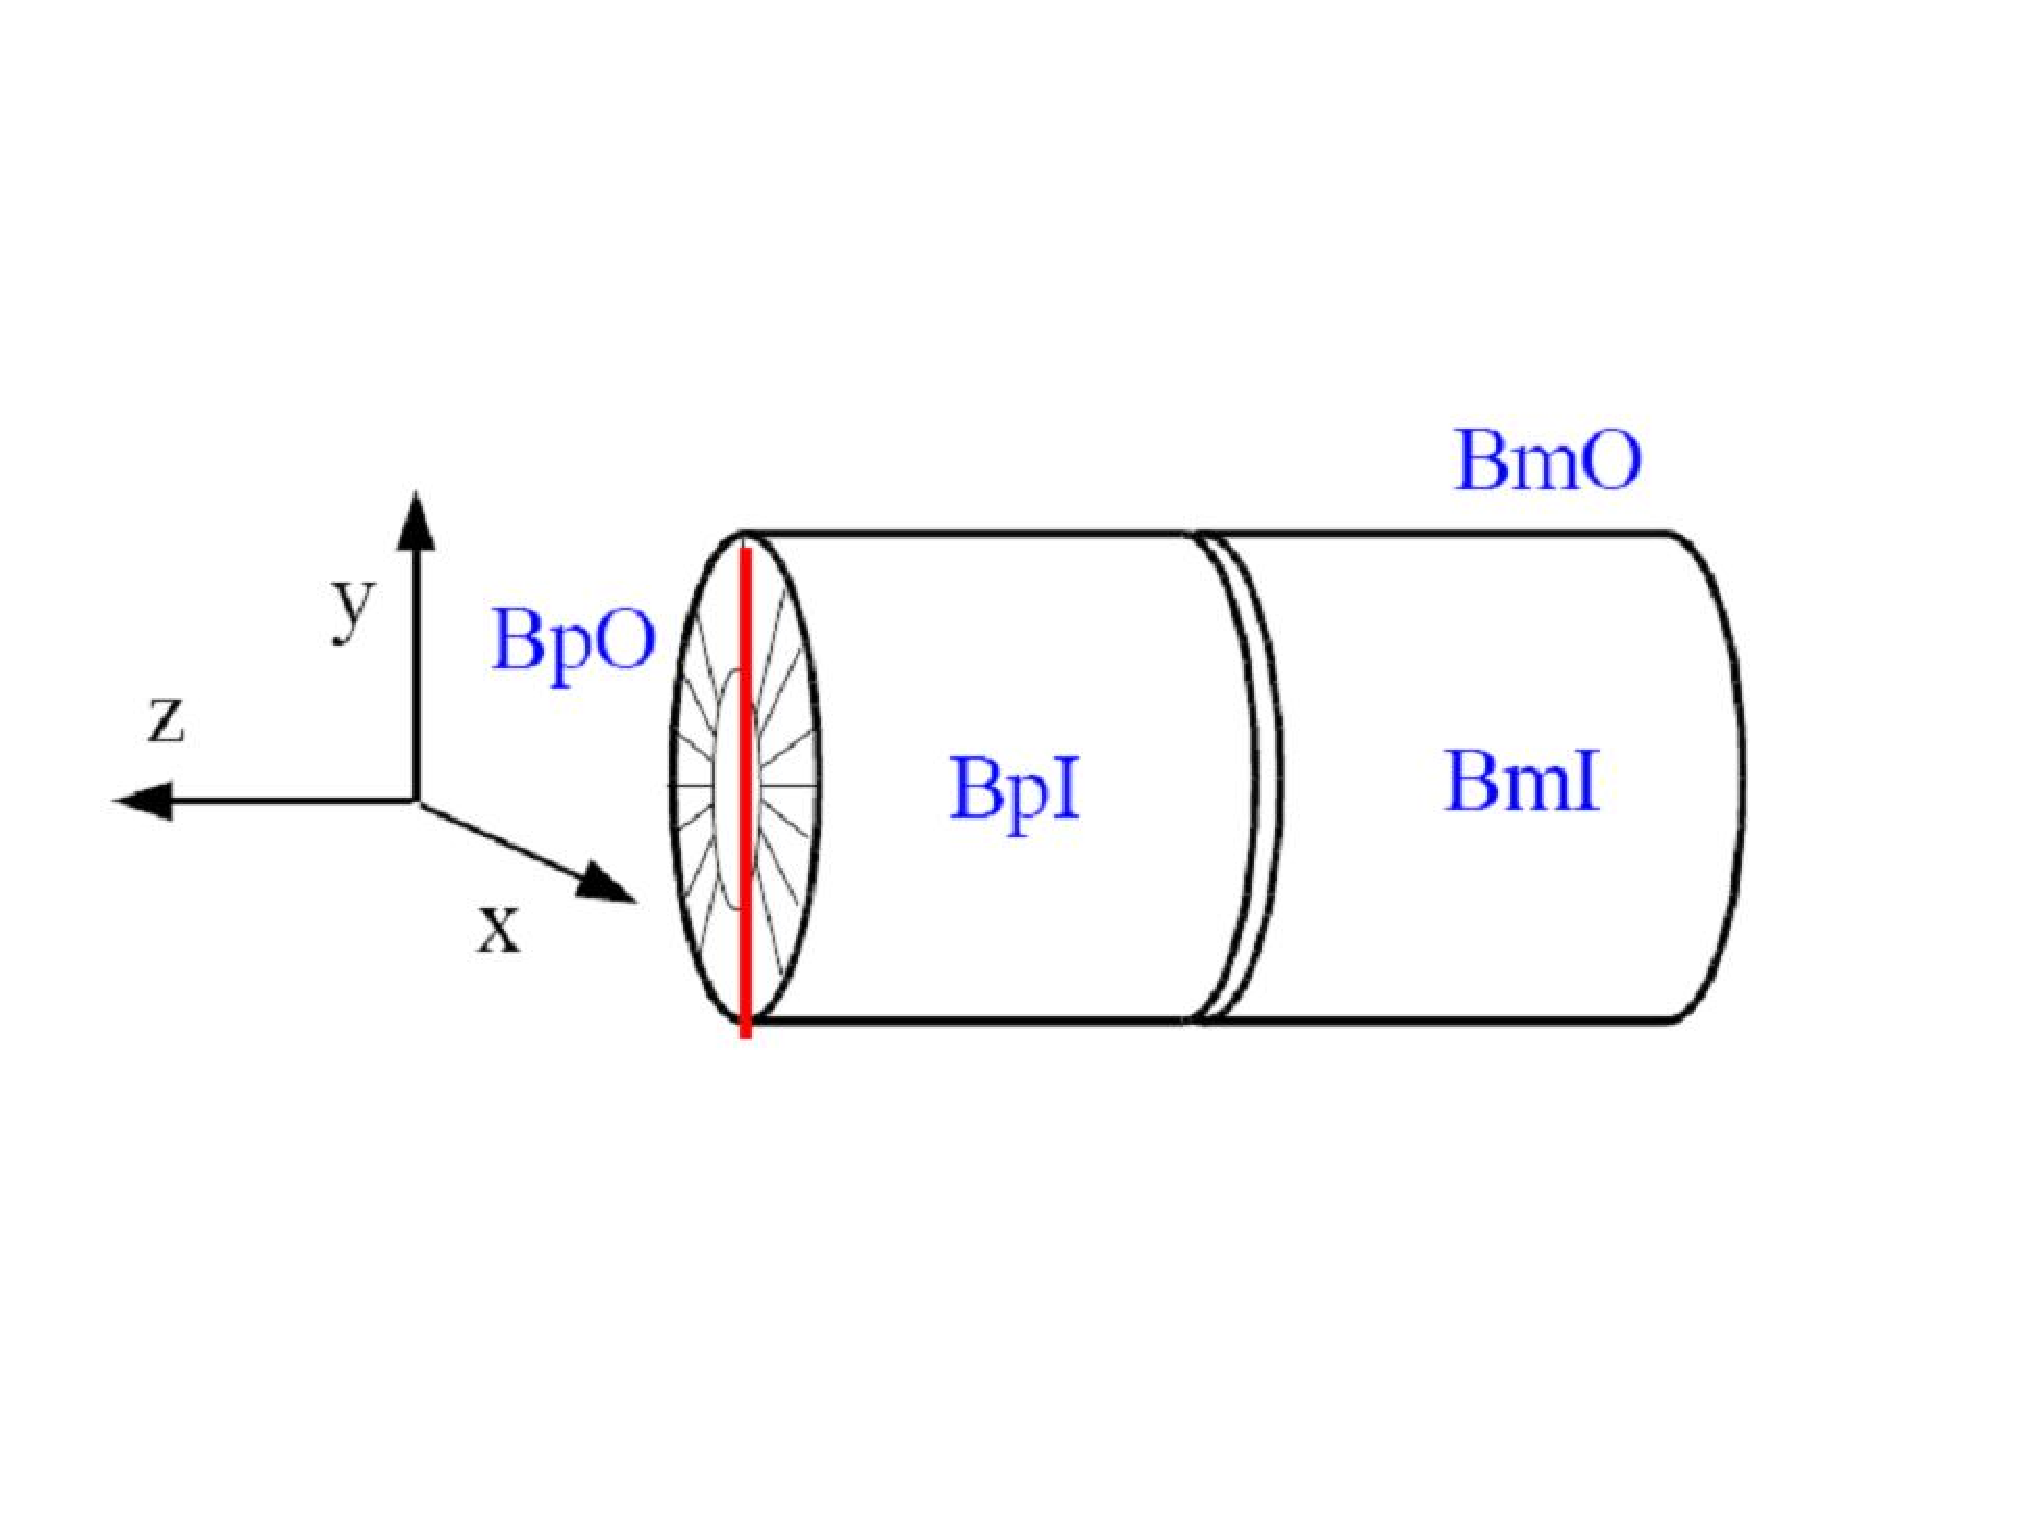
\includegraphics[width =0.6\textwidth]{barrel_z_seg.eps} 
    \caption{Schematic of Barrel Pixel Shells} 
    \label{figure:bpix_shells} 
  \end{center} 
\end{figure} 

\subsubsection{Sectors}

Shells are divided into 8 ``sectors.'' Each sector is an azimuthal slice
of a shell (and includes all three concentric cylinders). The sectors are 
numbered from 1 to 8 starting with 1 at the top
and continuing to 8 at the bottom.
A sector of a shell is named as:
$\mbox{BPix\_B(p,m)(I,O)\_SEC(1-8).}$


\subsubsection{Layers}

Each sector of a shell consists of three concentric cylindrical sections,
called ``layers''. 
The layers are numbered LYR(1-3), 
with 1 being the one closest to the beam axis. 
Specifically, the numbering is:
\begin{itemize}
\item LYR1 for the layer installed at a radius of 4 cm from the beam axis;
\item LYR2 for the layer installed at a radius of 7 cm from the beam axis; and
\item LYR3 for the layer installed at a radius of 11 cm from the beam axis.
\end{itemize}
The layers are named as:
$\mbox{BPix\_B(p,m)(I,O)\_SEC(1-8)\_LYR(1-3).}$


\subsubsection{Ladders}

Each layer of a sector of a shell consists of ``ladders'' (abbreviated as ``LDR'') of several modules
(described below) of pixel detectors. Since the layers have different
radii, they are covered by different numbers of ladders. Moreover,
because of symmetry issues at the vertical gap, there are two types of 
ladders, ``full-ladders'' and ``half-ladders.'' The half ladders of each
layer lie along the edges of the half-cylinder. The half-ladders are made of 
``half-modules'', which are the same length along z as ``full ladders'', 
but have only half the transverse width.

The number of ladders,
half and full, for each layer of each shell is:
\begin{itemize}
\item LYR1: 10 ladders (2 half-ladders and 8 full ladders);
\item LYR2: 16 ladders (2 half-ladders and 14 full ladders); and
\item LYR3: 22 ladders (2 half-ladders and 20 full ladders).
\end{itemize}

The ladders are numbered starting at 1 at the top and ending with 10, 16 or 22 
(for layers LYR1, LYR2 or LYR3) at the bottom.
In case the ladder is a half-ladder, 
the character ``H'' is appended to the number,
while for full ladders the character ``F'' is appended.
So, the two half-ladders in a particular layer of a shell are labeled 1H and NH,
where N denotes the number of ladders in that layer,
and the full ladders in between the half-ladders are numbered from 2F to (N-1)F.
Note that we number the ladders consecutively around the whole shell - that 
is, we do not restart the numbering from 1 at each sector boundary. This 
convention is derived from long-standing usage. 

The name of a ladder is thus of the form:
$\mbox{BPix\_B(p,m)(I,O)\_SEC(1-8)\_LYR(1-3)\_LDR(1H,2F-(N-1)F,NH),}$
where N=10, 16, 22 for layers LYR1, LYR2 and LYR3, respectively. 

The full numbering scheme for shells, sectors, and ladders is shown in
Fig.~\ref{figure:barrel_layout}. The naming hierarchy down to the level of the
ladder is shown in Fig.~\ref{figure:bpix_hier1}.

\begin{figure}
\begin{center}   
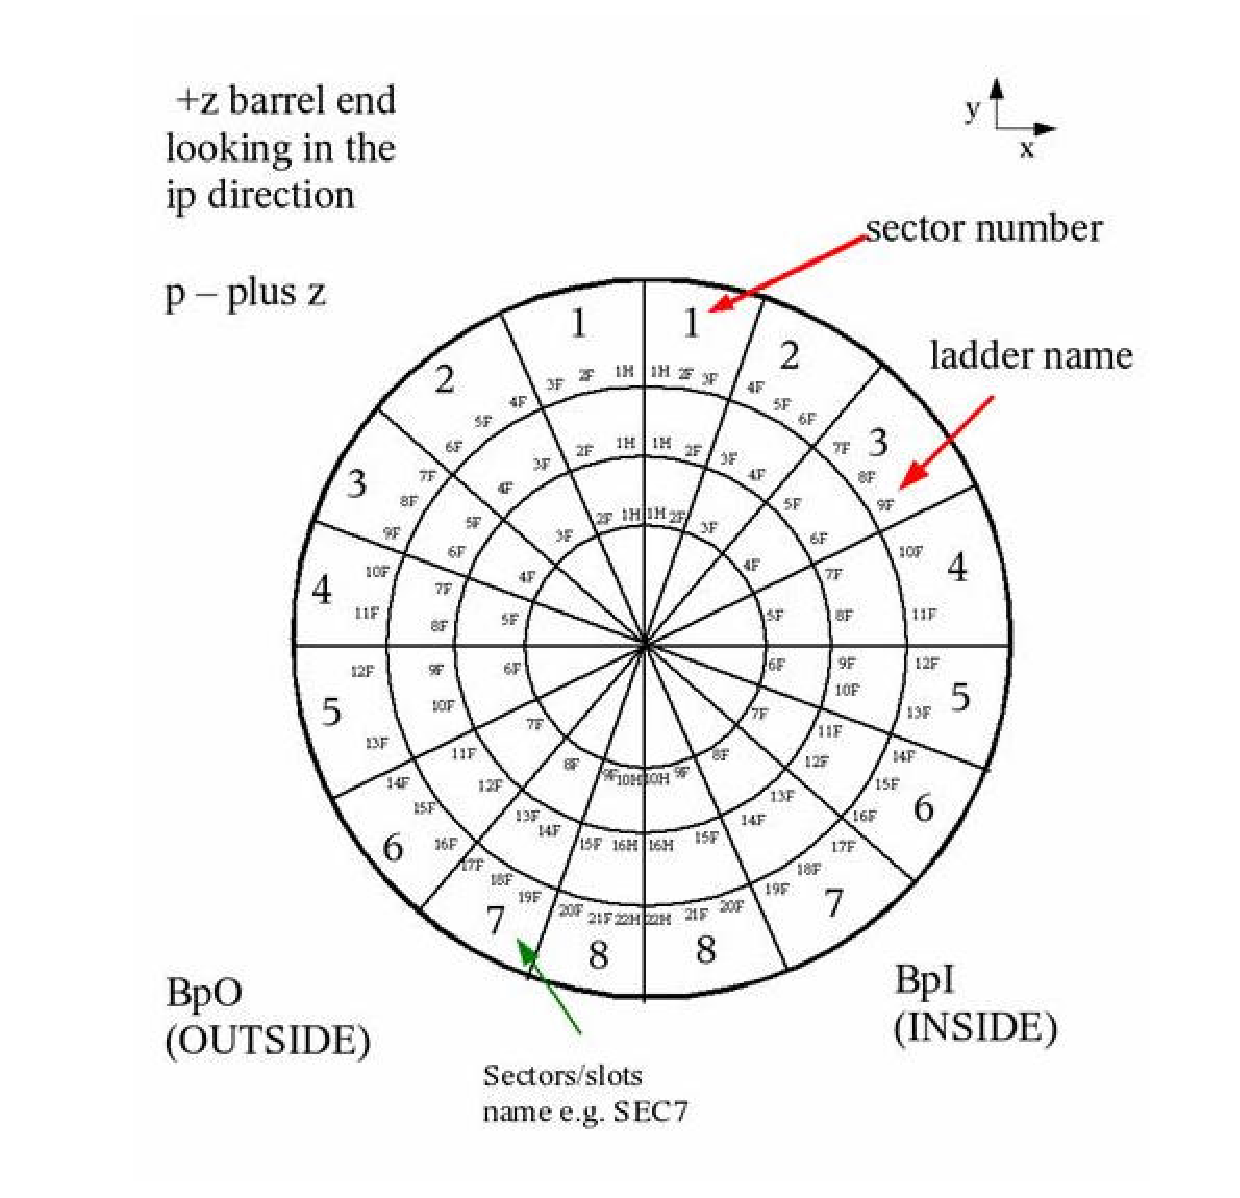
\epsfig{file = barrel_sector.eps, height = 100mm,
        bbllx=67, bblly=23, bburx=539, bbury=534, clip=}
%        bbllx=8, bblly=34, bburx=699, bbury=499, clip=}
%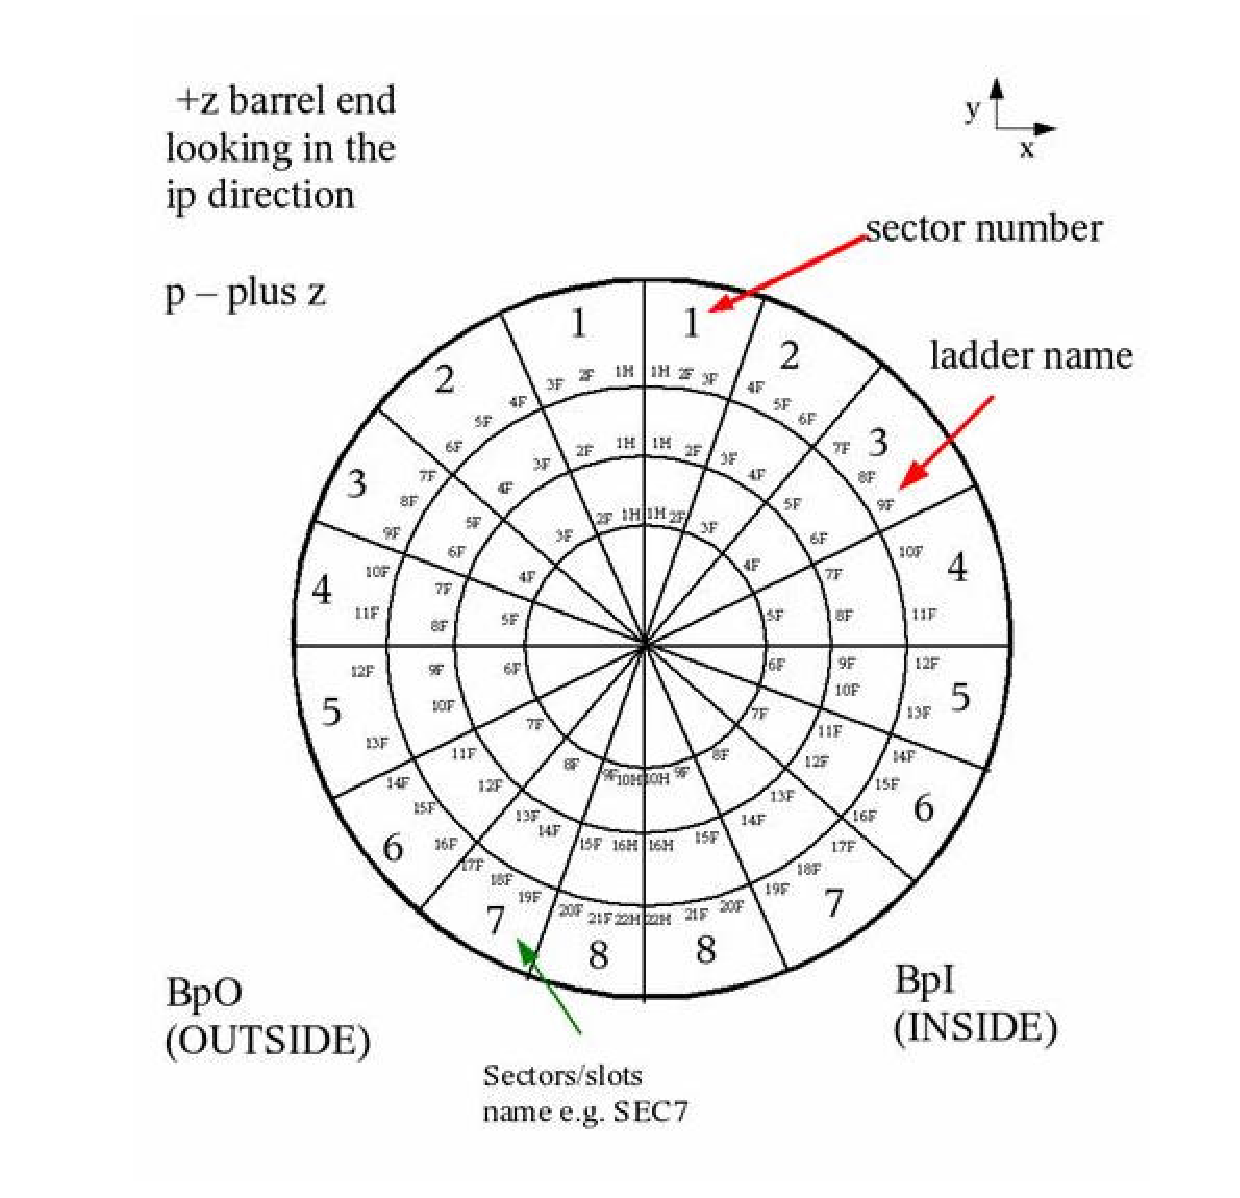
\includegraphics[width =0.9\textwidth]{barrel_sector.eps}   
\caption{Illustration of the Barrel Pixel detector showing the labeling
scheme for sectors, layers, and ladders.     
\label{figure:barrel_layout} }
\end{center}
\end{figure}

Note that the number of ladders varies among the different sectors of the layers. 
For Layer 1, there are two ladders, one half and one full, 
in the two sectors, 1 and 8, adjacent to the edge of the half-cylinder 
and one full ladder in the six other sectors, 2-7. 
For Layer 2, there are two ladders in every sector but the two in the sectors, 1 and 8,
adjacent to the edge of the half-cylinder contain one half-ladder and one-full ladder, 
while the other six sectors, 2-7, contain two full ladders.
For Layer 3, the two sectors, 1 and 8, that are adjacent to the half-cylinder edge,
have three ladders, one half-ladder and two full ladders; 
the two sectors adjacent to the x-axis, 4 and 5, each have two full ladders; 
and the remaining four sectors, 2, 3, 6, and 7, have three full ladders.

\begin{figure}[hbtp] 
  \begin{center} 
        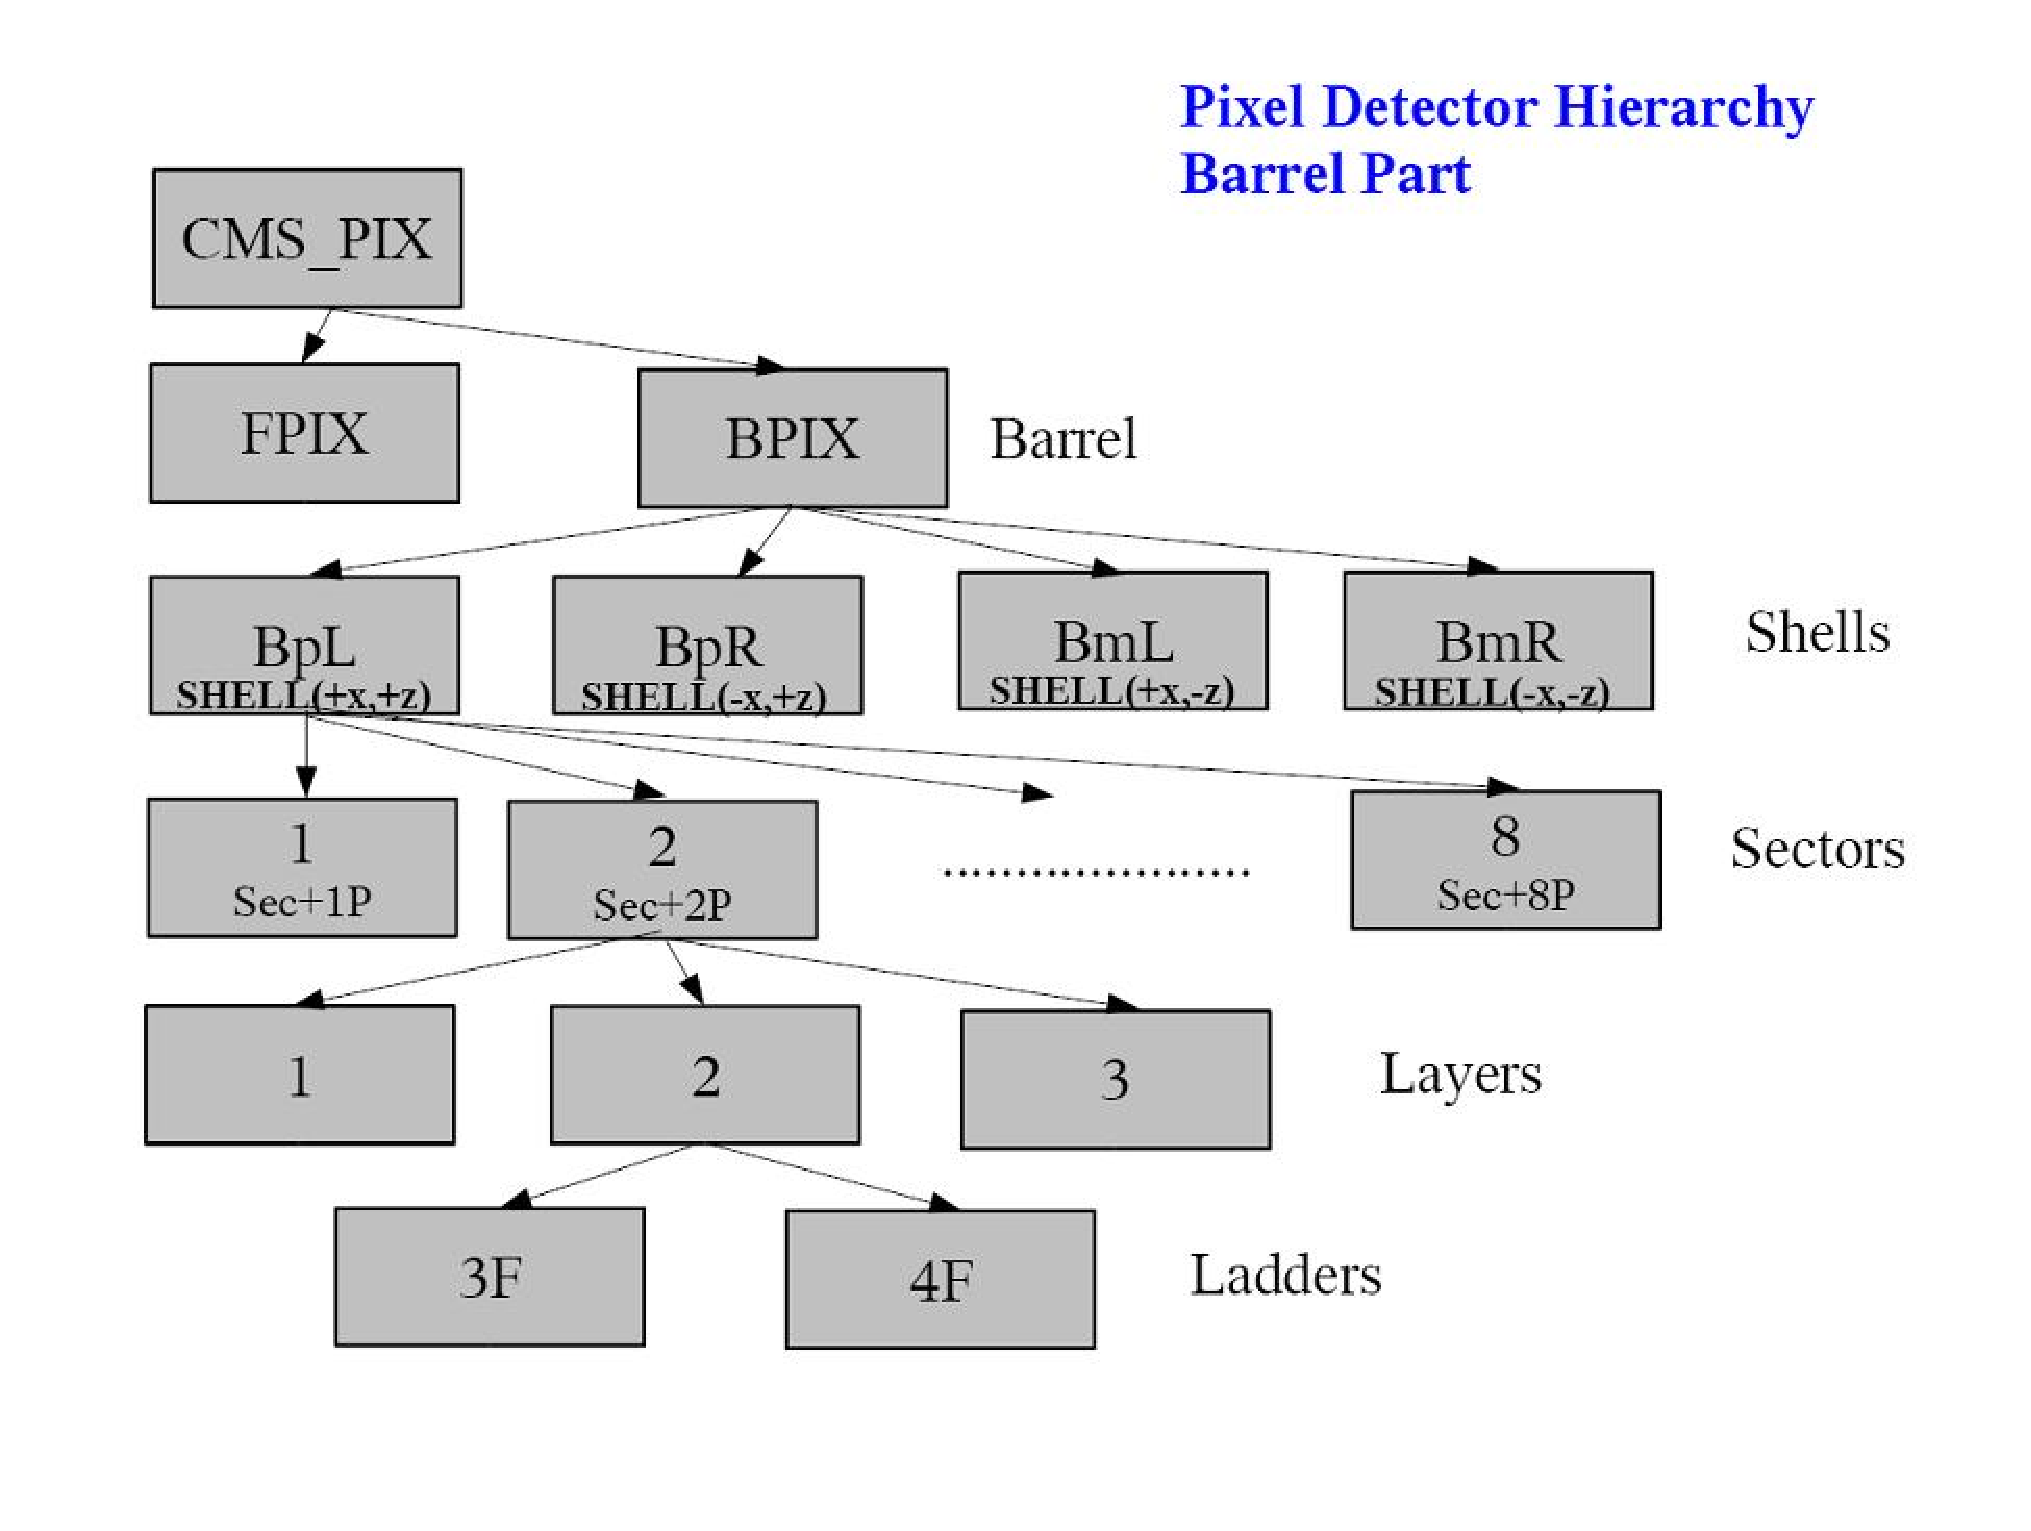
\includegraphics[width =0.6\textwidth]{barrel_hierarchy.eps} 
    \caption{Barrel pixel hierarchy down to the ladder.} 
    \label{figure:bpix_hier1} 
  \end{center} 
\end{figure} 

\subsubsection{Modules}

Each ladder is composed of four ``full modules'' or four ``half modules,''
depending on whether it is a full-ladder or a half-ladder. 
A full module consists of an 8x2 array of readout chips bonded to a pixel sensor. 
A half-module consists of an 8x1 array of readout chips bonded a pixel sensor half the size.
In either case, the long dimension of the module is aligned with the z-axis. 
Within a ladder, the modules are numbered from 1 to 4, 
with 1 being always closest to the IP and 4 being farthest from the IP.   

The names for modules is of the form:
\begin{displaymath}
\mbox{BPix\_B(p,m)(I,O)\_SEC(1-8)\_LYR(1-3)\_LDR(1H,2F-(N-1)F,NH)\_MOD(1-4).}
\end{displaymath}


\subsubsection{Readout Chip Number}

As in the Forward Pixel case, the readout chips are numbered 
according to the passage of the readout token issued by the TBM.

The names for the ROCs in the Barrel Pixel detector is of the form:
\begin{displaymath}
\mbox{BPix\_B(p,m)(I,O)\_SEC(1-8)\_LYR(1-3)\_LDR(1H,2F-(N-1)F,NH)
\_MOD(1-4)\_ROC(0-(7,15)),}
\end{displaymath}
where N is 15 for a full module which is on a full ladder and is 7
for a half-module on a half-ladder.

The readout chip numbering scheme is shown in fig.~\ref{figure:barrel_roc}.

\begin{figure}[hbtp] 
  \begin{center} 
        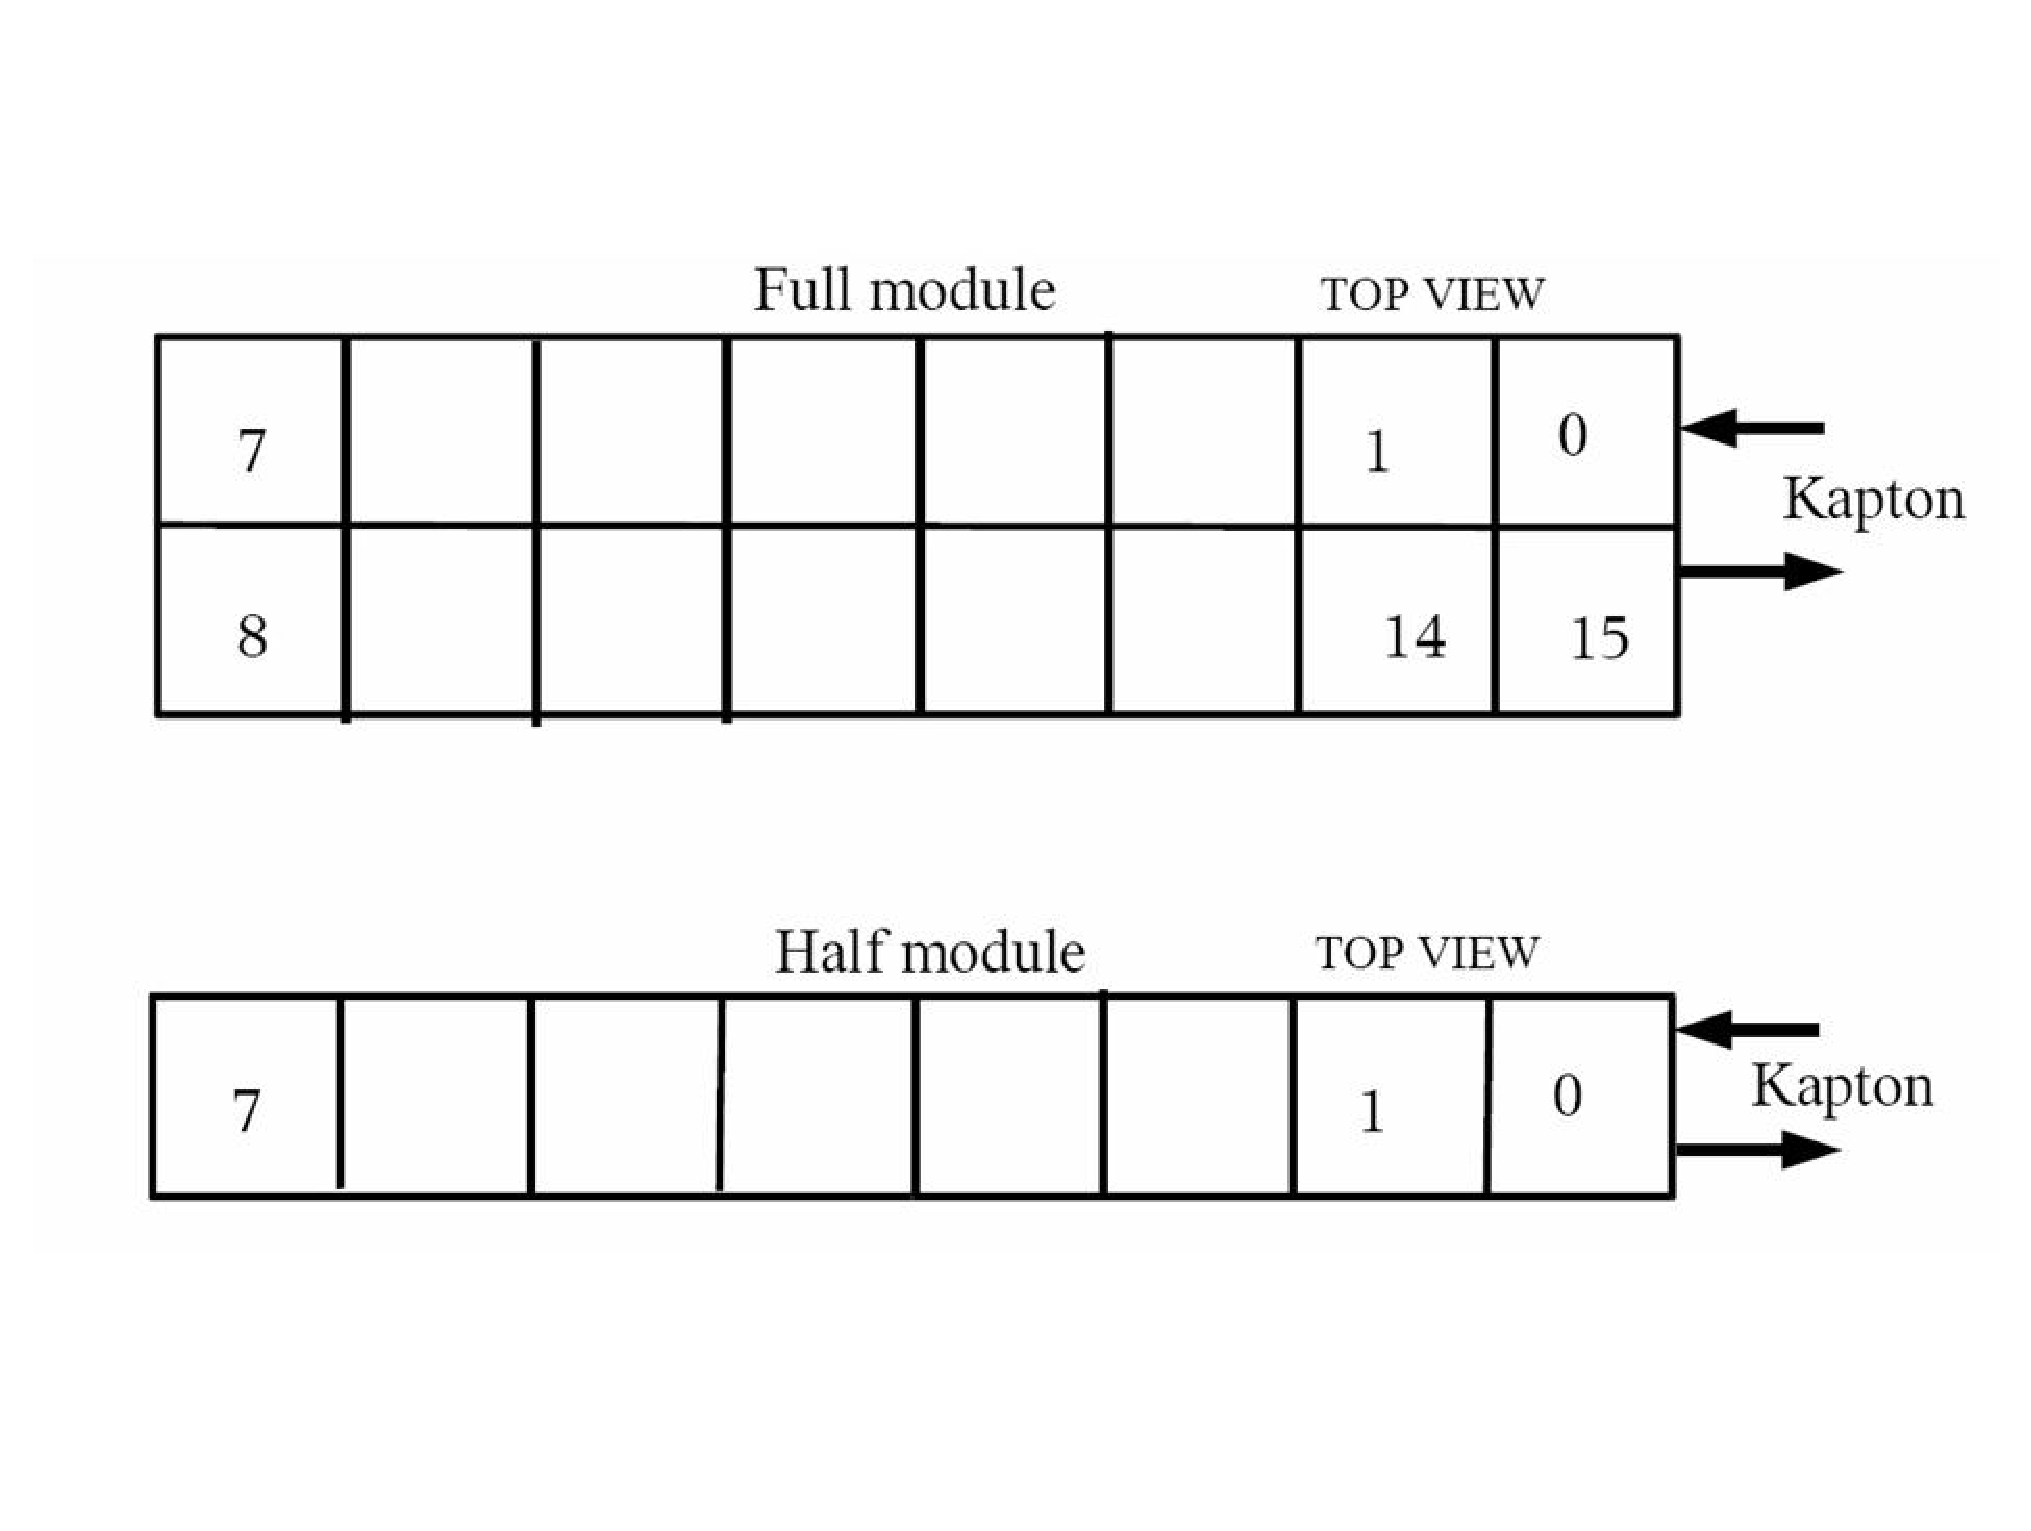
\includegraphics[width =0.6\textwidth]{barrel_roc_numbering.eps} 
    \caption{Numbering scheme for ROCs for full modules (upper) and
half modules (lower).} 
    \label{figure:barrel_roc} 
  \end{center} 
\end{figure} 


\subsubsection{Pixel Number}

Within a readout chip, the pixel number is defined by its row and column 
address in the same manner as it is for the Forward Pixel detector.
Every pixel unit cell (PUC) on a ROC can be identified by a column number 
(COLi, i from 0 to 51) and a row number (ROWj, j from 0 to 79).

Thus, the names for individual pixels are of the form:
\begin{displaymath}
\mbox{BPix\_B(p,m)(I,O)\_SEC(1-8)\_LYR(1-3)\_LDR(1H,2F-(N-1)F,NH)
\_MOD(1-4)\_ROC(0-(7,15))\_COL(0-51)\_ROW(0-79).}
\end{displaymath}

The barrel pixel naming hierarchy from ladders to pixels is shown in
fig.~\ref{figure:barrel_hier2}.

\begin{figure}[hbtp] 
  \begin{center} 
        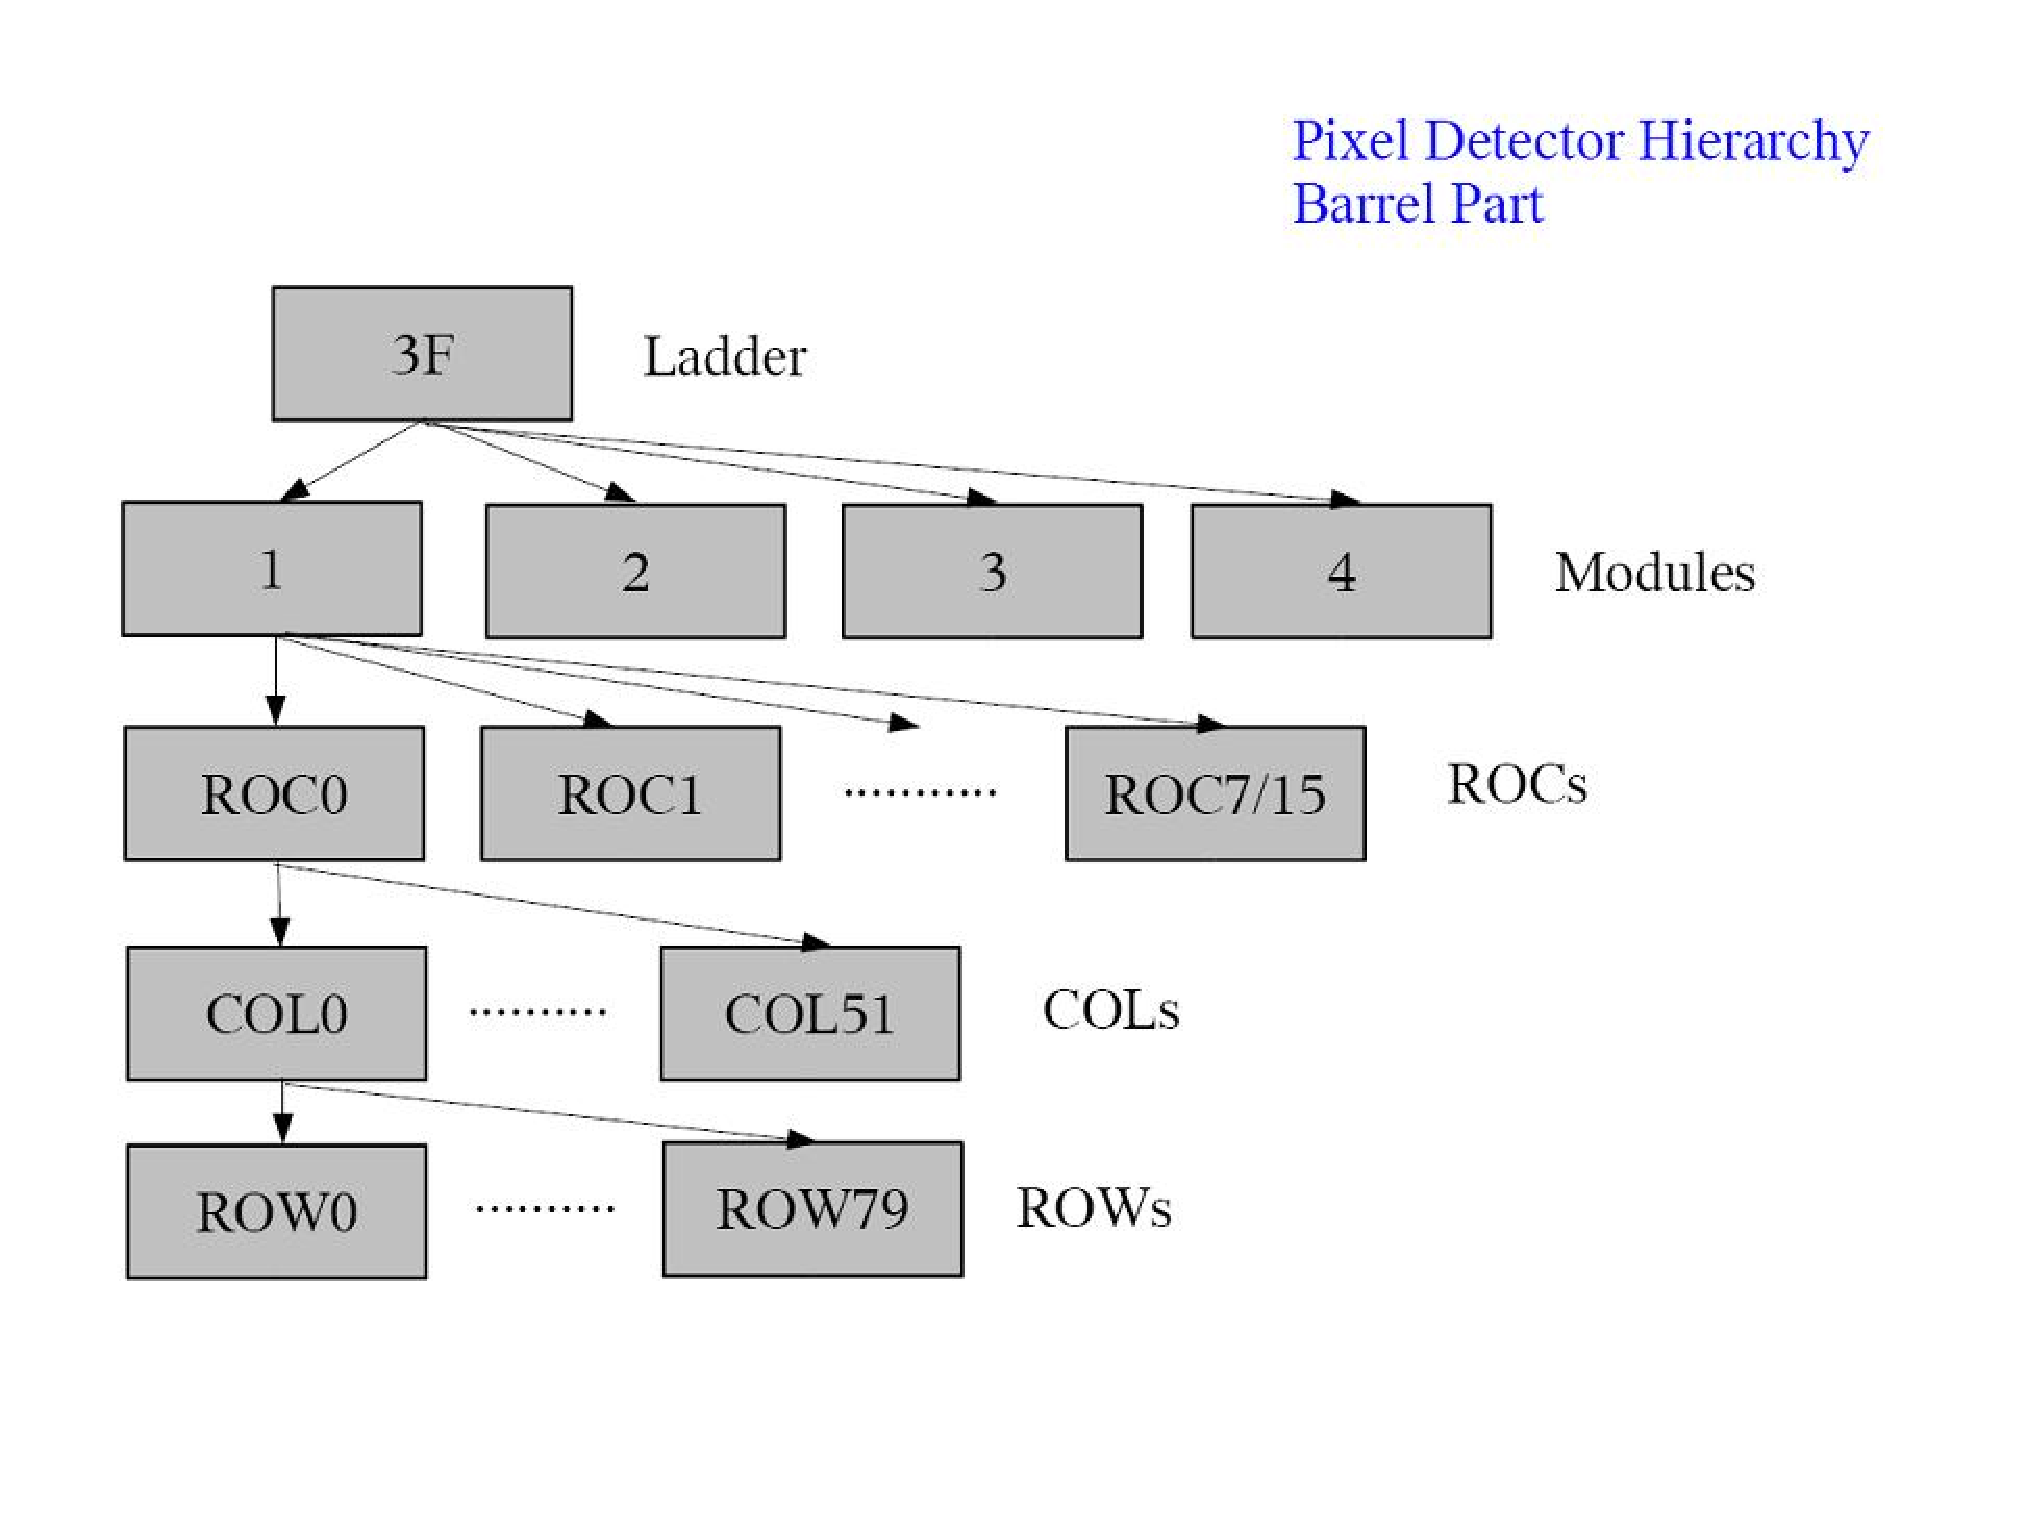
\includegraphics[width =0.8\textwidth]{barrel_hierarchy_2.eps} 
    \caption{Continuation of Barrel Pixel hierarchy from the ladder down to 
an indvidual pixel.} 
    \label{figure:barrel_hier2} 
  \end{center} 
\end{figure} 

%The names ``TRIM'' or ``MASK'' may be appended to this string with a hyphen, 
%to indicate either one of the two programmable registers of the PUC.

\subsubsection{The Supply Board and its Components}
 
The distribution of the incoming control signals, outgoing 
readout signals and the power is done in the barrel 
on the supply-board, shown in Fig.~\ref{figure:supply_board}.  
There is one supply-board, per detector sector, so there are 
all together 32 supply-boards which are placed on the 
front of the barrel supply-tube. 
The supply boards are named after the sector they are in:
$\mbox{BPix\_B(p,m)(I,O)\_SB(1-8).}$
 
Each supply board has a AOH-motherboard which includes 
six 6-channel AOHs (with the ALT chips). Four AOHs
(AOH 1-4 on fig.) are for layers 1 and 2 and 
two AOHs (AOH 5-6) are for layer 3. 
Presently we still do not know the exact AOH-fiber to 
module connection map since the endflage prints are still 
under development.
An AOH of a shell is named as:
$\mbox{BPix\_B(p,m)(I,O)\_SB1-8)\_AOH(1-6).}$

The second component of the supply board is the 
DOH-motherboard which has 2 control channels.
One control channel (called 1 and 2) is for modules 
in layer 1 and 2, the 2nd channel (called 3) is 
for modules in layer 3. Each channel has a DOH, PLL,
Delay25 (DL) and a GateKeeper (GK). The components 
which have I2C registers are programmed from the CCU-card
which is external to the supply-board.
The two control networks are named after the sector and 
the layer that they service.

   
The power distribution is similar, layers 1 and 2 are powered 
by two channels (Vanalog and Vdigital) and layer 3 by 
another two channels. Therefore there are 4 independent 
power channels per sector. The bias voltage has also 
4 channels, one for layer 1, one for layer 2 and two
for layer 3. The power and bias channels are named 
after the detector ladders which they service.

(Should we include the I2C addresses of all devices on 
the supply board?)

\begin{figure}[hbtp] 
  \begin{center} 
        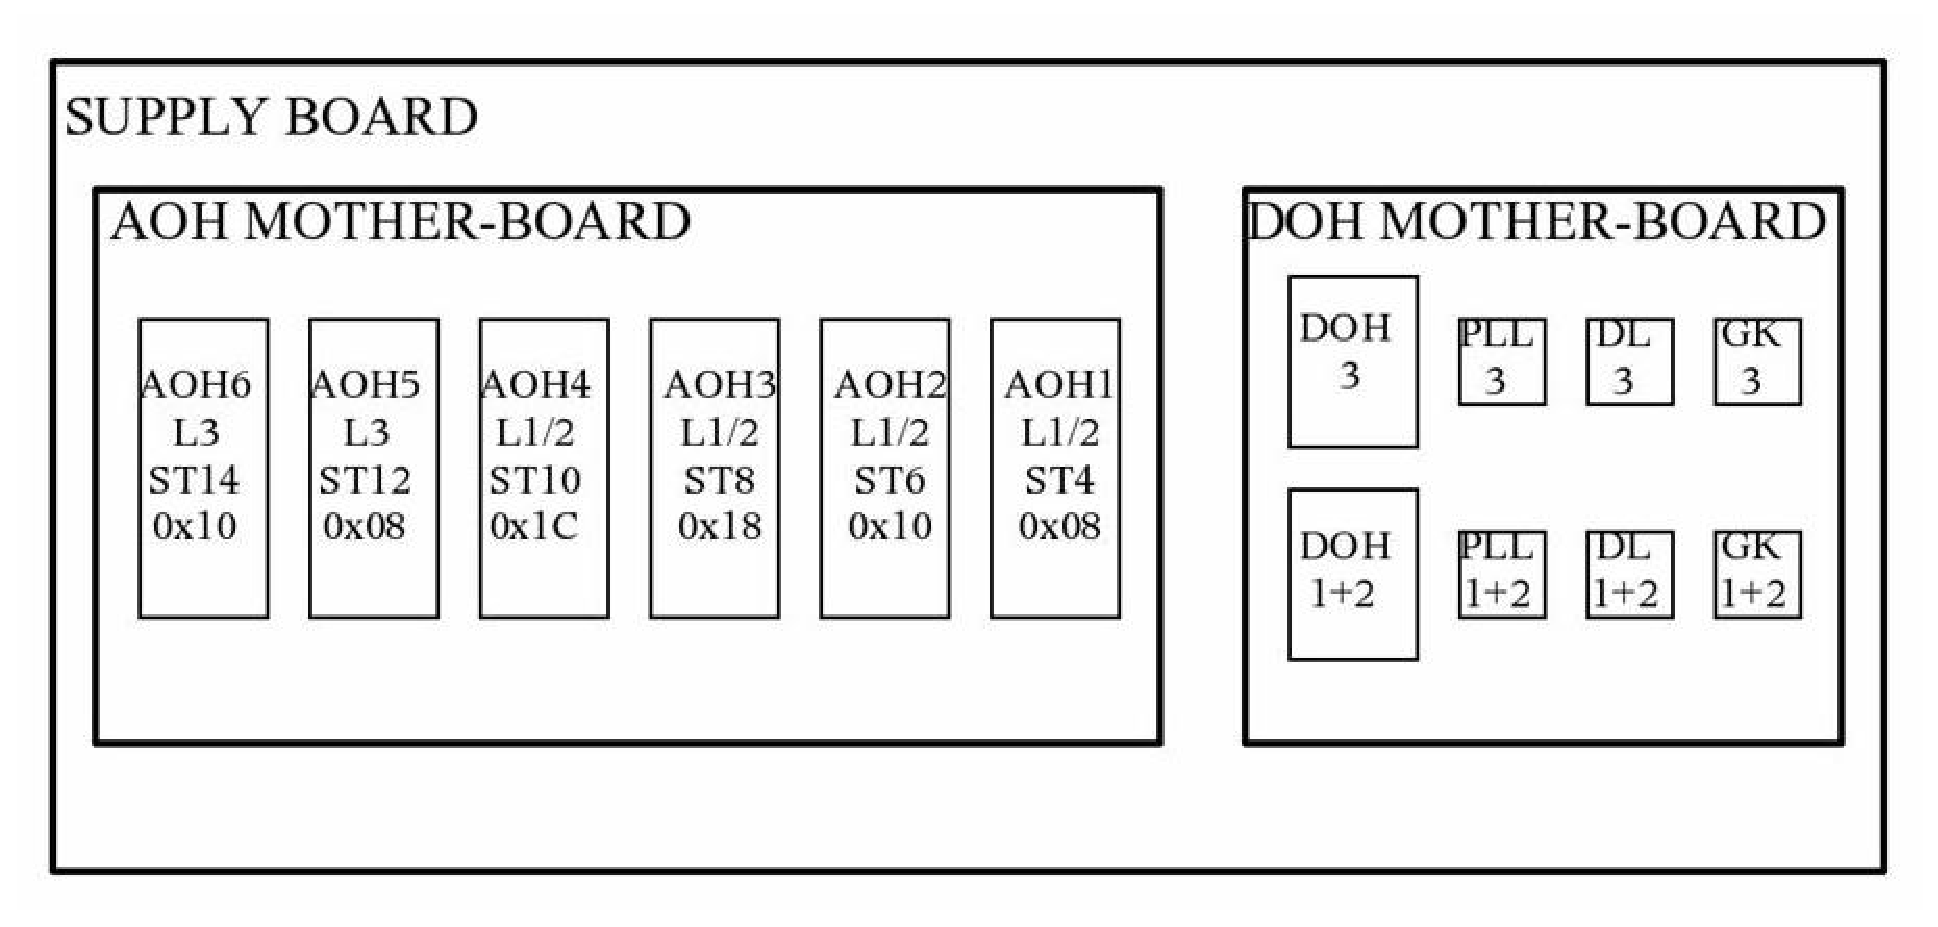
\includegraphics[width =0.6\textwidth]{supply_board.eps} 
    \caption{Layout of Barrel Pixel Supply Board} 
    \label{figure:supply_board} 
  \end{center} 
\end{figure} 

\subsubsection{CCU Board and its Components}

A number of devices have to be programmed using the 
standard CMS FEC-CCU system. For this purpose the barrel
has 4 CCU-boards placed in the back of the supply tube.
One CCU-board services one barrel shell (e.g. BpI),
therefore CCU-boards are identified by the shell
name.  
One CCU-board has a token ring with 8 active CCUs 
(numbered 1-8), 1 dummy CCU (numbered 9) for redundancy 
reasons and 2 DOHs. 
Each of the 8 CCUs provides I$^{2}$C signals to all devices in 
one sector.
Two output ports are used, one (Port 1) for Layer 1 and 2
and the second one (Port 3) for layer 3. In addition 
CCU-1 and CCU-2 use a 3rd port (Port-0) to program
the two local DOHs. 
The CCUs (1-8) can be called by the name of the sector 
they service. 
%The ninth CCU (CCU-9) is a dummy used only 
%for redundancy reasons. 
The DOHs are labeled 
according to the standard mFEC channel names A and B.
DOH-A is programmed by CCU-1 and DOH-B by CCU-2.   

\subsubsection{The Control Board}

Each half-shell is connected to two sensor cables for temperature and 
humidity readout (DCS). This cable will be attached
to the Control board where the wires are routed to
the temperature and humidity sensors. 

%There will 
%be 19 temperature sensors and 1 humidity sensor per
%shell. Each sector/slot will have 2 temperature sensors.
%The remaining 3 temperature sensors and the humidity
%sensor will be located in the "central" empty slot.
%
%(Sorry, for the moment I cannot give more details.
%While the number of sensors is fixed the exact location
%has not been yet decided.)


\section{Control Room Electronics}

The electronics that controls the pixel detector resides in the underground
control room called US5. 
There are two basic subsystems:
\begin{itemize}
\item A VME-based system, controlled by both local and remote computers.
The VME based system transmits control information to the on-detector 
electronics via optical fibers, using the two protocols I$^{2}$C and its faster variant PSI$^{2}$C,
and readouts the event data from the ROCs and transmits them 
to the Builder Units and HLT filter farms.
This system is controlled by the XDAQ software.
\item A commercial Slow Control System that manages the high and low voltages
in the system and monitors temperature, humidity and other characteristics
of the physical environment.
\end{itemize}

The hardware in these two systems is identical for the Barrel and
Forward Pixel detector.


\subsection{VME/XDAQ Components}

The relevant components are the VME crates and boards 
and the physically-connected rack-mounted Linux PCs. 
The naming convention for the rack and crate has already been defined by CMS.
A rack number followed by a crate location number is used to identify the VME 
crates. The location of a board within the VME crate is identified by the 
number of the slot in which the board is plugged into.
In addition, the name of the module includes an identifier, the ``type'', which describes its function.
For the Pixel detector, we have only a few types of modules.
Specifically, the modules used to control the Pixel detector electronics 
and readout the event data from the ROCs are PxlFED, PxlFEC, TrkFEC 
(a.k.a. the ``Tracker FEC''), TTC, LTC and CTRL.

\begin{itemize}
\item FED is an abbreviation for ``Front End Driver'' and denotes the module that
delivers the collision data to the data acquisition system. The prefix
``Pxl'' is used to differentiate this module from Front End Drivers for
other devices such as the Microstrip Tracker which is quite different; 
\item FEC stands for 
``Front End Controller'' and provides control and monitoring through VME of
all the chips on the detector. Two different types of FECs are used in controlling the Pixel detector:
\begin{itemize}
\item The PxlFEC controls the TBM and the Pixel 
Readout chips using the special pixel super-fast PSI$^{2}$C protocol; and 
\item The TrkFEC talks to a few specific chips on the Port Card
using the same standard I$^{2}$C protocol as the Microstrip Tracker.
\end{itemize}
\item TTC denotes the Timing and Trigger Control Module;
\item LTC is the Local Trigger Control;
\item CTRL is the VME controller; and 
\end{itemize}

The names for a VME board are of the form:
$\mbox{RackID\_CrateID\_s(slot ID)-(xxxx),}$
where (xxxx) is its module type 
(i.e. either PxlFED, PxlFEC, TrkFEC, TTC, LTC or CTRL). 

Following the pre-determined naming convention for VME crates, 
Table~\ref{table:us5:vme} lists the VME boards related to
the Forward Pixel detector. 

  \begin{table}[htb]
    \caption{List of electronics components for Forward Pixel detector at US5.
These are all in the same relay rack. The Linux PCs are in a different relay rack 
and are not included in the table.}
    \label{table:us5:vme}
    \begin{center}
      \begin{tabular}{l|lll} \hline
Crate ID&         S1G01e&                 S1G03e&                 S1E02p\\\hline
CAEN controller& S1G01e\_S01-CTRL&  S1G03e\_S01-CTRL&  S1E02p\_S01-CTRL\\
VME boards&         S1G01e\_S05-PxlFEC&  S1G03e\_S06-PxlFED&  S1E02p\_S02-LTC\\
&                 S1G01e\_S06-PxlFEC&  S1G03e\_S07-PxlFED&  S1E02p\_S08-TTCci\\
&                 &                  S1G03e\_S08-PxlFED&  S1E02p\_S09-TTCex\\
&                 &                  S1G03e\_S09-PxlFED&  \\
&                 &                  S1G03e\_S10-PxlFED&  \\
&                 &                  S1G03e\_S11-PxlFED&  \\
&                 &                  S1G03e\_S12-PxlFED&  \\
&                 S1G01e\_S06\_TrkFEC&  S1G03e\_S13-PxlFED&  \\ \hline
      \end{tabular}
    \end{center}
  \end{table}

In each one of the VME modules (PxlFEC, TrkFEC, and PxlFED), there are 
several optical input/output channels. These are labeled from top to 
bottom of the board as Ch1 to Ch36 for PxlFED, Ch1 to Ch8 for 
TrkFEC, and Ch1 to Ch16 for PxlFEC modules. 
Here each ``channel'' physically includes 
one or several optical fibres.  

%These channels of the FECs or FEDs represent
%physical connections (optical fibers). 
As an example, the channels of a PxlFEC module (S1G01e\_S06-PxlFEC), 
plugged into slot 6 of a VME crate, are named as:
$\mbox{S1G01e\_S06-PxlFEC\_Ch(1-16);}$
the channels of a TrkFEC module (S1G01e\_S13-TrkFEC),
plugged into slot 13 of a VME crate, are named as:
$\mbox{S1G01e\_S13-TrkFEC\_Ch(1-8); and}$
the channels for a PxlFED module (S1G03e\_S08-PxlFED),
plugged into slot 8 of a VME crate, are named as:
$\mbox{S1G03e\_S08-PxlFED\_Ch(1-36).}$

The PxlFECs and TrkFECs transmit PSI$^{2}$C and standard I$^{2}$C messages 
to the chips on the detector and receive data back from them. Each channel of a FEC controls
several devices attached to a single Port Card or Token Bit Manager (TBM). 
Similarly, each channel 
of a FED receives data from one TBM. These associations are made through a
database. This will be discussed below.

%A few concerns:
%\begin{itemize}
%\item \textcolor{red}{One thing is not mentioned here is the location and 
%naming of the tree optical coupler.}
%\end{itemize}

\subsubsection{TrackerFEC Control Network Assignments}

Devices on the Port Cards are conrtolled by the Tracker FEC, which is a VME 
module. There is only one Tracker FEC for the whole FPIX detector, named 
$\mbox{FPix\_TrkFEC.}$

The Tracker FEC has 4 subunits called MFEC(1-4), each of  which 
controls all the slow I$^{2}$C devices of one  
half-cylinder. Each MFEC communicates with 4 CCU controllers which
control one sector ($\phi$-slice) of this half-cylinder. The CCU controllers are named 
CCUS(1-4). Each CCUS controls another 3 CCU controllers which talk to 
individual half-disks. The latter are called CCUD(1-3). 

\begin{displaymath}
\mbox{FPix\_TrkFEC\_MFEC(1-4)\_CCUS(1-4)\_CCUD(1-(2,3)).}
\end{displaymath}

This name may be associated to the control of specific groups of readout
chips through the one-to-one mapping of this name to a unique 
Port Card/Adapter Board combination.

\begin{displaymath}
\mbox{FPix\_B(p,m)(I,O)\_D(1-3)\_PRT(1-4).}
\end{displaymath}

The address is extended for individual
devices and registers as follows:

\begin{displaymath}
\mbox{FPix\_TrkFEC\_MFEC(1-4)\_CCUS(1-4)\_CCUD(1-(2,3))\_devname-regname.}
\end{displaymath}

To make the proper associations, the following information must be available in 
%(presumed) small tables of 
the Configuration Database:
\begin{itemize}
\item the VME address of the Tracker FEC
\item the correspondance of the four half-cylinders - BpI, BpO, BmI, and BmO
with the four MFECs, MFEC(1-4).
\item the correspondence of the four CCUSs with the four sectors of the 
half-cylinders.
\item the correspondence of the 3 CCUDs with the three disks
\item the I$^{2}$C channel address on the CCUD
of each chip mounted on the Port Card (AOH, PLL, DEL, DOH, DCU).
\end{itemize}

\begin{table}[htb]
    \caption{FEC link assignments for Port Cards, Blades and Panels for half-cylinders BpI and BpO of the Forward Pixel detector. 
The assignments
all refer to a single PixelFEC.}
    \label{table:trkFEC_Bp}
    \begin{center}
      \begin{tabular}{l|c|c|ccc|ccc|ccc} \hline
Half & mfec &  CCU & \multicolumn{3}{|c|}{Disk 1} & 
\multicolumn{3}{|c}{Disk 2}  &    \multicolumn{3}{|c|}{Disk 3} \\ 
Cyl     & id & No.& prt(i$^{2}$c) & bld & pnl &  prt(i$^{2}$c) & bld & pnl &  
prt(i$^{2}$c) & bld & pnl \\  \hline
BpI & 1 & 1 & 1(1) & 1 & 1 & 1(2)  & 1 & 1 & 1(3)&   1 & 1  \\ \hline
      \end{tabular}
    \end{center}
  \end{table}

\subsubsection{PixelFEC Control Network Assignments}

The PixelFEC is a modified version of the FEC that is designed to 
facilitate control of the pixel readout chips. Each PixelFEC has
8 MFECS and each MFEC has two ``MFEC links.'' We will refer to the 
pixel FEC by number, PixFEC(1-4) and the MFEC links as MFEC(1-16).

Each MFEC link controls the ROCs on one disk of a $\phi$-slice or alternatively
the ROCs on one Adapter Board/Port Card. The MFEC link uses a TBM 
``hub address'' to control the ROCs on each panel.

The total number of PixelFECs is equal to the number of Adapter Boards (Port
Cards). Each half-disk has 4 Adapter Boards and for a 3-disk system,
a half-cylinder has 12 Adapter Boards/Port Cards. We are planning to
use one PixelFEC for each half-cylinder (4 PixelFECs in total; see above).
This means that only 8(12) MFEC links out of 16 in the PixelFEC will be used
in a 2(3) disk system.


\begin{table}[htb]
    \caption{MFEC link assignments for Port Cards, Blades, Panels and 
corresponding TBM Hub assignments for half-cylinders BpI and BpO. 
These assignments
all refer to a single PixelFEC. ``hub'' refers to TBM Hub.}
    \label{table:pixelFEC_Bp}
    \begin{center}
      \begin{tabular}{l|l|cccc|l|cccc|l|cccc} \hline
Half & mfec &  \multicolumn{4}{|c|}{Disk 1} & mfec  & 
\multicolumn{4}{|c}{Disk 2}  &   
mfec  & \multicolumn{4}{|c|}{Disk 3} \\ 
Cyl     & link & prt & bld & pnl & hub & link & prt & bld & pnl & hub &
link & prt & bld & pnl & hub \\  \hline
BpI & 1 & 1 & 1 & 1 & 14 & 2  & 1 & 1 & 1& 14 & 3 & 1 & 1 & 1& 14 \\ \hline
    &   &   & 1 & 2 & 6  &    &   & 1 & 2&  6 &   &   & 1 & 2&  6 \\ \hline
    &   &   & 2 & 1 & 13 &    &   & 2 & 1& 13 &   &   & 2 & 1& 13 \\ \hline
    &   &   & 2 & 2 & 5  &    &   & 2 & 2& 5  &   &   & 2 & 2& 5 \\ \hline
    &   &   & 3 & 1 & 12 &    &   & 3 & 1& 12 &   &   & 3 & 1& 12 \\ \hline
    &   &   & 3 & 2 & 4  &    &   & 3 & 2& 4  &   &   & 3 & 2& 4 \\ \hline
    & 4 & 2 & 4 & 1 & 14 & 5  & 2 & 4 & 1& 14 & 6 & 2 & 4 & 1& 14 \\ \hline
    &   &   & 4 & 2 &  6 &    &   & 4 & 2&  6 &   &   & 4 & 2& 6 \\ \hline
    &   &   & 5 & 1 & 13 &    &   & 5 & 1& 13 &   &   & 5 & 1& 13 \\ \hline
    &   &   & 5 & 2 &  5 &    &   & 5 & 2&  5 &   &   & 5 & 2&  5 \\ \hline
    &   &   & 6 & 1 & 12 &    &   & 6 & 1& 12 &   &   & 6 & 1& 12 \\ \hline
    &   &   & 6 & 2 &  4 &    &   & 6 & 2&  4 &   &   & 6 & 2&  4 \\ \hline
    & 7 & 3 & 7 & 1 & 14 & 8  & 3 & 7 & 1& 14 & 9 & 3 & 7 & 1& 14 \\ \hline
    &   &   & 7 & 2 &  6 &    &   & 7 & 2&  6 &   &   & 7 & 2&  6 \\ \hline
    &   &   & 8 & 1 & 13 &    &   & 8 & 1& 13 &   &   & 8 & 1& 13 \\ \hline
    &   &   & 8 & 2 &  5 &    &   & 8 & 2&  5 &   &   & 8 & 2&  5 \\ \hline
    &   &   & 9 & 1 & 12 &    &   & 9 & 1& 12 &   &   & 9 & 1& 12 \\ \hline
    &   &   & 9 & 2 &  4 &    &   & 9 & 2&  4 &   &   & 9 & 2&  4 \\ \hline
    & 10& 4 & 10 & 1 & 14 & 11& 4 & 10& 1& 14 & 12& 4 & 10 & 1& 14 \\ \hline
    &   &   & 10 & 2 &  6 &    &   & 10 & 2&  6 &   &   & 10 & 2&  6 \\ \hline
    &   &   & 11 & 1 & 13 &    &   & 11 & 1& 13 &   &   & 11 & 1& 13 \\ \hline
    &   &   & 11 & 2 &  5 &    &   & 11 & 2&  5 &   &   & 11 & 2&  5 \\ \hline
    &   &   & 12 & 1 & 12 &    &   & 12 & 1& 12 &   &   & 12 & 1& 12 \\ \hline
    &   &   & 12 & 2 &  4 &    &   & 12 & 2&  4 &   &   & 12 & 2&  4 \\ \hline
\hline
BpO & 1 & 1 & 1 & 1 & 12 & 2  & 1 & 1 & 1& 12 & 3 & 1 & 1 & 1& 12 \\ \hline
    &   &   & 1 & 2 &  4 &    &   & 1 & 2&  4 &   &   & 1 & 2&  4 \\ \hline
    &   &   & 2 & 1 & 13 &    &   & 2 & 1& 13 &   &   & 2 & 1& 13 \\ \hline
    &   &   & 2 & 2 &  5 &    &   & 2 & 2&  5 &   &   & 2 & 2&  5 \\ \hline
    &   &   & 3 & 1 & 14 &    &   & 3 & 1& 14 &   &   & 3 & 1& 14 \\ \hline
    &   &   & 3 & 2 &  6 &    &   & 3 & 2&  6 &   &   & 3 & 2&  6 \\ \hline
    & 4 & 2 & 4 & 1 & 12 & 5  & 2 & 4 & 1& 12 & 6 & 2 & 4 & 1& 12 \\ \hline
    &   &   & 4 & 2 &  4 &    &   & 4 & 2&  4 &   &   & 4 & 2&  4 \\ \hline
    &   &   & 5 & 1 & 13 &    &   & 5 & 1& 13 &   &   & 5 & 1& 13 \\ \hline
    &   &   & 5 & 2 &  5 &    &   & 5 & 2&  5 &   &   & 5 & 2&  5 \\ \hline
    &   &   & 6 & 1 & 14 &    &   & 6 & 1& 14 &   &   & 6 & 1& 14 \\ \hline
    &   &   & 6 & 2 &  6 &    &   & 6 & 2&  6 &   &   & 6 & 2&  6 \\ \hline
    & 7 & 3 & 7 & 1 & 12 & 8  & 3 & 7 & 1& 12 & 9 & 3 & 7 & 1& 12 \\ \hline
    &   &   & 7 & 2 &  4 &    &   & 7 & 2&  4 &   &   & 7 & 2&  4 \\ \hline
    &   &   & 8 & 1 & 13 &    &   & 8 & 1& 13 &   &   & 8 & 1& 13 \\ \hline
    &   &   & 8 & 2 &  5 &    &   & 8 & 2&  5 &   &   & 8 & 2&  5 \\ \hline
    &   &   & 9 & 1 & 14 &    &   & 9 & 1& 14 &   &   & 9 & 1& 14 \\ \hline
    &   &   & 9 & 2 &  6 &    &   & 9 & 2&  6 &   &   & 9 & 2&  6 \\ \hline
    & 10& 4 & 10 & 1 & 12 & 11& 4 & 10& 1& 12 & 12& 4 & 10 & 1& 12 \\ \hline
    &   &   & 10 & 2 &  4 &    &  & 10& 2&  4 &   &   & 10 & 2&  4 \\ \hline
    &   &   & 11 & 1 & 13 &    &  & 11& 1& 13 &   &   & 11 & 1& 13 \\ \hline
    &   &   & 11 & 2 &  5 &    &  & 11& 2&  5 &   &   & 11 & 2&  5 \\ \hline
    &   &   & 12 & 1 & 14 &    &  & 12& 1& 14 &   &   & 12 & 1& 14 \\ \hline
    &   &   & 12 & 2 &  6 &    &  & 12& 2&  6 &   &   & 12 & 2&  6 \\ \hline
      \end{tabular}
    \end{center}
  \end{table}


\begin{table}[htb]
    \caption{MFEC link assignments for Port Cards, Blades, Panels and 
corresponding TBM Hub assignments  half-cylinders BmI and BmO. 
These assignments
all refer to a single PixelFEC. ``hub'' refers to TBM Hub.}
    \label{table:pixelFEC_Bm}
    \begin{center}
      \begin{tabular}{l|l|cccc|l|cccc|l|cccc} \hline
Half & mfec &  \multicolumn{4}{|c|}{Disk 1} & mfec  & 
\multicolumn{4}{|c}{Disk 2}  &   
mfec  & \multicolumn{4}{|c|}{Disk 3} \\ 
Cyl     & link & prt & bld & pnl & hub & link & prt & bld & pnl & hub &
link & prt & bld & pnl & hub \\  \hline
BmI & 1 & 1 & 1 & 1 & 12 & 2  & 1 & 1 & 1& 12 & 3 & 1 & 1 & 1& 12 \\ \hline
    &   &   & 1 & 2 & 4  &    &   & 1 & 2&  4 &   &   & 1 & 2&  4 \\ \hline
    &   &   & 2 & 1 & 13 &    &   & 2 & 1& 13 &   &   & 2 & 1& 13 \\ \hline
    &   &   & 2 & 2 & 5  &    &   & 2 & 2& 5  &   &   & 2 & 2& 5 \\ \hline
    &   &   & 3 & 1 & 14 &    &   & 3 & 1& 14 &   &   & 3 & 1& 14 \\ \hline
    &   &   & 3 & 2 & 6  &    &   & 3 & 2& 6  &   &   & 3 & 2& 6 \\ \hline
    & 4 & 2 & 4 & 1 & 12 & 5  & 2 & 4 & 1& 12 & 6 & 2 & 4 & 1& 12 \\ \hline
    &   &   & 4 & 2 &  4 &    &   & 4 & 2&  4 &   &   & 4 & 2& 4 \\ \hline
    &   &   & 5 & 1 & 13 &    &   & 5 & 1& 13 &   &   & 5 & 1& 13 \\ \hline
    &   &   & 5 & 2 &  5 &    &   & 5 & 2&  5 &   &   & 5 & 2&  5 \\ \hline
    &   &   & 6 & 1 & 14 &    &   & 6 & 1& 14 &   &   & 6 & 1& 14 \\ \hline
    &   &   & 6 & 2 &  6 &    &   & 6 & 2&  6 &   &   & 6 & 2&  6 \\ \hline
    & 7 & 3 & 7 & 1 & 12 & 8  & 3 & 7 & 1& 12 & 9 & 3 & 7 & 1& 12 \\ \hline
    &   &   & 7 & 2 &  4 &    &   & 7 & 2&  4 &   &   & 7 & 2&  4 \\ \hline
    &   &   & 8 & 1 & 13 &    &   & 8 & 1& 13 &   &   & 8 & 1& 13 \\ \hline
    &   &   & 8 & 2 &  5 &    &   & 8 & 2&  5 &   &   & 8 & 2&  5 \\ \hline
    &   &   & 9 & 1 & 14 &    &   & 9 & 1& 14 &   &   & 9 & 1& 14 \\ \hline
    &   &   & 9 & 2 &  6 &    &   & 9 & 2&  6 &   &   & 9 & 2&  6 \\ \hline
    & 10& 4 & 10 & 1 & 12 & 11& 4 & 10& 1& 12 & 12& 4 & 10 & 1& 12 \\ \hline
    &   &   & 10 & 2 &  4 &    &   & 10 & 2&  4 &   &   & 10 & 2&  4 \\ \hline
    &   &   & 11 & 1 & 13 &    &   & 11 & 1& 13 &   &   & 11 & 1& 13 \\ \hline
    &   &   & 11 & 2 &  5 &    &   & 11 & 2&  5 &   &   & 11 & 2&  5 \\ \hline
    &   &   & 12 & 1 & 14 &    &   & 12 & 1& 14 &   &   & 12 & 1& 14 \\ \hline
    &   &   & 12 & 2 &  6 &    &   & 12 & 2&  6 &   &   & 12 & 2&  6 \\ \hline
\hline
BmO & 1 & 1 & 1 & 1 & 14 & 2  & 1 & 1 & 1& 14 & 3 & 1 & 1 & 1& 14 \\ \hline
    &   &   & 1 & 2 &  6 &    &   & 1 & 2&  6 &   &   & 1 & 2&  6 \\ \hline
    &   &   & 2 & 1 & 13 &    &   & 2 & 1& 13 &   &   & 2 & 1& 13 \\ \hline
    &   &   & 2 & 2 &  5 &    &   & 2 & 2&  5 &   &   & 2 & 2&  5 \\ \hline
    &   &   & 3 & 1 & 12 &    &   & 3 & 1& 12 &   &   & 3 & 1& 12 \\ \hline
    &   &   & 3 & 2 &  4 &    &   & 3 & 2&  4 &   &   & 3 & 2&  4 \\ \hline
    & 4 & 2 & 4 & 1 & 14 & 5  & 2 & 4 & 1& 14 & 6 & 2 & 4 & 1& 14 \\ \hline
    &   &   & 4 & 2 &  6 &    &   & 4 & 2&  6 &   &   & 4 & 2&  6 \\ \hline
    &   &   & 5 & 1 & 13 &    &   & 5 & 1& 13 &   &   & 5 & 1& 13 \\ \hline
    &   &   & 5 & 2 &  5 &    &   & 5 & 2&  5 &   &   & 5 & 2&  5 \\ \hline
    &   &   & 6 & 1 & 12 &    &   & 6 & 1& 12 &   &   & 6 & 1& 12 \\ \hline
    &   &   & 6 & 2 &  4 &    &   & 6 & 2&  4 &   &   & 6 & 2&  4 \\ \hline
    & 7 & 3 & 7 & 1 & 14 & 8  & 3 & 7 & 1& 14 & 9 & 3 & 7 & 1& 14 \\ \hline
    &   &   & 7 & 2 &  6 &    &   & 7 & 2&  6 &   &   & 7 & 2&  6 \\ \hline
    &   &   & 8 & 1 & 13 &    &   & 8 & 1& 13 &   &   & 8 & 1& 13 \\ \hline
    &   &   & 8 & 2 &  5 &    &   & 8 & 2&  5 &   &   & 8 & 2&  5 \\ \hline
    &   &   & 9 & 1 & 12 &    &   & 9 & 1& 12 &   &   & 9 & 1& 12 \\ \hline
    &   &   & 9 & 2 &  4 &    &   & 9 & 2&  4 &   &   & 9 & 2&  4 \\ \hline
    & 10& 4 & 10 & 1 & 14 & 11& 4 & 10& 1& 14 & 12& 4 & 10 & 1& 14 \\ \hline
    &   &   & 10 & 2 &  6 &    &  & 10& 2&  6 &   &   & 10 & 2&  6 \\ \hline
    &   &   & 11 & 1 & 13 &    &  & 11& 1& 13 &   &   & 11 & 1& 13 \\ \hline
    &   &   & 11 & 2 &  5 &    &  & 11& 2&  5 &   &   & 11 & 2&  5 \\ \hline
    &   &   & 12 & 1 & 12 &    &  & 12& 1& 12 &   &   & 12 & 1& 12 \\ \hline
    &   &   & 12 & 2 &  4 &    &  & 12& 2&  4 &   &   & 12 & 2&  4 \\ \hline
      \end{tabular}
    \end{center}
  \end{table}


\subsection{DCS Electronics Components}

The Detector Control System (DCS), often referred to as 
the ``Slow Control and Monitoring System''
provides services to the Pixel Detectors that are not available through the
VME system, such as:
\begin{itemize}
\item Control and monitoring of the electrical power needed to operate all
 the electronics boards and read-out chips on the detector;
\item Control and monitoring of the the bias voltage needed to deplete the
pixel sensors;
\item Monitoring of the temperature at various points in the detector; and
\item Monitoring of the humidity in the gas volume surrounding the detector.
\end{itemize}

The placement of temperature and humidity sensors in the Forward and Barrel Pixel detectors is displayed in 
figures~\ref{figure:dcsSensorPlacementFPix} and~\ref{figure:dcsSensorPlacementBPix}, respectively.
The distribution of power for operation of the on-detector electronics and the depletion of the pixel sensors 
is illustrated in figure~\ref{figure:dcsPowerDistributionFPix} for the Forward and in figure~\ref{figure:dcsPowerDistributionBPix}
for the Barrel Pixel detector.
In total, 156 (76) RTD temperature sensors and 4 (4) HMX humidity sensors are mounted in the Forward (Barrel) Pixel detector.
The Forward (Barrel) Pixel detector is powered by 76 (164) low voltage and 64 (128) high voltage channels.

\begin{figure}[hbtp]
\setlength{\unitlength}{1mm}
\begin{center}
\begin{picture}(150,220)(0,0)
\put(5,115){\mbox{\epsfig{file = dcsSensorPlacement_v1.eps, width = 105mm,
                        bbllx=37, bblly=18, bburx=952, bbury=1236, angle=90}}}
\put(5,0){\mbox{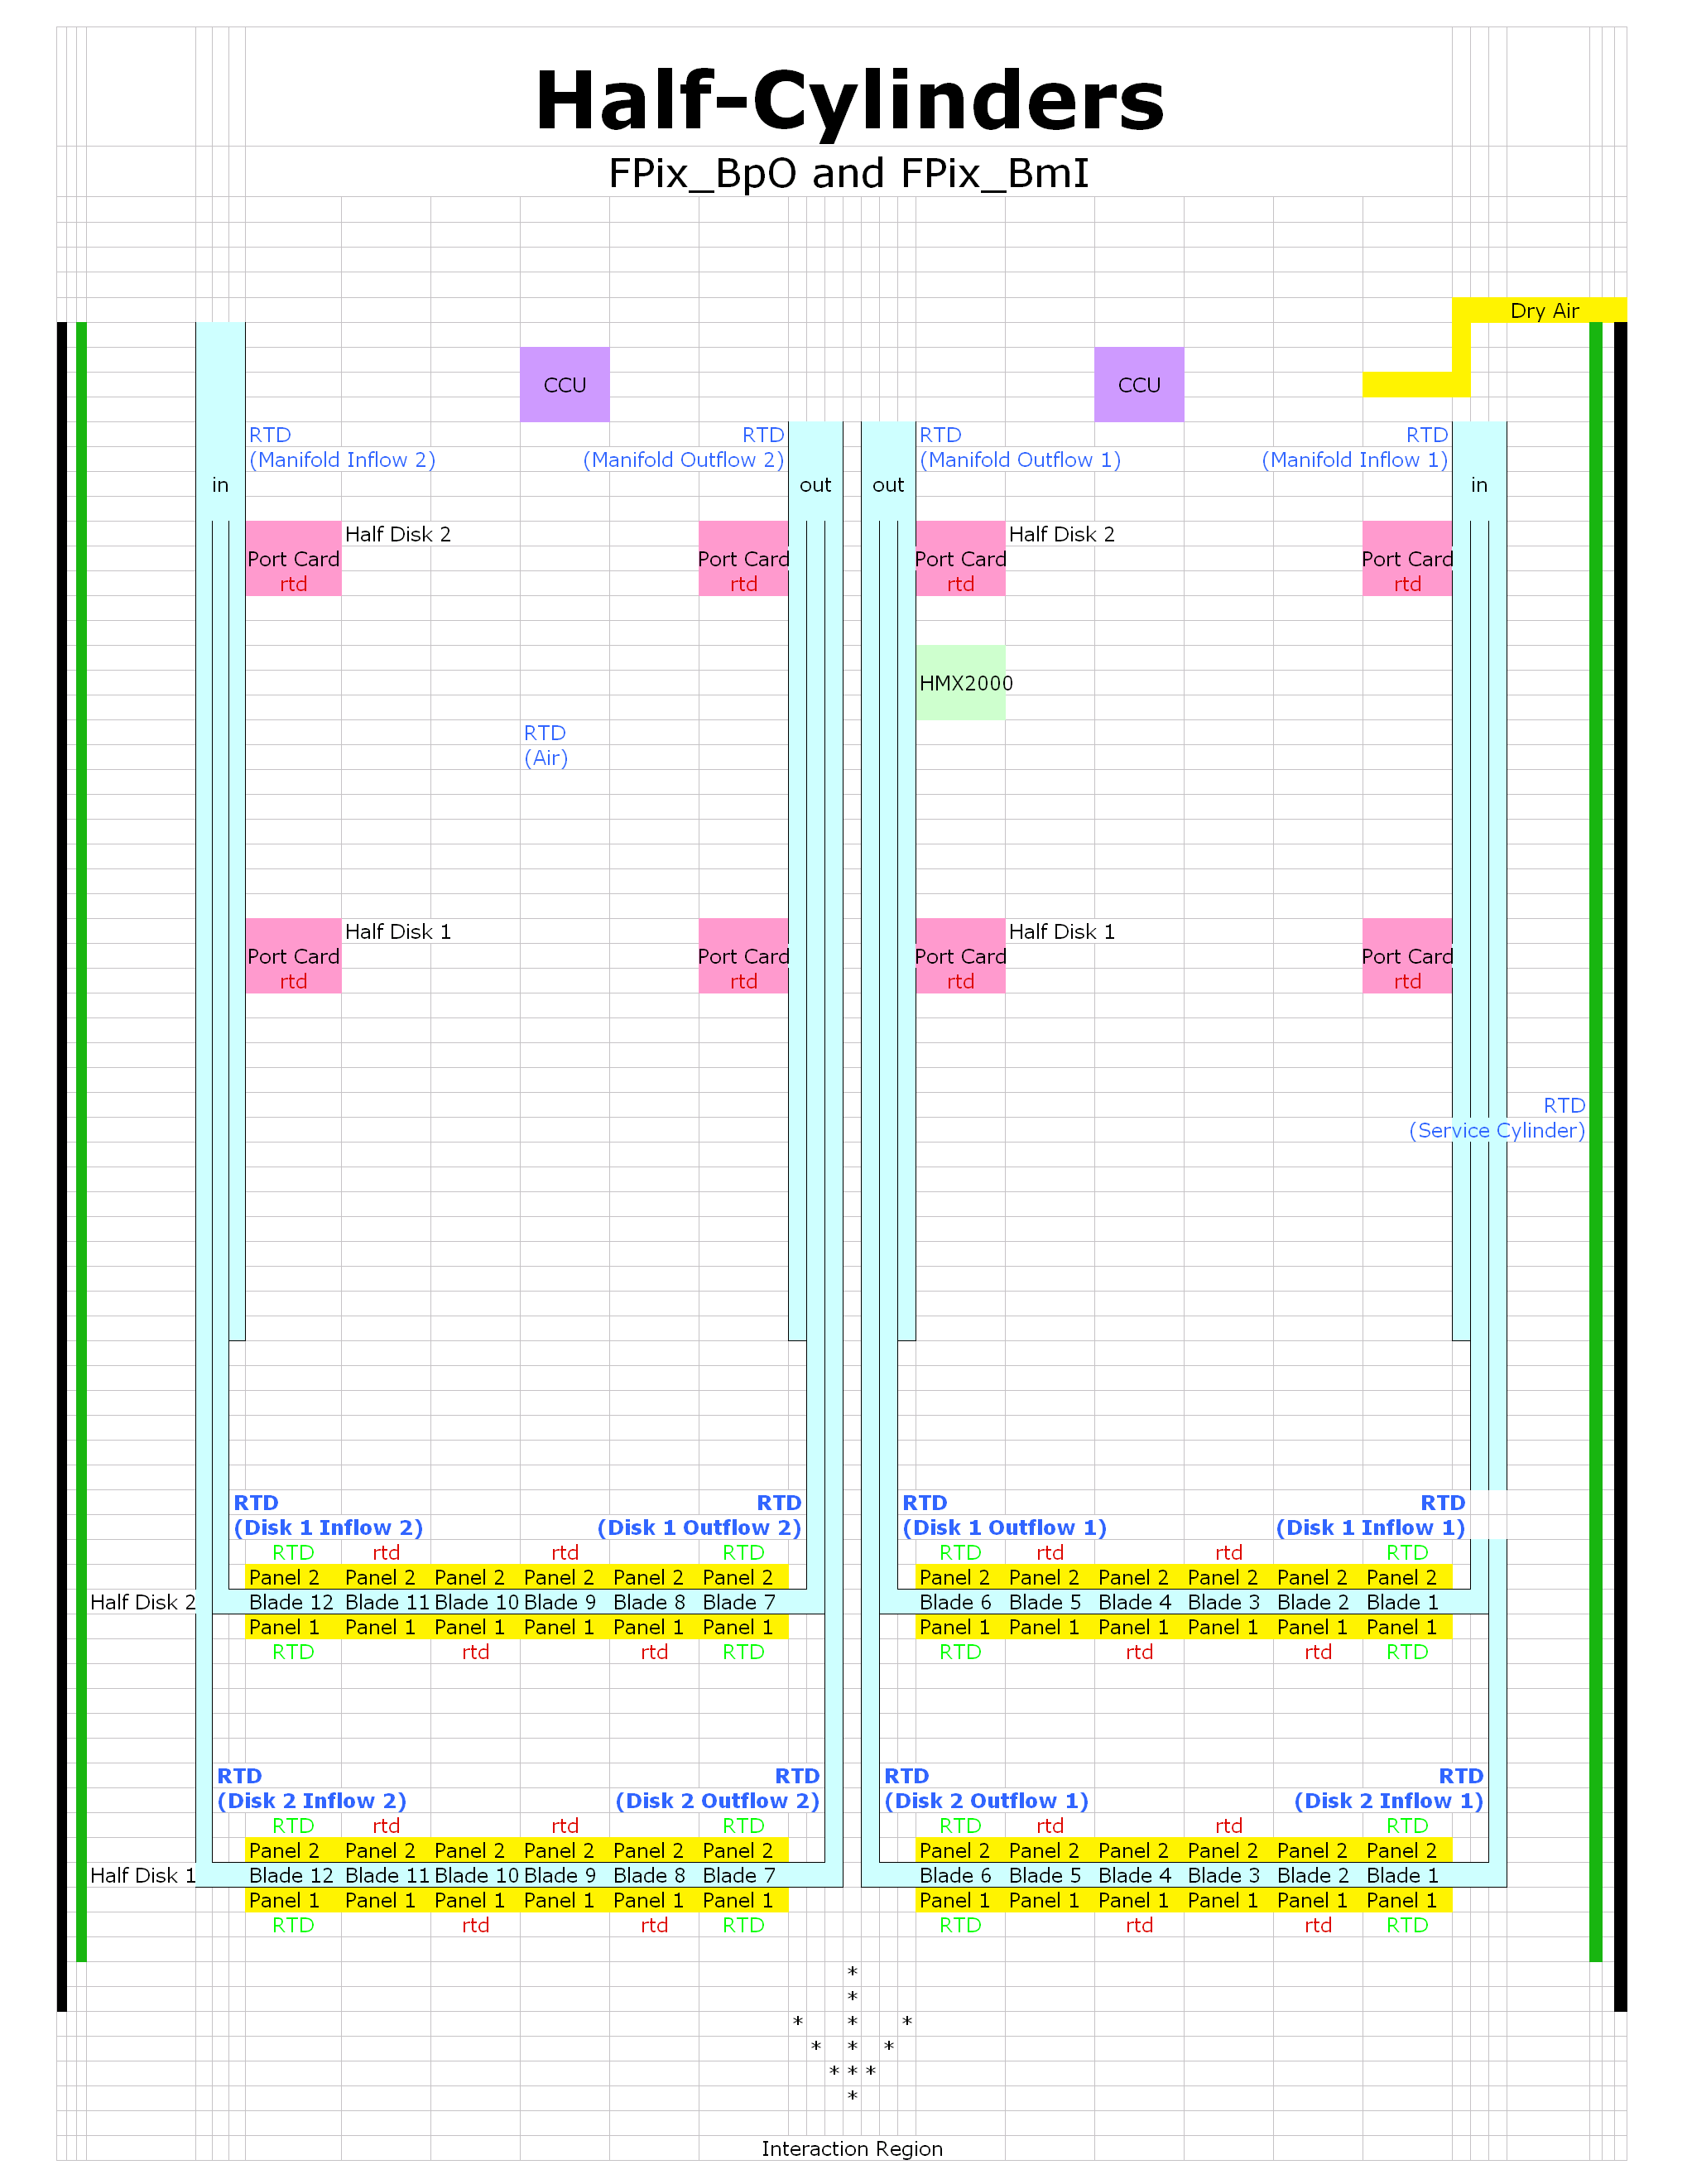
\epsfig{file = dcsSensorPlacement_v2.eps, width = 105mm,
                        bbllx=37, bblly=18, bburx=952, bbury=1236, angle=90}}}
\end{picture}
    \caption{Placement of temperature and humidity sensors in the half-cylinders of the Forward Pixel detector.
             Two mirror-symmetric layouts have been designed: one for the FPix\_BpO and FPix\_BmI half-cylinders (bottom/left side)
             and one for the FPix\_BpI and FPix\_BmO half-cylinders (top/right side).
             Depending on the kind of read-out, the temperature sensors are labeled as ``RTD'' (read-out via Siemens modules) and ``rtd'' (read-out via DCU).
             The humidity sensors are labeled as ``HMX''.}
    \label{figure:dcsSensorPlacementFPix}
  \end{center}
\end{figure}

\begin{figure}[hbtp]
  \begin{center}
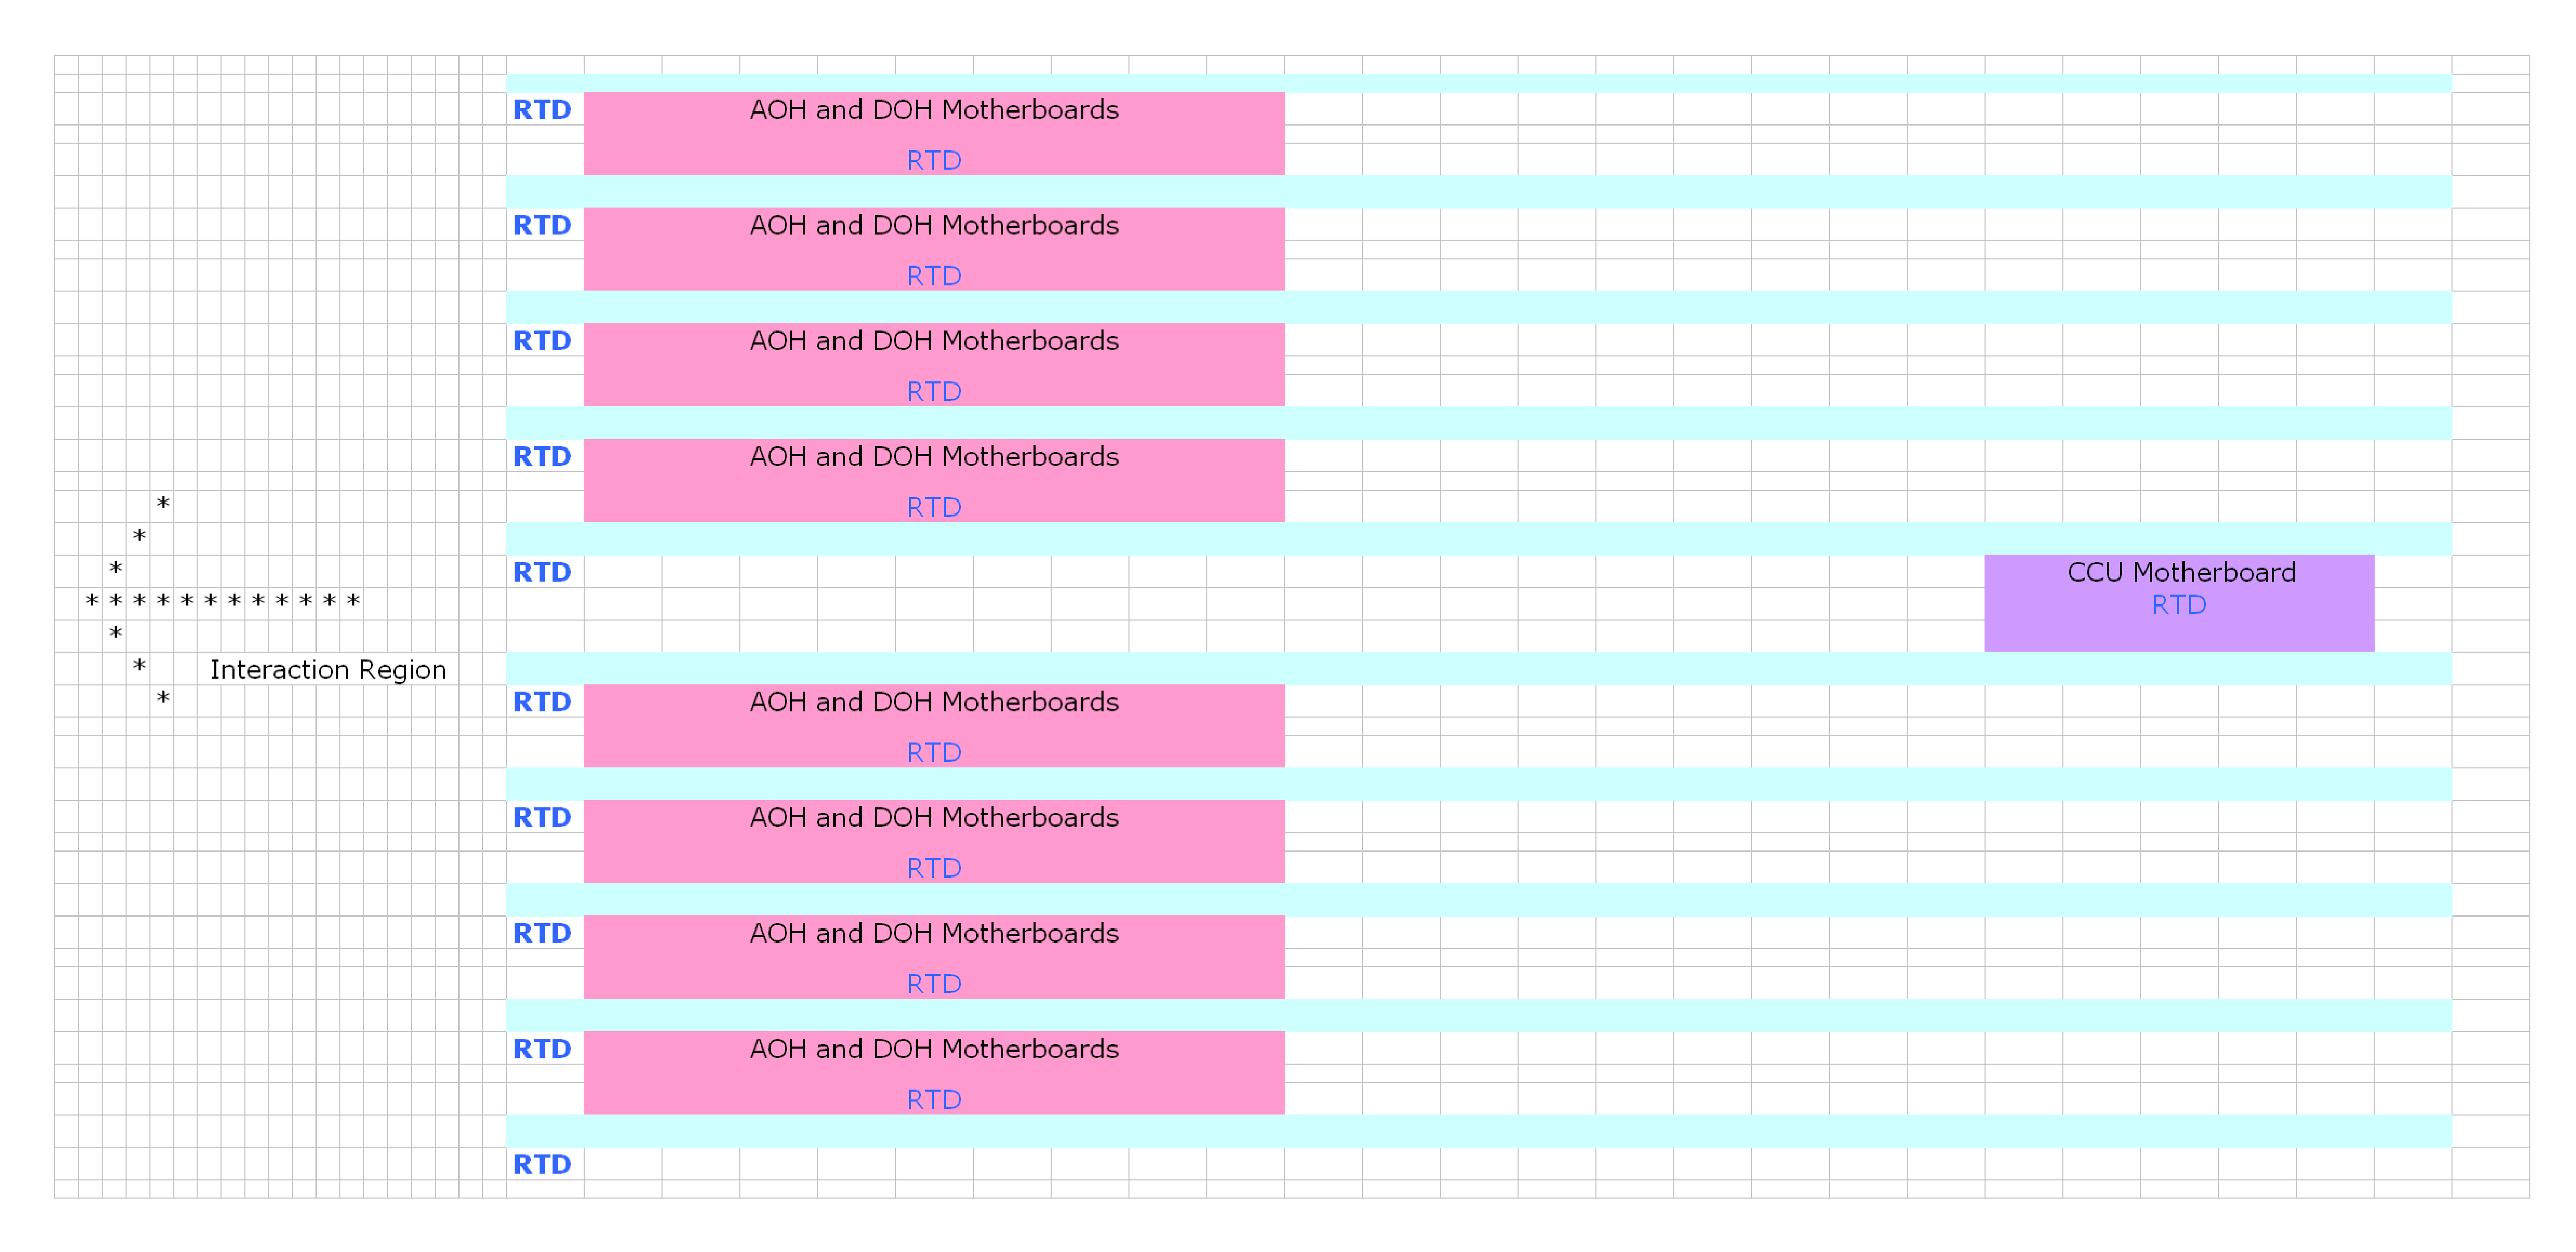
\epsfig{file = dcsSensorPlacementBPix.eps, height = 62mm,
        bbllx=100, bblly=149, bburx=2357, bbury=1213, clip=}
    \caption{Placement of temperature and humidity sensors in the shells of the Barrel Pixel detector.}
    \label{figure:dcsSensorPlacementBPix}
  \end{center}
\end{figure}

\begin{figure}[hbtp]
  \begin{center}
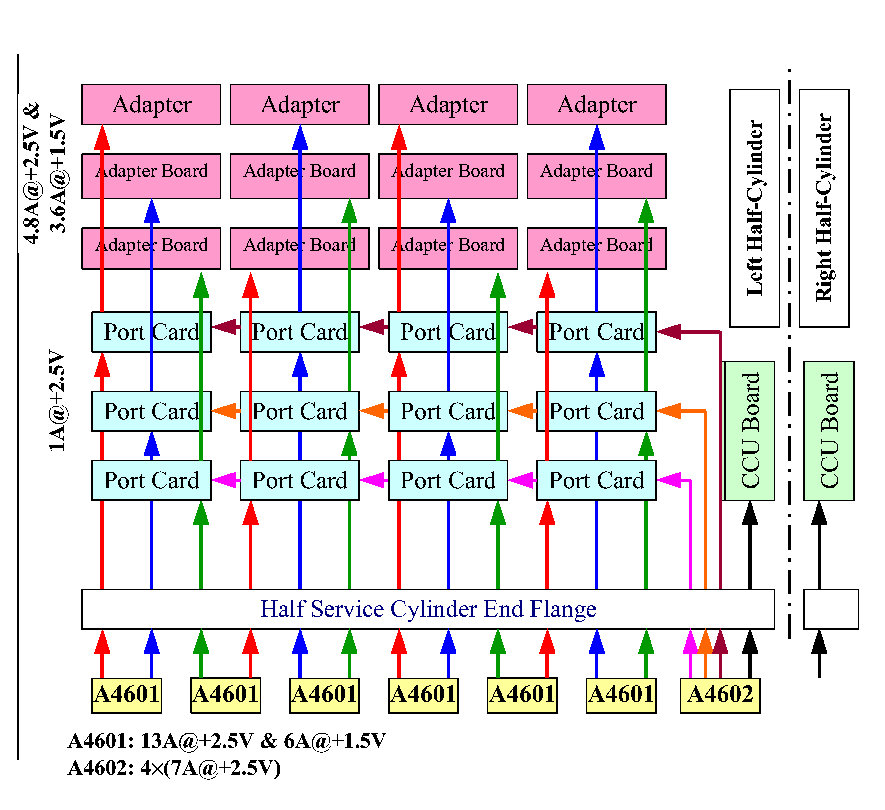
\epsfig{file = dcsPowerDistribution.eps, height = 85mm,
        bbllx=16, bblly=20, bburx=421, bbury=365, clip=}
    \caption{Distribution of power for detector operation and depletion of the sensors in the Forward Pixel detector
             (per half-cylinder for a three disk scenario).}
%             Each A4601 board consists of two power supply units (PSUs),
%             which each provide two low voltage channels, one at about 2.5V for the digital (signal processing) part of the read-out chips and
%             one at about 1.75V (not 1.5V as indicated in the figure) for the analog part (amplification and shaping of the charge signal) of the read-out chips
%             plus two high voltage channels that can be independently set between 0-600V (having two high voltage channels instead of one allows the plaquettes
%             that are closer to the beam-pipe and hence receive more radiation damage to be operated at a higher bias voltage).
%             The A4602 board also consists of two PSUs each.
%             The PSUs of the A4602 type boards provide four low voltages of 2.5V for the operation of electronics on the Port Cards and CCU motherboards.}
    \label{figure:dcsPowerDistributionFPix}
  \end{center}
\end{figure}

\begin{figure}[hbtp]
\setlength{\unitlength}{1mm}
  \begin{center}
\begin{picture}(150,66)(0,0)
\put(-8,66){\mbox{\large \bf Barrel detector:}}
\put(-8,62){\mbox{\large \bf One A4603 board}}
\put(-8,58){\mbox{\large \bf per sector}}
\put(-10,0){\mbox{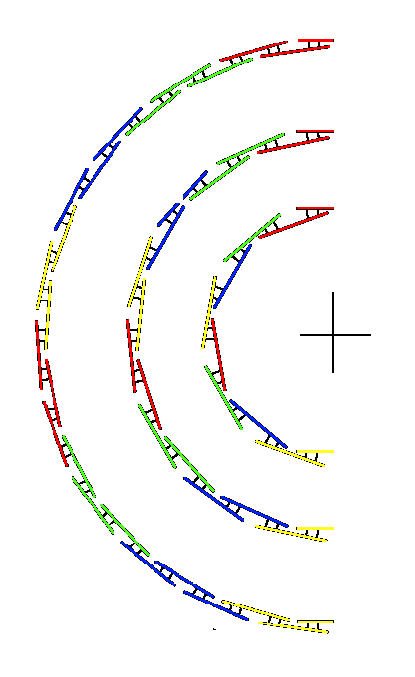
\epsfig{file = dcsPowerDistributionBPixA4603.eps, height = 56mm,
                         bbllx=18, bblly=24, bburx=175, bbury=316, clip=}}}
\put(34,0){\mbox{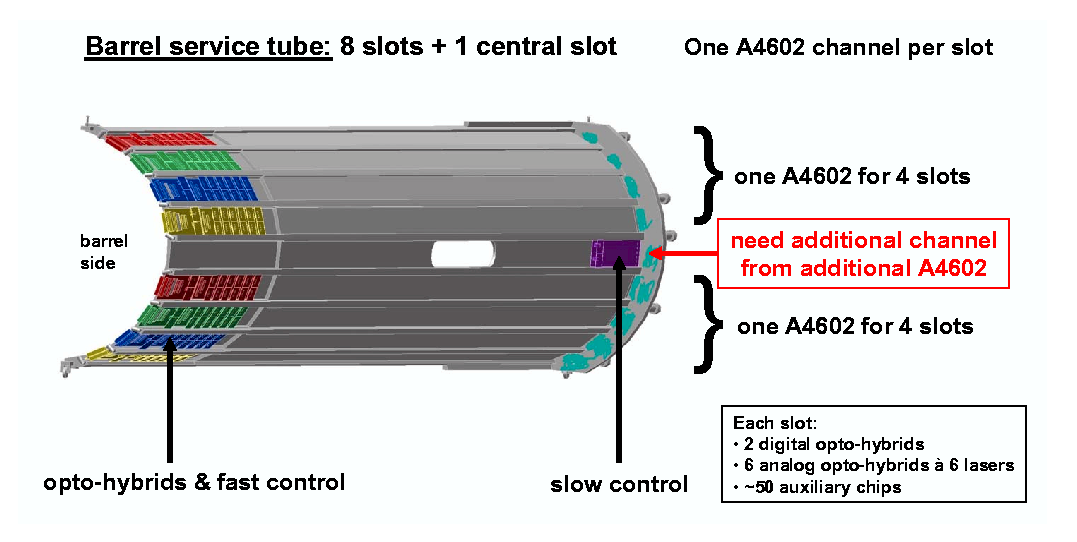
\epsfig{file = dcsPowerDistributionBPixA4602.eps, height = 62mm,
                         bbllx=25, bblly=21, bburx=502, bbury=252, clip=}}}
\end{picture}
    \caption{Distribution of power for detector operation and depletion of the sensors in the Barrel Pixel detector.
             The low voltages for operation of the ROCs and TBMs and the high voltages 
             for depletion of the pixel sensors are provided by boards of type A4603 (left). 
             One A4603 board provides high and low voltages for one sector of a shell (indicated by different colors).
             The first power supply unit provides power to the two inner layers,
             and the second power supply unit to the outer layer.
             The low voltages needed to operate the AOH, DOH and CCU mother boards are provided by boards of type A4602 (right).
             Per shell, a total of 9 channels is neccessary, 
             corresponding to two and a half A4602 type boards
             (the third board is shared between a pair of inner and outer shells at the same $z$ position).}
    \label{figure:dcsPowerDistributionBPix}
  \end{center}
\end{figure}

The DCS system consists of two major subsystems:
\begin{itemize}
\item The Siemens S7-300 Programable Logic Controller (PLC) system; and
\item The CAEN power supply and monitoring system.
\end{itemize}

As with the XDAQ-controlled devices, the system consists of control/monitoring
electronics elements and the on-detector components that it controls. 
In the DCS domain, two distinct sets of names are used 
to denote the control/monitoring electronics elements and the on-detector components they are connected to:
``hardware'' names denote the channels of the CAEN power supply system and of the Siemens S7-300 PLC system,
whereas the on-detector components (Read-out and Token Bit Manager chips, RTD temperature and HMX humidity sensors) are denoted ``logical'' names.
The association between the two sets of names is managed by cabling maps~\footnote{The cabling map information is currently handled by Excel spreadsheets; 
in the future, it is foreseen to store this information in database tables instead.}.

In this section we provide the naming conventions for the ``hardware'' names of the control/monitoring channels.
The ``logical'' names of the controlled/monitored devices are given in the section that
discusses the naming of on-detector components. 

The CAEN subsystem is built as distributed power supply system,
consisting of a SY1527 mainframe located in the US5 control room and two racks (X2F36 and X2F37) of power supply boards in the galley.
The purpose of distributing the power supply system between the control room and the galley
is to allow the mainframe to reside in an area of low radiation levels,
while bringing the power supply boards close to the detector
in order to reduce the voltage drop along the Multi-Service and Auxiliary Power cables.
In the Pixel detector control system, boards of type CAEN A4602 and A4603 are used.
The A4603 type boards provide high voltages for the depletion of the pixel sensors plus low voltages for the operation of the Read-out and Token Bit Manager chips.
The A4602 type boards provide low voltages for the operation of the Port Cards and CCU motherboards.
The A4602 and A4603 power supply boards are mounted in crates of type CAEN EASY 4000.
Each EASY 4000 crate can host up to 9 boards of either type, 
plus an interface card for interlock signals controlled by the Siemens S7-300 PLC system.
The A4602 and A4603 boards receive their power not from the mains,
but from Power Converters of type CAEN A3486 which convert the 220V AC mains to 48V DC.
The A3486 Power Converters are mounted in the same racks as the A4602 and A4603 boards.
The EASY 4000 crates as well as the A3486 Power Converters are controlled by means of CAEN A1676 branch controller cards,
plugged into slots of the SY1527 mainframe.

Each A4603 type board has two power supply units (PSU), numbered 0 and 1,
that each provide two low voltage channels, LV0 and LV1, and two high voltage channels, HV0 and HV1.
Of the two low voltage channels, 
LV0 provides a voltage of about 2.6 V for the Token Bit Manager chip and the digital (signal processing) part of the Read-out chip,
while LV1 provides a voltage of about 1.6 V for the analog (amplification and shaping of the charge signal) part of the Read-out chip.
Both high voltage channels, HV0 and HV1, can be independently set between 0-600V~\footnote{The
two independent high voltage channels allows for sensors that are closer to the beam axis
and hence receive a higher radiation dose to be operated at a higher bias voltage,
as described in section~\ref{sec:adp}.}.
Boards of the A4602 type provide four low voltage channels,
each delivering a voltage of about 2.5V 
for the operation of the electronic components present on the Port Cards and CCUM boards.

The names of the A4602 and A4603 boards are of the form~\footnote{The naming of the DCS control channels 
starts with a label representing either the Siemens or the CAEN subsystem, the so-called ``vendor node''.}:
\begin{displaymath}
\mbox{CAEN\_cmsPixelSY1527\_controller(00,01)\_crate(1-5)\_easyBoard(0-15).}
\end{displaymath}
The names for the high and low voltage channels provided by A4602 type boards and one PSU of A4603 type boards are of the form:
\begin{displaymath}
\mbox{CAEN\_cmsPixelSY1527\_controller(00,01)\_crate(1-5)\_easyBoard(0-15)\_channel(000-003).}
\end{displaymath}
The A3486 Power Converters are represented by names of the form:
\begin{displaymath}
\mbox{CAEN\_cmsPixelSY1527\_controller(00,01)\_crate(1-3)\_powerConverter}
\end{displaymath}
and their channels by:
\begin{displaymath}
\mbox{CAEN\_cmsPixelSY1527\_controller(00,01)\_crate(1-3)\_powerConverter\_channel(000, 001).}
\end{displaymath}
In each of the two racks X2F36 and X2F37, three Power Converters are installed.
Five out of the six channels power the high and low voltage channels of A4602 and A4603 boards
(one Power Converter channel is used per EASY 4000 crate).
The sixth Power Converter channel provides ``Service'' power for the electronics section of all boards in the rack.
%The rack layout of the CAEN power supply system is illustrated in figure~\ref{figure:CAENracks}.

The Siemens subsystem is located in rack S1G02 and consists of five crates
which are populated with modules of various types. 
The modules typically have several channels,
which are distinguished by a channel number. 

The names for the modules and channels are of the form\footnote{The numbering of the modules in the Siemens S7-300 PLC system starts at 4, not 0, 
in order to match the number assigned to the module in the Siemens Step7 PLC programming software.}:
\begin{displaymath}
\mbox{SIEMENS\_cms\_Pixel\_crate(1-5)\_module(4-11)}
\end{displaymath}
and 
\begin{displaymath}
\mbox{SIEMENS\_cms\_Pixel\_crate(1-5)\_module(4-11)\_channel(000-015),}
\end{displaymath}
respectively.

The types of modules used in the Siemens system for control and monitoring of the Pixel detector 
are ``RTD'' for Pt1000 temperature sensors, ``AI'' (analog input) for HMX humidity sensors,
``DI'' for digital inputs, ``DO'' for relay digital outputs,
``IM'' for ``Profi-Bus'' DP communication modules that connect the individual Siemens crates
and ``CPU'' for the Programmable Logic Controller (PLC)  which (pre)processes the temperature and humidity information 
and shuts-off (``interlocks'') the CAEN power supplies in case either the temperature or humidity values measured by the Siemens S7-300 PLC system
constitute a risk for the safe operation of the Pixel detector.
The CPU module also contains an Ethernet interface which connects the PLC system to rack-mounted Windows PCs
running the ``Prozess Visualisierungs und Steuerungs Software'' (PVSS).


\section{Association of Control Channels and On-Detector Devices}

In order to be able to configure, control and monitor the physical devices
on the detector, we have to send commands and data to registers of individual 
chips. This requires us to associate a VME-control channel with the
on-detector device that it controls.
This association is complex because it has two parts:
\begin{itemize}
\item Association with a VME control channel; and
\item Association with either an I$^{2}$C or PSI$^{2}$C address.
\end{itemize}

This association is made by looking up the relevant information, derived from
the names, in a small database table.

%Few concerns \& claims:
% \textcolor{red}{This section needs to be expanded with some examples}


\subsection{Association of a Device to its VME Control Channel}

There are three basic types of VME control modules, leading to three basic
types of association:
\begin{enumerate}
\item A channel of a PxlFEC controls all the devices (ROCs and TBMs) on each 
of the 6 panels attached to one Port Card. (The Port Card actually connects 
to the TBMs through the Gate Keeper chip on the Port Card and then through the 
Adapter Board to the panel on which the TBM actually resides. 
Since the Adapter Board and the Gate Keeper chip are not programmable and there is
a direct correspondence between a Port Card and them, we reduce the 
complexity by pretending that the Port Card connects directly to all the 
Panels and corresponding TBMs that it controls);
\item One channel of the TrkFEC connects to one CCUM board,
      which connects to the DCU chips on the 8 Port Cards; and
\item Each of the 36 inputs of a PxlFED receives data from one 
panel (actually its TBM).  
\end{enumerate}

For illustration, a schematic block diagram of the connections between the PxlFEC, TrkFEC and FED VME modules,
the CCUM boards and Port Cards and TBMs and ROCs is shown in figure~\ref{figure:cabling}
(the Port Cards, TBMs and ROCs are represented by ``quadrants'' in the figure).


\subsubsection{PxlFEC}

To actually determine which PxlFEC channel controls the operation of a 
specific readout chip or a particular pixel, we can use the geometry of
the detector. Since the name contains the whole address including the  panel 
number, the Port Card is determined by:
\begin{equation}
{\rm Port \ Card \ number} \ = {\rm Int} \, 
[({\rm Blade \  number} \ - \ 1 )/3] \ + \ 1
\end{equation}
The association of the Port Card to a PxlFEC channel can be looked up in a 
small database table.

An example of such an association is:
\begin{displaymath}
\mbox{S1G01e\_S06-PxlFEC\_Ch1}\ \rightarrow\ \mbox{FPix\_BpO\_D1\_PRT1(PRT2),}
\end{displaymath}


\subsubsection{TrkFEC}

To actually determine which TrkFEC channel controls the operation of a 
chip on a Port Card such as a PLL, we can again use the geometry to
the detector. Since the name contains the whole address down to the  Port 
Card number, the CCUM is determined by: 
\begin{equation}
{\rm CCUM} \ = {\rm Int} [ ({\rm Port \ Card \ number} \ - \ 1 )/ 4] \ + \ 1
\end{equation}
The association of the CCUM to the TrkFEC can be looked up in a small
database table again.

An example of such an association is:
\begin{displaymath}
\mbox{S1G01e\_S17-TrkFEC\_Ch3}\ \rightarrow\ \mbox{FPix\_BpO\_CCUM,}\ 
\mbox{FPix\_BpO\_CCUM\_CCU1}\ \rightarrow\ \mbox{FPix\_BpO\_D1\_PRT1(PRT2).}
\end{displaymath}


\subsubsection{FED}

To determine which FED channel is connected to which readout chip (or pixel), one 
needs to deduce the Port Card number from the panel number. This is determined
by the formula given above for the PxlFEC. Another small database table
then associates the Port Card to the FED channel.

An example of such an association is:
\begin{displaymath}
\mbox{S1G03e\_S10-PxlFED\_Ch1}\ \rightarrow\ \mbox{FPix\_BpO\_D1\_PRT1(PRT2).}
\end{displaymath}


\subsubsection{Cable Connection Databases}

At the beginning of the experiment, it is likely that the FED and FEC channels
will be ordered in a consecutive manner so that it would be possible to 
make a simple numerical association between the channel number and the readout chip 
once the Port Card or CCUM number is determined. 
We have no objection to this. 
If it is put into the code, there needs to be a method of changing the numerical
association if it becomes necessary to move a cable to a different input in
the event of a failure of a channel or group of channels in one of these 
modules. For this reason, we prefer to use small database tables. 
However, these kinds of issues are left to the person doing the actual implementation.

In total, four PxlFEDs are used to read out all readout chips on the +z side of the FPix detector;
only one PxlFEC is needed to configure these ROCs;
and two channels of the TrkFEC are used control the two CCUMs (one per half-cylinder), 
that serve as I$^{2}$C masters to control the standard I$^{2}$2C networks to the Port Cards. 


%\begin{figure}[hbtp]   
%  \begin{center}   
%        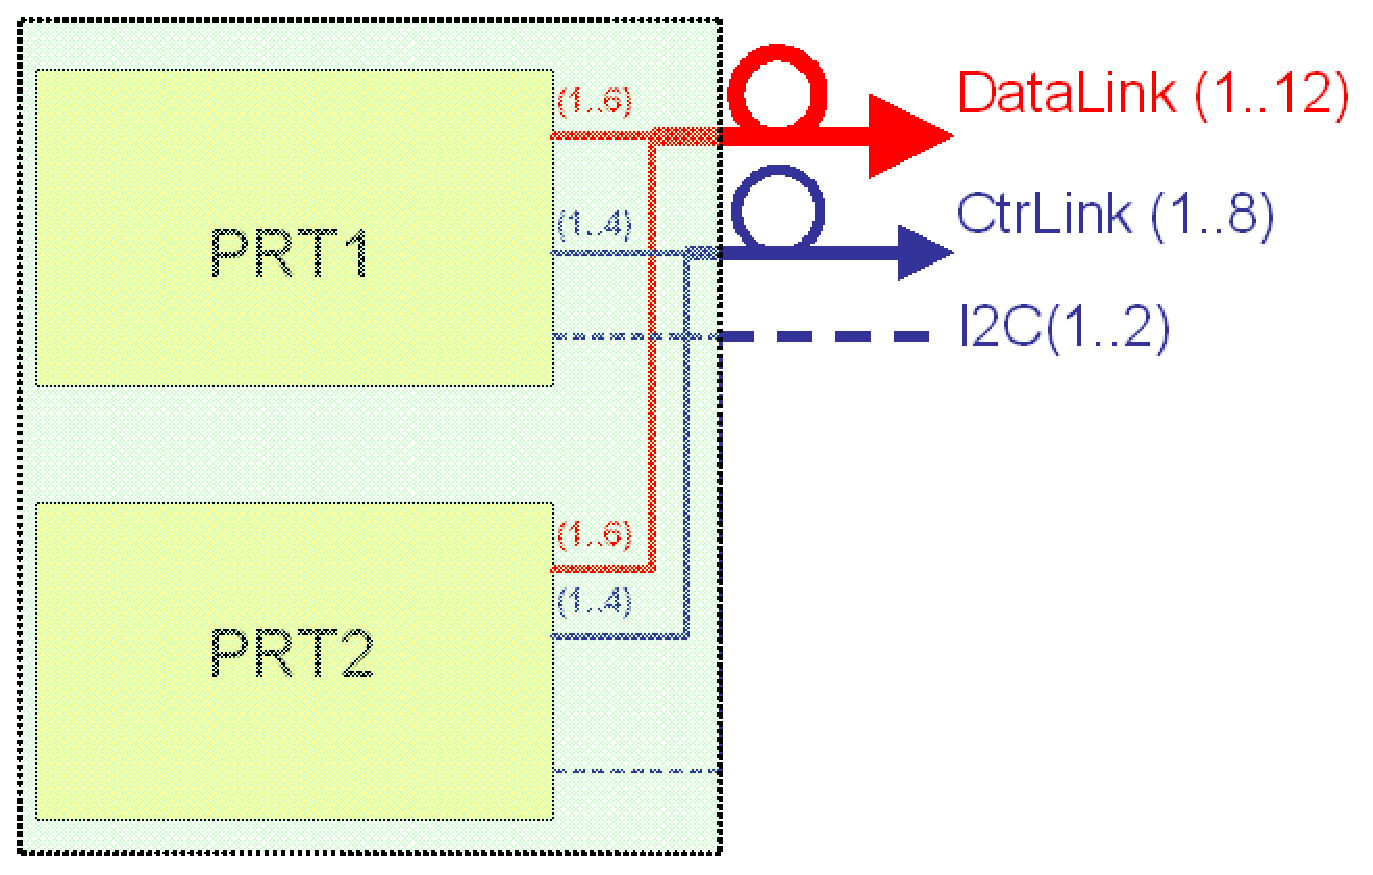
\includegraphics[width =0.5\textwidth]{qua.eps}   
%    \caption{A logical organization of Port Cards. See the content 
%for detailed descriptions. }   
%    \label{figure:qua}   
%  \end{center}   
%\end{figure} 
 
%For the last example, the connection from the CCU to Port Cards contains two 
%I$^{2}$2C networks. (???)


\begin{figure}[hbtp]   
  \begin{center}   
        \includegraphics[width =0.9\textwidth]{cabling.eps}   
    \caption{A block diagram of the positive z-axis side of the Forward Pixel detector. 
             The connections are identified between the VME modules and quadrants. 
             Here red lines denote 12-channel optical fibers; 
             blue lines also denote 12-channel optical fibers, however, 
             only eight of these 12 channels are used.
             Each black line between a quadrant and a CCU denotes two I$^{2}$C networks.
             The first I$^{2}$C network connects to CCUs 1 and 3 and the second to CCUs 2 and 4.}
    \label{figure:cabling} 
  \end{center}   
\end{figure} 


%Few concerns:
%\begin{itemize}
%\item \textcolor{red}{At this stage, the numbering  within a CtrLink or 
%DataLink is
%not possible to identify. However, it is proposed that the 
%optical links from the Port Card of smaller index occupy the 
%low six (one to six) or four (one to four) channels of the 
%optical connector; the 
%optical links from the Port Card of larger index occupy the high 
%six (six to twelve) or four (eight to twelve) channels of the 
%optical connector }
%\item \textcolor{red}{As a summary, this proposes of one TrkFEC, 
%two PxlFEC, and 
%eight PxlFED to operate and control the Forward Pixel detector. }
%\end{itemize}


\subsection{Association of a Device with its I$^{2}$C Address}

One VME channel controls many hardware devices by means of
commands issued over an I$^{2}$C network. To complete the control path, we have to 
know the following:
\begin{itemize}
\item for devices controlled by the TrkFEC, the CCUM and the Bus Controller
Number (1-8); and
\item for devices controlled by the PxlFEC, the Port Card and Hub and 
Port Address.
\end{itemize}

An example of the steps required to use the name to determine a very
common association is shown in fig.~\ref{figure:associations}.

\subsection{Association of Data to an On-Detector Devices}

Elements of the detector may have programmable settings, such as thresholds,
voltages, mask bits, or operating modes, to name some of the more common ones.
Each readable or writable register of each device has a name. The name is an 
extension of the parent detector element with the register name appended.
These names appear in database tables along with the data that is either to be 
used in settings or corresponds to recorded readings. Thus the name is used
as an database index or key to 
associate a register with data; to determine, using a 
combination of operations on the name and database lookups, the controlling VME
channel; and to retrieve the relevant I$^{2}$C or PSI$^{2}$C addresses
from the name and VME channel number by means of database look-ups;
in order to complete the control path.


\begin{figure}
\begin{center}   
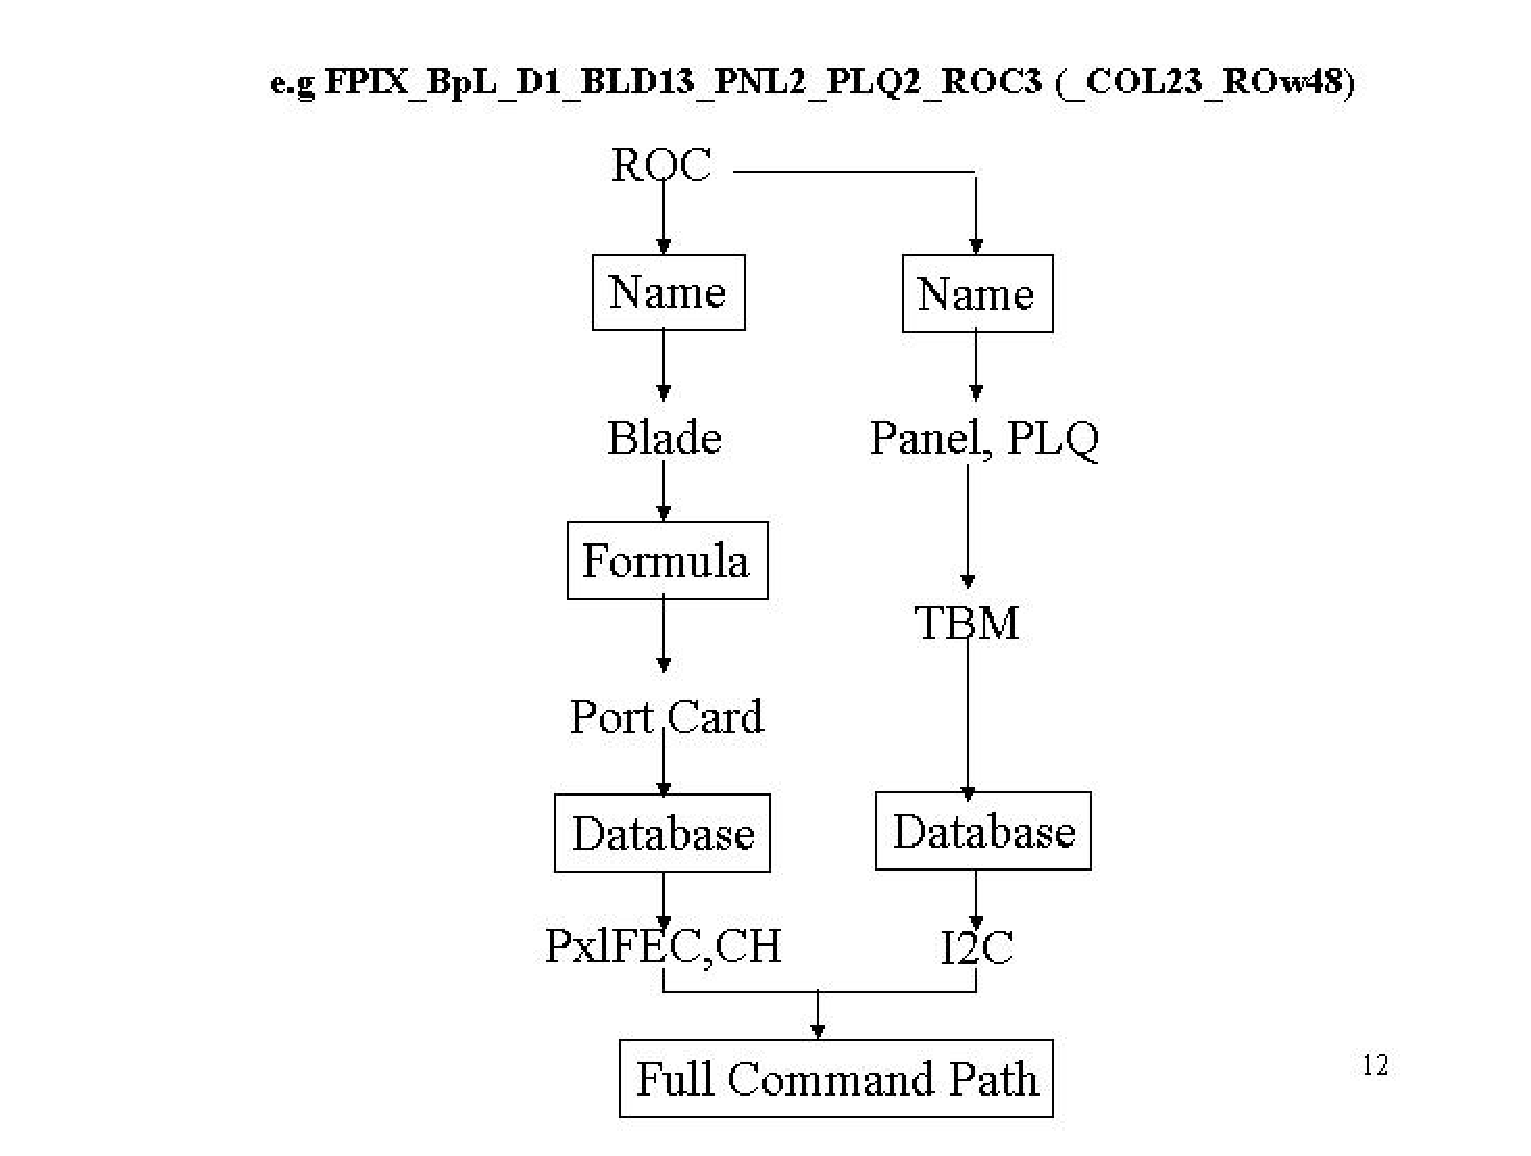
\includegraphics[width =0.9\textwidth]{association_eg.eps}   
\caption{Illustration of the interplay of the naming convention, various
geometric rules, and the database in establishing a complete control
path and the data for an on-detector component.     
\label{figure:associations} }
\end{center}
\end{figure}


%  reference
%%%%%%%%%%%%%%%%%%%%%%%%%%%%%%%%%%%%%%%%%%%%%%%%%%%%%%%%%%%%%%%%%
\begin{thebibliography}{9}

\bibitem{integration} Integration of Run Control and Detector Control Systems,
CMS Internal Note IN 2005/015, CMS Trigger/DAQ Group, J. Varela, Editor

\bibitem{DataModel} N. Amapane {\it et al.}, Models of Data for Tracking 
Detectors, CMS internal note 2005/xxx.

\bibitem{roc_reg} U. Langenegger, A. Starodumov, P. Trub, Test and 
Qualification Procedures of the CMS Pixel Barrel Modules, CMS Internal
Note 2006/006.

  \bibitem{LLD} G. Cervelli {\it et al.}, Radiation Tolerant Linear Laser 
Driver IC (reference and technical manual), CERN-EP Division, Geneva, 
Switzerland, 2003.
  
  \bibitem{DCU} G. Magazzu, A. Marchioro, and P. Moreira, DCUF User Guide, 
CERN-EP/MIC, Geneva, Switzerland, 2003.


  \bibitem{TPLL} P. Placidi, A. Marchioro, and P. Moreira, CMS Trakcer PLL 
Reference Manual, CERN-EP/MIC, Geneva, Switzerland, 2000.

  \bibitem{DELAY25} H. Correia {\it et al.}, Delay25, CERN-EP/MIC, Geneva, 
Switzerland, 2004.

\bibitem{CCU} A. Marchioro, C. Ljuslin, and C. Paillard, CCU25 - Communication and Control Unit ASIC for Embedded Slow Control (draft). 
\end{thebibliography}
 


\pagebreak
\begin{appendix}

Eventually, this appendix will contain the names of every register 
for every chip in the system. These names are usually defined in the chip
specification documents.

\section{Forward PIxel Panel readout and Control Sequence Issues}

One complication with respect to the Forward Pixel System, is that the
two types of panels, one with 3 plaquettes and one with 4 plaquettes, each come
in two varieties. The distinction is whether the TBM is mounted on a tab
to left of the vertical centerline, a so-called ``left-handed'' panel, or to 
the right of the centerline, a so-called ``right-handed'' panel. The four types
of panel are then referred to as 3L, 4L, 3R, and 4R. 

From a geometric point of view, this is only significant for the panels
on the four blades of each half-ring that are nearest the vertical symmetry
plane, that is the blades numbered 1 and 12. For these, the panelsmust be 
chosen so that the TBM tabs are away from the plane (otherwise it would be hard
to position the two half-cylinders so as to minimize the gap between them. For
all other blades, the choice of whether to use left-handed or right-handed
panels is arbitrary and, in fact, is made at the time of half-ring assembly
based on  what fully-tested and approved panels happen to be available.

This arbitrariness becomes a problem because the order in which the ROCs
are readout is different from the  left-handed and right-handed
panels. The data from the ROCs appear as a stream of information to the 
Front-End Driver (FED) boards. The data stream does not contain a ROC-id.
The ROC-id depends on the order in which the ROC appears in the data stream.
There is at least a header for eavery ROC even if the ROC contained no
data. Since the order of the readout of the ROCs is different for the
lef-handed and right-handed panels and the choice of which to use is
arbitrary, database tables are needed to make all the necessary associations.
\begin{itemize}
\item There has to be a table that
specifies which type of panel, L or R, is used in each location, defined
by its ``RLI.''  This can only be provided once each half-ring is assembled 
and installed in its service cylinder.
\item There has to be a table that describes for each of the four panel types,
the number of the ROC and the order that it will appear in the data stream
to the FED. In addition, in order to control the ROC, it needs control 
path designation, which takes the form of a ``port number'' and ``PSI$^2$C''
address. These associations are determined by the hardware and given in
tables~\ref{table:plaq_fed_4R}, \ref{table:plaq_fed_3R}, 
\ref{table:plaq_fed_4L}, and \ref{table:plaq_fed_3L}.
\end{itemize} 


\begin{table}[htb]
    \caption{
Association for panel type 4R of plaquette and ROC to order
(1-21)  in the event stream, referred to as ultrablack number, port number, 
and PSI$^{2}$C address. These assignments all refer to a single panel, read 
out by a single TBM. ``hub'' refers to TBM Hub.
}
    \label{table:plaq_fed_4R}
    \begin{center}
      \begin{tabular}{l|l|cccc} \hline
Panel & Plaq & Port & ROC & ROC & ROC \\
Type  & Number & Number & Number & I$^2$C Addr & Number \\
      &        &        & on Plaq &            & in FED \\ \hline
4R & 1 & 2 &  0 & 1 & 21 \\
   &   &   &  1 & 0 & 20 \\
   & 2 & 3 &  0 & 3 & 17 \\
   &   &   &  1 & 4 & 18 \\
   &   &   &  2 & 5 & 19 \\
   &   &   &  3 & 0 & 14 \\
   &   &   &  4 & 1 & 15 \\
   &   &   &  5 & 2 & 16 \\
   & 3 & 1 &  0 & 4 & 10 \\
   &   &   &  1 & 5 & 11 \\
   &   &   &  2 & 6 & 12 \\
   &   &   &  3 & 7 & 13 \\
   &   &   &  4 & 0 &  6 \\
   &   &   &  5 & 1 &  7 \\
   &   &   &  6 & 2 &  8 \\
   &   &   &  7 & 3 &  9 \\
   & 4 & 0 &  0 & 4 &  5 \\
   &   &   &  1 & 3 &  4 \\
   &   &   &  2 & 2 &  3 \\
   &   &   &  3 & 1 &  2 \\
   &   &   &  4 & 0 &  1 \\
      \end{tabular}
    \end{center}
  \end{table}


\begin{table}[htb]
    \caption{
Association for panel type 3R of plaquette and ROC to order
(1-24)  in the event stream, referred to as ultrablack number, port number, 
and PSI$^{2}$C address. These assignments all refer to a single panel, read 
out by a single TBM. ``hub'' refers to TBM Hub.
}
    \label{table:plaq_fed_3R}
    \begin{center}
      \begin{tabular}{l|l|cccc} \hline
Panel & Plaq & Port & ROC & ROC & ROC \\
Type  & Number & Number & Number & I$^2$C Addr & Number \\
      &        &        & on Plaq &            & in FED \\ \hline
3R & 1 & 2 &  0 & 0 & 22 \\
   &   &   &  1 & 1 & 23 \\
   &   &   &  2 & 2 & 24 \\
   &   &   &  3 & 3 & 19 \\
   &   &   &  4 & 4 & 20 \\
   &   &   &  5 & 5 & 21 \\
   & 2 & 1 &  0 & 0 & 15 \\
   &   &   &  1 & 1 & 16 \\
   &   &   &  2 & 2 & 17 \\
   &   &   &  3 & 3 & 18 \\
   &   &   &  4 & 4 & 11 \\
   &   &   &  5 & 5 & 12 \\
   &   &   &  6 & 6 & 13 \\
   &   &   &  7 & 7 & 14 \\
   & 3 & 0 &  0 & 0 &  6 \\
   &   &   &  1 & 1 &  7 \\
   &   &   &  2 & 2 &  8 \\
   &   &   &  3 & 3 &  9 \\
   &   &   &  4 & 4 & 10 \\
   &   &   &  5 & 5 &  1 \\
   &   &   &  6 & 6 &  2 \\
   &   &   &  7 & 7 &  3 \\
   &   &   &  8 & 8 &  4 \\
   &   &   &  9 & 9 &  5 \\
      \end{tabular}
    \end{center}
  \end{table}


\begin{table}[htb]
    \caption{
Association for panel type 4L of plaquette and ROC to order
(1-21)  in the event stream, referred to as ultrablack number, port number, 
and PSI$^{2}$C address. These assignments all refer to a single panel, read 
out by a single TBM. ``hub'' refers to TBM Hub.
}
    \label{table:plaq_fed_4L}
    \begin{center}
      \begin{tabular}{l|l|cccc} \hline
Panel & Plaq & Port & ROC & ROC & ROC \\
Type  & Number & Number & Number & I$^2$C Addr & Number \\
      &        &        & on Plaq &            & in FED \\ \hline
4L & 1 & 1 &  0 & 1 &  2 \\
   & 1 & 1 &  1 & 0 &  1 \\
   & 2 & 0 &  0 & 0 &  3 \\
   & 2 & 0 &  1 & 1 &  4 \\
   & 2 & 0  & 2 & 2 &  5 \\
   & 2 & 0  & 3 & 3 &  6 \\
   & 2 & 0  & 4 & 4 &  7 \\
   & 2 & 0  & 5 & 5 &  8 \\
   & 3 & 2 &  0 & 0 &  9 \\
   & 3 & 2 &  1 & 1 & 10 \\
   & 3 & 2 &  2 & 2 & 11 \\
   & 3 & 2 &  3 & 3 & 12 \\
   & 3 & 2 &  4 & 4 & 13 \\
   & 3 & 2 &  5 & 5 & 14 \\
   & 3 & 2 &  6 & 6 & 15 \\
   & 3 & 2 &  7 & 7 & 16 \\
   & 4 & 3 &  0 & 4 &  21 \\
   &   &   &  1 & 3 &  20 \\
   &   &   &  2 & 2 &  19 \\
   &   &   &  3 & 1 &  18 \\
   &   &   &  4 & 0 &  17 \\
      \end{tabular}
    \end{center}
  \end{table}


\begin{table}[htb]
    \caption{
Association for panel type 3L of plaquette and ROC to order
(1-24)  in the event stream, referred to as ultrablack number, port number, 
and PSI$^{2}$C address. These assignments all refer to a single panel, read 
out by a single TBM. ``hub'' refers to TBM Hub.
}
    \label{table:plaq_fed_3L}
    \begin{center}
      \begin{tabular}{l|l|cccc} \hline
Panel & Plaq & Port & ROC & ROC & ROC \\
Type  & Number & Number & Number & I$^2$C Addr & Number \\
      &        &        & on Plaq &            & in FED \\ \hline
3L & 1 & 1 &  0 & 0 &  1 \\
   &   &   &  1 & 1 &  2 \\
   &   &   &  2 & 2 &  3 \\
   &   &   &  3 & 3 &  4 \\
   &   &   &  4 & 4 &  5 \\
   &   &   &  5 & 5 &  6 \\
   & 2 & 2 &  0 & 0 &  7 \\
   &   &   &  1 & 1 &  8 \\
   &   &   &  2 & 2 &  9 \\
   &   &   &  3 & 3 & 10 \\
   &   &   &  4 & 4 & 11 \\
   &   &   &  5 & 5 & 12 \\
   &   &   &  6 & 6 & 13 \\
   &   &   &  7 & 7 & 14 \\
   & 3 & 3 &  0 & 0 & 15 \\
   &   &   &  1 & 1 & 16 \\
   &   &   &  2 & 2 & 17 \\
   &   &   &  3 & 3 & 18 \\
   &   &   &  4 & 4 & 19 \\
   &   &   &  5 & 5 & 20 \\
   &   &   &  6 & 6 & 21 \\
   &   &   &  7 & 7 & 22 \\
   &   &   &  8 & 8 & 23 \\
   &   &   &  9 & 9 & 24 \\
      \end{tabular}
    \end{center}
  \end{table}


\section{Readout Chip}

The names of the registers of the pixel readout chips are taken from~\cite{roc_reg}.

\begin{description}
\item[Vdig] Digital Voltage Regulator
\item[Vana] Analog Voltage Regulator
\item[Vsf] Sample-and-Hold Buffer Power Regulator
\item[Vcomp]
\item[Vleak\_comp] Sensor Leakage Current Compensation
\item[VrgPr] Preamplifier Feedback
\item[VwllPr] Preamplifier Feedback
\item[VrgSh] Shaper Feedback
\item[VwllSh] Shaper Feedback
\item[VHldDel] Hold Delay
\item[Vtrim] Pixel trimming Voltage
\item[Vthr\_comp] Comparator Threshold
\item[VIBias\_bus]  
\item[Vbias\_sf] Source Follower
\item[VOffsetOp] Positive offset for analog Pulse-Height Amplification 
\item[VIbiasOp] 
\item[VOffsetRO] Negative offset for analog Pulse-Height Amplification 
\item[VIon]
\item[VIbias\_PH] Amplification of analog Pulse-Height
\item[Ibias\_DAC] Amplification of digital Levels (ROC Ultra-Black, Black and Address Levels) 
\item[VIbias\_roc] Output Amplifier
\item[VIColOr] 
\item[Vnpix]
\item[VSumCol]
\item[Vcal] Calibration Signal Voltage Regulator
\item[CalDel] Delay between Calibration Signal and actual Charge Injection into either the Calibration Capacitor or the Sensor
\item[RangeTemp] Control Register for readout of Temperature Sensor
\item[CtrlReg] Chip Control Register
\item[WBC] Trigger Latency
\end{description}


\section{TBM \label{app:tbm}}

The TBM has some configuration registers. 
%The names given are made up by me.
%I do not really know much about the TBM registers. They should be 
%specified and named by the chip designer, Ed Bartz.

\begin{description}
\item[TBM\_ana1] Analog adjustment 1
\item[TBM\_ana2] Analog adjustment 2
\item[TBM\_ana3] Analog adjustment 3
\item[TBM\_mode] Single vs. Dual TBM mode
\item[TBM\_speed] Readout speed
\item[TBM\_csr]Trigger injection
\item[Stk\_rd] Stack Readback
\item[Chp\_disable] chip disabling (bypassing?)
\end{description}

\section{Linear Laser Driver \label{app:lld}}

The Linear Laser Driver (LLD) used in the Pixel detector is 
described in~\cite{LLD}. Here we just summarize the relevant 
information about its I$^2$C interface.

The I$^2$C interface of the LLD is a standard I$^2$C protocol. 
Using a 7-bit addressing mode, the 
highest five bits are decoded as the chip address, which are set 
by connecting to external pull-down resistors when power up. 
This also means that there are at most 32 LLDs in any I$^2$C network.  
The lowest two bits are used to access the four internal registers:
REG0 (0x0), REG1 (0x1), REG2 (0x2), and GAINREG (0x3). These registers 
are seven bits wide. REG0, REG1, and REG2 are used to adjust the 
bias current for channels 0, 1 and 2, respectively. 
For the DOH, initially these 
registers are set to 0x70. The GAINREG register sets the gain for 
each channel, with two bits per channel. 
The highest bit is used to flag 
the Single Event Upset (SEU). For DOHs, the initial gain is set to 
maximum (0x2) for each channel. 

For pixel DOHs, there is only one LLD used. A convenient way to identify 
registers within DOH (only registers belong to LLD) could be:
\begin{description}
\item[REG0]
\item[REG1]
\item[REG2]
\item[GAINREG]
\end{description}
However, for a pixel AOH, two LLDs are used. 
We propose names similar to those of DOHs:
\begin{description}
\item[REG0]
\item[REG1]
\item[REG2]
\item[GAINREG0]
\item[REG3]
\item[REG4]
\item[REG5]
\item[GAINREG1]
\end{description}


\section{Analog Level Shifter \label{app:alt}}


\section{Detector Control Unit \label{app:dcu}}

The Detector Control Unit (DCU) is described in~\cite{DCU}. 
Here we only summarize the I$^2$C interface. 
The DCU I$^2$C interface is based on the standard I$^2$C protocol. In a 
7-bit addressing mode, the most significant four bits are compared 
with the chip address. The lowest three bits are then used to 
address the eight internal registers: 
\begin{description}
\item[CREG]
\item[SHREG]
\item[AREG]
\item[LREG]
\item[TREG]
\item[IDLREG]
\item[IDMREG]
\item[IDHREG]
\end{description}
which correspond to the addresses 0x0 to 0x7, respectively. 

%
% CV: This has most probably been changed in the meantime -> ask Sergey Los !!
%
%There are eight input channels for each DCU chip. Since the last channel (0x7) 
%is used to connect the embedded temperature sensor, there
%are at most seven external inputs. 



\section{Tracker PLL}

The Tracker PLL~\cite{TPLL} (TPLL) also has a standard I2C interface. It uses a 7-bit 
addressing mode. The five most significant bits are compared to 
identify the chip address. The lowest two bits are then used to 
identify the five internal registers: CTR1 (0x0), CTR2 (0x1), CTR3 (0x2), CTR4 
(0x3) and CTR5 (0x3). 
\begin{description}
\item[CTR1]
\item[CTR2]
\item[CTR3]
\item[CTR4]
\item[CTR5] ,
\end{description}
corresponding to the addresses 0x0 to 0x3. 
Note that CTR4 and CTR5 share the same I2C address, and 
they are distinguished by the bit five of CTR2.

\section{Delay 25 \label{app:del}}

The I$^2$C interface of the Delay 25 chip~\cite{DELAY25} is based on 
a standard I$^2$C protocol. Using a 7-bit addressing mode, the most significant four 
bits are used to decode the chip address, and the
lowest three bits are used to access the six control registers: 
\begin{description}
\item[CR0]
\item[CR1]
\item[CR2]
\item[CR3]
\item[CR4]
\item[GCR] ,
\end{description}
which correspond to the addresses 0x0 to 0x5, respectively. 


\section{CCU}

The CCU chip has a quite complex internal structure, a detailed description 
of which can be found in~\cite{CCU}. 
The following list gives an overview over the registers of the CCU node controller,
including its control and status registers:
\begin{description}
\item[CRA]
\item[CRB]
\item[CRC]
\item[CRD]
\item[CRE]
\item[SRA]
\item[SRB]
\item[SRC]
\item[SRD]
\item[SRE]
\item[SRF] .
\end{description}
The allocation of channels can be summarized as follows:
\begin{description}
\item[NC] channel0, the node controller
\item[I2C1-I2C16] I$^2$C channels from 1 to 16. 
\item[PIO1-PIO4] PIO channels from 1 to 4 
\item[MEM] Memory channel
\item[TRG] Trigger distribution channel
\item[IR0-IR1] Interrupt channels.
\end{description}

In each CCU chip, there are other registers in addition, 
of which only an incomplete list is presented here:
\begin{description}
\item[MSK] Mask register for logical operation
\item[WIN1L, WIN1H, WIN2L, WIN2H] Memory bus window registers 
\item[GCR, SR, DDRA, DREG] Parallel I/O bus registers.
\end{description}


\section{Cross reference of various pixel indices}
\label{app:CrossReferencePixelIndices}

The plaquettes and modules use ROC addresses called ``ROC Location Indices,'' or RLIs.
There are several other address schemes  that apply to ROCs at various levels of hardware and
software. These are cross-referenced in the tables below.


\end{appendix}
\end{document}


